\documentclass[twoside,11pt,nocover,
  printed, %% This option enables the default options for the
           %% digital version of a document. Replace with `printed`
           %% to enable the default options for the printed version
           %% of a document.
  notable,   %% Causes the coloring of tables. Replace with `notable`
           %% to restore plain tables.
  nolof,     %% Prints the List of Figures. Replace with `nolof` to
           %% hide the List of Figures.
  nolot,     %% Prints the List of Tables. Replace with `nolot` to
           %% hide the List of Tables.
  nopalatino, %% Disable palatino globally, enable later using packages
              %% for normal text, not mathmode
  %% More options are listed in the user guide at
  %% <http://mirrors.ctan.org/macros/latex/contrib/fithesis/guide/mu/fi.pdf>.
]{fithesis3}

%% The following section sets up the locales used in the thesis.
\usepackage[resetfonts]{cmap} %% cmap makes the PDF searchable and copyable

% Following packages are enabled by fithesis palatino option
\usepackage{lmodern}
% \usepackage{mathpazo} % Palatino font for mathematics, breaks nice \mathbb
\usepackage{tgpagella} % Palatino font for normal text

\usepackage[T1]{fontenc}
\usepackage[
  main=english, %% By using `czech` or `slovak` as the main locale
                %% instead of `english`, you can typeset the thesis
                %% in either Czech or Slovak, respectively.
  czech,british %% The additional keys allow
]{babel}        %% foreign texts to be typeset as follows:
%%
%%   \begin{otherlanguage}{czech}   ... \end{otherlanguage}

%% The following section sets up the metadata of the thesis.
\thesissetup{
    date          = \the\year/\the\month/\the\day,
    university    = mu,
    faculty       = fi,
    type          = d,
    author        = Petr Velan,
    gender        = m,
    advisor       = {doc. Ing. Pavel Čeleda, Ph.D.},
    title         = {Application-Aware Flow Monitoring},
    TeXtitle      = {Application-Aware Flow Monitoring},
    keywords      = {network, monitoring, measurement, flow, application flow, NetFlow, IPFIX, encryption, performance, 100Gbps},
    TeXkeywords   = {network, monitoring, measurement, flow, application flow, NetFlow, IPFIX, encryption, performance, 100\,Gbps},
    bib           = {bibliography.bib,publications.bib,rfcused.bib},
}
\thesislong{abstract}{%

\noindent The Internet has become a crucial medium for business, entertainment, communication, learning, access to information, and other human endeavours. As the society becomes increasingly dependent upon the availability and security of online services, the revenue from disrupting the normal operation of these services increases as well. Gaining unauthorised access, disrupting functionality, stealing and selling confidential data, and impersonation are only a few examples of these disruptions. Various systems, such as firewalls and anti-virus software, are intended to thwart these attacks and reduce the associated risks. To protect users on their networks, administrators often deploy network monitoring systems to detect and mitigate the threats.

Network flow monitoring is an instrument which allows observing traffic passing through given point in the network and gathering aggregated information about the observed network connections. The aggregated nature of provided information allows to scale the flow monitoring to high-speed networks and monitor traffic rates up to and including hundreds of gigabits per second. Flow data is mainly used for security purposes. However, due to its versatility, it is often used for network management tasks, such as capacity planning and accounting, as well. As both network communication protocols and attack vectors are becoming increasingly sophisticated, the flow monitoring needs to evolve as well. The current trends for flow monitoring are the extraction of supplementary information from application protocols, identification of encrypted traffic, and monitoring of high-speed networks.

% generic contribution summary
This thesis contributes to the progression of flow monitoring by exploring the possibilities unlocked by extending the flow data with application-specific information. We show how the construction of flows is affected by the addition, present the benefits to traffic analysis and assess the inevitable performance loss. To compensate for the lost performance several novel optimisation techniques are proposed for the flow monitoring process. Recognizing that the increasing deployment of encryption is going to limit the benefits of application flow monitoring, we perform a survey of methods for measurement of encrypted traffic. The thesis is concluded by an outlook towards future possibilities for flow monitoring advancement.

% specific contributions
The first contribution of this thesis is a revised definition of flow that attempts to improve and update currently used definitions so that it better matches current flow monitoring practices. A formal definition of flow, together with algorithms for flow construction based on this definition is provided as well. We demonstrate that the revised flow definition allows for use cases that were not covered by NetFlow v9 and IPFIX definitions, such as monitoring of traffic containing fragmented packets.

Using the revised terminology and definitions, we focus on application flow monitoring, which is one of the current trends in flow monitoring. Firstly, an overview of the state of application flow monitoring is provided. Secondly, practical definitions of application flow and application flow record are given to circumscribe application flow monitoring. Thirdly, an experimental study on the design of an HTTP application protocol parser is presented. The study quantifies how application flow monitoring increases the demand for computational resources and decreases the performance of the flow monitoring system.

The application flow monitoring provides new data for traffic analysis. We study several use cases for which the application flow monitoring can be applied in detail. The first one uses information from HTTP headers to detect new classes of attacks on the application layer. The second one shows how the additional information can be used to analyse utilisation of IPv6 transition mechanisms. Then, we show that adding geolocation information to flow records can be used for advanced traffic analysis. And last, a method for characterising network traffic is described. It allows comparing multiple network traces and searching for similarities.

The monitoring of high-speed networks is one of the current trends in flow monitoring. Firstly, we describe the state-of-the-art in this area. Secondly, we identify and propose multiple optimisations including those that rely on programmable network interface cards. Some of these optimisations are then used to build and demonstrate a high-density flow monitoring system capable of processing sixteen 10\,Gb links in a single box.

Classification of encrypted traffic and identification of applications using encryption has become a widely researched topic in the last decade. A survey of methods for measurement of encrypted traffic is, therefore, one of the contributions of this thesis. We show that surprisingly detailed information can be obtained using these methods. In specific cases, even the content of the encrypted connection can be established.

This work concludes with a vision for the future of the flow monitoring. We identify several directions of future research of flow monitoring and a novel approach to monitoring of tunnelled traffic and application layer is proposed. We believe that the perception of the whole application flow monitoring should be revised to facilitate future demands for more complete and better-structured data.
}

\thesislong{thanks}{
I would like to thank my advisor, colleagues, and fellow researchers for their input and insights that helped to shape my research and this thesis. Furthermore, I could have hardly finished this work without the relentless support of my friends and family. They have my eternal gratitude.
}

\usepackage{makeidx}      %% The `makeidx` package contains
\makeindex                %% helper commands for index typesetting.
%% These additional packages are used within the document:
% \usepackage{paralist}     %% Compact list environments
\usepackage{amsmath}      %% Mathematics
\usepackage{amsthm}
\usepackage{amsfonts}
\usepackage[hyphens]{url} %% Hyperlinks
% \usepackage{markdown}     %% Lightweight Markup

% override the default iso-numeric bibtex style by loading the package ourselves
\usepackage[backend=biber,
%         style=,
%         citestyle=numeric-comp,
        sorting=none,
        autolang=other,
        sortlocale=auto,
        defernumbers=true,
        backref=true,
        backrefstyle=three,
        dateabbrev=false, % do not shorten visited on dates
        urldate=long      % use full dates, no 20/10/2018
        ]{biblatex}

\DefineBibliographyStrings{english}{%
  urlseen = {Accessed on},
  backrefpage = {page},% originally "cited on page"
  backrefpages = {pages},% originally "cited on pages"
}
        
% clear unnecessary fields that might be filled in the bib files.
% \AtEveryBibitem affects only bibliography, \AtEveryCitekey to affect the \fullcite command as well
% example: \AtEveryCitekey{\ifentrytype{incollection}{\clearfield{doi}}{}}

% Using \DeclareSourcemap is preferred as it prevents the entries from getting into the .bbl file in the first place
% keep editors only for books
\DeclareSourcemap{
  \maps[datatype=bibtex]{
    \map{ % remove url related field from article, inproceedings and incollectionz
      \pertype{article}
      \pertype{inproceedings}
      \pertype{incollection}
      \step[fieldset=url, null]
      \step[fieldset=urlday, null]
      \step[fieldset=urlmonth, null]
      \step[fieldset=urlyear, null]
      \step[fieldset=urldateera, null]
    }
    \map{ % remove doi from inproceedings and incollection
      \pertype{inproceedings}
      \pertype{incollection}
      \pertype{misc}
      \step[fieldset=doi, null]
    }
    \map{ % remove editors from all types except inbook
      \pernottype{inbook}
      \step[fieldset=editor, null]
    }
    \map[overwrite=true]{ % select authors publications
      \pertype{article}
      \pertype{inproceedings}
      \step[fieldsource=author,
            match={Velan},
            final]
      \step[fieldset=keywords, fieldvalue=velan]
    }
  }
}


% TO-DO notes
% \usepackage{xargs}
% \usepackage[dvipsnames]{xcolor}
% \usepackage[colorinlistoftodos,prependcaption,textsize=small,textwidth=35mm]{todonotes}
% \newcommandx{\unsure}[2][1=]{\todo[linecolor=red,backgroundcolor=red!25,bordercolor=red,#1]{#2}}
% \newcommandx{\change}[2][1=]{\todo[linecolor=blue,backgroundcolor=blue!25,bordercolor=blue,#1]{#2}}
% \newcommandx{\info}[2][1=]{\todo[linecolor=OliveGreen,backgroundcolor=OliveGreen!25,bordercolor=OliveGreen,#1]{#2}}
% \newcommandx{\improve}[2][1=]{\todo[linecolor=Plum,backgroundcolor=Plum!25,bordercolor=Plum,#1]{#2}}
% \newcommandx{\thiswillnotshow}[2][1=]{\todo[disable,#1]{#2}}
% \newcommandx{\itodo}[2][1=]{\todo[inline,#1]{#2}}
% \newcommandx{\iunsure}[2][1=]{\unsure[inline,#1]{#2}}
% \newcommandx{\ichange}[2][1=]{\change[inline,#1]{#2}}
% \newcommandx{\iinfo}[2][1=]{\info[inline,#1]{#2}}
% \newcommandx{\iimprove}[2][1=]{\improve[inline,#1]{#2}}

% Following fixes use of cline in tables, which is broken by 
% czech babel (- is made into active character)
\makeatletter
\begingroup
\toks0=\expandafter{\@cline{#1}-{#2}\@nil}
\@ifpackageloaded{booktabs}{%
  \toks2=\expandafter{\@@@cmidrule[{#1}-{#2}]{#3}{#4}}%
}{}
\catcode`-=\active
\edef\x{\gdef\unexpanded{\@cline#1-#2\@nil}{\the\toks0}}\x
\@ifpackageloaded{booktabs}{%
  \edef\x{\gdef\unexpanded{\@@@cmidrule[#1-#2]#3#4}{\the\toks2}}\x
}{}
\endgroup
\makeatother

% Definitions style using amsthm package
\newtheoremstyle{defnstyle} % name
    {1em}                        % Space above
    {1em}                        % Space below
    {\itshape}                   % Body font
    {}                           % Indent amount
    {\bfseries}                  % Theorem head font
    {\newline}                   % Punctuation after theorem head
    {.5em}                       % Space after theorem head
    {}  % Theorem head spec (can be left empty, meaning ‘normal’)

\theoremstyle{defnstyle}
\newtheorem{defn}{Definition}[chapter]
\newtheorem*{defnn}{Definition}

% \usepackage{graphicx}
% \usepackage{a4wide}
\usepackage{tabularx}
% \usepackage{amssymb}
% \usepackage[titletoc]{appendix}
% \usepackage{color}
\usepackage{textcomp} % itemize bullet symbol font
% \usepackage[hidelinks]{hyperref}
\usepackage{pifont}
% \usepackage[table]{xcolor}
% \usepackage{subfig}
\usepackage{caption} % needed by subcaption
\usepackage{subcaption} % subfloats and subtables
% \usepackage{floatrow}
% \floatsetup[figure]{style=plain,subcapbesideposition=center}
% \usepackage[ruled, lined, linesnumbered,norelsize]{algorithm2e}
\usepackage{multirow} % Complex tables
\usepackage{booktabs} % \toprule, \midrule, \bottomrule
\usepackage{enumitem} % Allows to use [noitemsep] in itemize and enumerate enviroment definitions
\usepackage[boxed, chapter]{algorithm}
\usepackage{algorithmic}
\usepackage{rotating}
\usepackage{varwidth} % Rotated table with caption
\usepackage{tabu}
\usepackage{bigstrut}

% Environment for chapter introductions (use \setlength{\parindent}{15pt} to indent paragraphs)
\newenvironment{chapintro}
{\begin{displayquote}\setlist[itemize]{leftmargin=15mm,rightmargin=10mm,after=\vspace*{-\baselineskip}}\itshape\leftskip=5mm\rightskip=5mm}
{\end{displayquote}}

% Define our own compactitem list
\newlist{compactitem}{itemize}{3} % 3 is max-depth
\setlist[compactitem]{label=\textbullet,leftmargin=*,nosep,after=\vspace*{-\baselineskip}}

% Define indexmacro that does repeat the keyword
\newcommand\Index[1]{#1\index{#1}}

% Checkmark deffinition
\newcommand{\cmark}{\raisebox{-1pt}{\ding{51}}}%
\newcommand{\xmark}{}%

% Put words in equations in \mli to correct spacing
\newcommand{\mli}[1]{\mathit{#1}}

% Load packages required by fithesis. We can setup those packages after this point
\thesisload

% Change geometry, needs to be placed after \thesisload
\usepackage[paper=a4paper,top=2.5cm,bottom=2.5cm,left=2.0cm,right=2.0cm,foot=1cm,bindingoffset=1.0cm]{geometry} % for print
% \usepackage[paper=a4paper,top=2.5cm,bottom=2.5cm,left=2.5cm,right=2.5cm,foot=1cm]{geometry} % digital

% Chapter titles
\usepackage[noindentafter]{titlesec}
% Numbered chapters
\titleformat{name=\chapter}[display]
{\normalfont\huge\bfseries}{\chaptertitlename\ \thechapter}{20pt}{\Huge}

% Numberless chapters
\titleformat{name=\chapter,numberless}[display]
{\normalfont\Large\bfseries}{}{0pt}{}
\titlespacing{name=\chapter,numberless}{0pt}{-40pt}{20pt}

% Redefine thesisheadings style to have section names on left pages
\makeatletter
\def\ps@thesisheadings{%
  \def\chaptermark##1{%
    \markboth{%
      \ifnum\c@secnumdepth >\m@ne
        \thechapter.\ %
      \fi ##1}{}}
  \def\sectionmark##1{%
    \markright{%
      \thesection.\ ##1%
    }
  }
  \let\@oddfoot\@empty
  \let\@oddhead\@empty
  \def\@oddhead{%
    \vbox{%
      \hbox to \textwidth{%
      \hfil{\sc\rightmark}}%
      \vskip 4pt\hrule}}
  \if@twoside
    \def\@evenhead{%
      \vbox{%
        \hbox to \textwidth{%
          {\sc\leftmark}%
          \hfil}
        \vskip 4pt\hrule}}
  \else
    \let\@evenhead\@oddhead
  \fi 
  \def\@oddfoot{\hfil\PageFont\thepage}
  \if@twoside
    \def\@evenfoot{\PageFont\thepage\hfil}%
  \else
    \let\@evenfoot\@oddfoot
  \fi 
  \let\@mkboth\markboth}
\makeatother

% Quotes in italics with centered reference (package csquotes)
\renewcommand{\mkbegdispquote}[2]{\itshape}
\renewcommand{\mkenddispquote}[2]{\par\centering #1#2}

% Environment for definitions using csquotes for centering
\newenvironment{definition}{\begin{displayquote}\vspace{-2em}\begin{defn}}
{\end{defn}\end{displayquote}}

% Make multiple authors be printed as first et al. (package biblatex)
\ExecuteBibliographyOptions{maxnames=999, maxcitenames=2}

% This removes a warning about missing font shape (sl used in \printbibliography)
\makeatletter
\input{ts1qpl.fd}
\makeatother
\DeclareFontShape{TS1}{qpl}{m}{sl}{<->ssub * qpl/m/it}{}

% This removes a warning about missing font shape (ls used in toc)
\makeatletter
\input{t1qpl.fd}
\makeatother
\DeclareFontShape{T1}{qpl}{m}{sl}{<->ssub * qpl/m/it}{}

% supress warning about multiple page groups in included pdfs
\pdfsuppresswarningpagegroup=1

% We want to use the AMSb symbol for mathbb
\DeclareSymbolFontAlphabet{\mathbb}{AMSb}

% Highlight overfull hboxes
% \overfullrule=10mm

\begin{document}

%------------------------------------------------------------------------------
% Include all chapters

\chapter{Introduction}

The concept of network flow monitoring was proposed in 1991 to facilitate accounting of network usage. Cisco's NetFlow became a de-facto standard for acquiring IP network and operational data in the following years. However, the main potential of flow monitoring became realized much later, in 2005, when Cisco engineers proposed to use NetFlow for anomaly detection and traffic analysis~\cite{CiscoSystems-2005-Cisco}. Flows records together with packet capture are the two main sources of data for intrusion detection systems nowadays. Moreover, the flow records are being used for data retention~\cite{Wanrooij-2005-Data}, which is mandatory for internet service providers in many countries. 

Due to the growing cybercrime industry and cyber espionage~\cite{CSIS-2013-Economic} the traffic analysis and security potential of flow monitoring have become more accentuated over time. To support traffic analysis, Cisco enriched its Flexible NetFlow~\cite{CiscoSystems-2008-Cisco} with information from the Network Based Application Recognition (NBAR)~\cite{CiscoSystems--Network} in 2009. NBAR was originally used for QoS management on Cisco appliances. The trend of enriching flow records with information from application layer continued and resulted in the application-aware flow monitoring, which can be seen as a combination of Deep Packet Inspection (DPI) and flow monitoring. A deployment of flow monitoring has become a common practice since almost every enterprise networking equipment is able to export flow records nowadays. \citeauthor{Steinberger-2013-Anomaly} surveyed ISPs and network operators and found out that a majority of them uses flow monitoring for attack detection in their networks.

The importance of flow monitoring is growing. As the speed of network links increases, DPI-based intrusion detection systems are becoming incapable of handling the sheer amount of traffic. Moreover, increasing amount of encryption makes it harder still for DPI to be effective. The goal of this thesis is to advance flow monitoring techniques to achieve better application visibility and performance.

\section{Problem Statement}

When the flow monitoring is deployed on a network, the measured flow data are sent to a flow data processing system. The system facilitates flow analysis, reporting, and threat detection. All of these uses require high-quality flow data for their operation. For example, when some of the packets are not monitored or actively sampled, the quality of flow data is significantly reduced~\cite{Brauckhoff-2006-Impact}. Moreover, when the data contains artifacts~\cite{Hofstede-2013-Measurement}, the data analysis and thread detection can be impaired as well.

Maintaining high-quality flow monitoring system is a challenging task due to the constant changes in traffic structure and increasing volume~\cite{CiscoSystems-2017-Cisco}. We have identified three main topics that directly affect flow monitoring and flow data analysis. Firstly, the flow monitoring must keep pace with the increasing speed of networks, therefore, the performance of flow monitoring must be studied and improved to match the speed of the network links. Secondly, as the network attacks are becoming more sophisticated, application layer information must be provided to enable more efficient threat detection. Lastly, the increasing amount of encrypted traffic makes application visibility difficult. Therefore, to maintain any degree of application visibility, novel approaches for monitoring of encrypted traffic must be explored. 

\subsection{Application Layer Information}

When we started our research in flow monitoring in 2012, application visibility in flow was a fairly new concept. With the exception of Flexible NetFlow utilizing NBAR, the flow records contained only network and transport layer information. However, even the Flexible NetFlow provided only application recognition without extraction of any application-specific data. At the end of 2011 ntop released a version of their nProbe flow exporter capable of utilizing OpenDPI library to provide information about application protocol~\cite{ntop-2011-Unveiling}. Still, the information provided was only application protocol name and identifier, which was very similar to what the Flexible NetFlow provided.

With the increasing number of discovered vulnerabilities in applications~\cite{Younan-2013-25}, we have found it important to increase the capabilities of flow monitoring to detect more of these vulnerabilities. Therefore, we have decided to create true application-aware flow monitoring that would allow thread detection algorithms to utilize not only network and transport layer information, but also application layer information as well.

\subsection{Growing Network Speeds}

The implementation of flow monitoring started as an additional feature of routers and switches. However, as the main purpose of the networking devices is not flow monitoring, the quality of data is compromised under high load, where the networking capabilities are of higher importance than the monitoring. This, and the reason that the devices provided only limited configuration options lead to a development of flow monitoring on a commodity hardware~\cite{Deri-2003-Passively}. The author showed, that even monitoring of a Gigabit Ethernet on a commodity hardware is a challenging problem. Therefore, even with increasing CPU frequency and the number of cores, flow monitoring of 10\,Gbps and faster networks requires the use of special techniques and optimizations. The recent advances in networking technologies lead to standardisation and deployment of 40\,Gbps and 100\,Gbps Ethernet links. Moreover, standards for 200\,Gpbs and 400\,Gbps Ethernet were approved at the end of 2017.

We have decided to research the possibilities of high-speed flow monitoring at these speeds. Moreover, since application-aware flow monitoring requires more performance, we study the impact of processing of application payloads on the flow monitoring performance.
\subsection{Traffic Encryption}

Our decision to include application layer information in flows to increase network visibility and aid threat detection was based partially on the amount of unencrypted traffic that could be observed in the network. Research showed that only one-third of web pages could be browsed via HTTPS~\cite{Vratonjic-2013-Inconvenient} in 2013. However, the amount of encrypted traffic steadily increased and more than 70 percent of web pages are loaded over HTTPS nowadays~\cite{ISRG-2018-Lets}. This massive change in the use of encryption necessitates the use of novel approaches to monitoring of the encrypted traffic. Therefore, a study of encrypted protocols, as well as an overview statistical methods of traffic classification, are needed to analyse the impact of encryption on the amount of information that can be provided by the flow monitoring.

% \section{Research Questions \& Approach} % Research Topics instead of research questions
\section{Research Goals}

The goals of this thesis are motivated by the discovered problems. We have identified the following list of goals:

\begin{itemize}
  \item Propose application flow monitoring which utilizes application layer information to facilitate flow analysis and threat detection.
  \item Evaluate performance of flow monitoring and propose optimisations to facilitate monitoring of high-speed networks.
  \item Analyse options of monitoring of encrypted traffic, survey encryption protocols and methods for encrypted traffic classification.
\end{itemize}


\section{Contributions}

In the course of pursuing the research goals, following contributions were made in the area of flow monitoring:

\begin{itemize}
    \item We have proposed a new definition of flow which respects the nature of flow monitoring. A formalisation of the flow definition is provided to make the definition more expressive. Moreover, we have shown how the definition can be used to formally describe the flow creation process as well. (Chapter~\ref{chap:network-flow-monitoring})
    \item We provide an overview of application flow monitoring that has been implemented in the past years. Consistent terminology is lacking in the area of application flow monitoring, which leads us to propose a definition of application flow monitoring together with appropriate terminology. (Chapter~\ref{chap:application-flow-monitoring})
    \item HTTP application flow monitoring has been implemented and its performance evaluated. We show that evaluation of application monitoring performance depends on the used dataset even more heavily than basic flow monitoring. (Chapter~\ref{chap:application-flow-monitoring})
    \item The effect of additional information provided by application flow monitoring has been investigated on several different protocols. We have also analysed the feasibility of adding geolocation information to flow. (Chapter~\ref{chap:traffic-analysis-using-application-flow-monitoring})
    \item Flow monitoring performance of commodity hardware was analysed and multiple optimizations were proposed. The use of hardware acceleration using FPGA-based network interface cards and possible optimizations with use of these cards were discussed as well. A monitoring system theoretically capable of achieving 160\,Gbps throughput was build based on the examined optimizations. (Chapter~\ref{chap:flow-monitoring-performance})
    \item Analysis of the most widely used encryption protocols was performed and information suitable for use in application flow monitoring was discovered in the headers of these protocols. Traffic classification methods based on various statistical methods and machine learning were analysed. However, the usefulness of these methods for flow monitoring remains for a further research. (Chapter~\ref{chap:measurement-of-encrypted-traffic})
    \item Three novel concepts that can benefit flow monitoring and especially application flow monitoring were presented. (Chapter~\ref{chap:next-generation-flow})
\end{itemize}

\section{Thesis Structure}

The rest of this thesis is structured as follows. Chapter~\ref{chap:network-flow-monitoring} describes flow monitoring, its history and present state as well as lessons learned from deployment of flow monitoring system at CESNET National Research and Education Network. Chapter~\ref{chap:application-flow-monitoring} discusses application flow monitoring, its definition and terminology.  It also studies an implementation of application flow monitoring for HTTP protocol and evaluates its performance. Chapter~\ref{chap:traffic-analysis-using-application-flow-monitoring} consists of four use cases that highlight the benefits of application flow monitoring. Chapter~\ref{chap:flow-monitoring-performance} examines performance of flow monitoring system on commodity hardware and a high-density monitoring system for high-speed networks is built and thoroughly evaluated. Chapter~\ref{chap:measurement-of-encrypted-traffic} analyses possible approaches to coping with monitoring of encrypted traffic. Chapter~\ref{chap:next-generation-flow} proposes three novel concepts for application flow monitoring. Finally, Chapter~\ref{chap:conclusions} concludes the thesis and presents directions for future work.

\chapter{Network Flow Monitoring}\label{chap:network-flow-monitoring}

\begin{chapintro}

Flow monitoring is an essential part of network accounting and security nowadays. It facilitates large-scale intrusion detection and prevention systems, data analysis, capacity planning, data retention, and other operations necessary for network management. The aim of this chapter is to provide a comprehensive introduction to network flow monitoring. Firstly, the history of flow monitoring is outlined, and related technologies are described and compared to flow monitoring. Secondly, the applicability of currently used flow definition is discussed, and an improved definition is proposed, together with a formal notation. The formal notation allows clear description of flow related algorithms and avoids misunderstandings caused by ambiguities of a natural language. To the best of our knowledge, this is the first attempt to formalise the flow creation process that takes into account all input data used in practice. The rest of the chapter presents the flow monitoring process in detail. Issues encountered while deploying and operating flow monitoring infrastructure of CESNET National Research and Education Network are discussed at the end of this chapter.

With the exception of the novel flow definition, this chapter covers a similar topic as the article of \citeauthor{Hofstede-2014-Flow}~\cite{Hofstede-2014-Flow}. The article served as one of the sources of information about the history of flow monitoring and as an inspiration for the structure of this chapter. The reader is encouraged to study the article as an additional source of information. It focuses more on the IPFIX protocol and contains extensive information about the capabilities of existing enterprise and open-source software for flow creation and processing. 

%The main contribution of this chapter is the improved flow definition together with its formal notation and formal description of the flow creation process.
The paper included in this chapter is~\cite{Velan-2018-Improving}.

The organisation of this chapter is as follows:
\begin{itemize}
  \item Section~\ref{sec:flow-monitoring-basics} introduces flow monitoring and provides overview of its history and related technologies.
  \item Section~\ref{sec:flow-definition} provides an improved flow definition and based on this definition provides formal description of flow creation process.
  \item Section~\ref{sec:flow-monitoring-architecture} explains flow monitoring architecture.
  \item Section~\ref{sec:flow-monitoring-process} describes the flow monitoring process from packet capture to flow record export.
  \item Section~\ref{sec:flow-data-processing} describes flow data treatment from flow record reception to storage and further processing.
  \item Section~\ref{sec:common-issues} discusses common issues encountered in flow monitoring operation.
  \item Section~\ref{sec:nfm-summary} summarizes the chapter.
\end{itemize}

\end{chapintro}

\newpage

\section{Flow Monitoring Basics}\label{sec:flow-monitoring-basics}

This section describes the history of flow monitoring, its development, and standardisation efforts. Technologies related to flow monitoring are discussed, and the principal differences are explained.

\subsection{History of Flow Monitoring}\label{subsec:history-of-flow-monitoring}

The first mention of a flow export can be found in RFC 1272~\cite{rfc1272} published in 1991 by IETF Internet Accounting (IA) Working Group (WG). The goal of the document was to provide background information on Internet accounting. The authors describe methods of metering and reporting network utilisation. The RFC defines a metering process as follows:

\begin{displaycquote}{rfc1272}[Internet accounting: Background]
A METER is a process which examines a stream of packets on a communications medium or between a pair of media. The meter records aggregate counts of packets belonging to FLOWs between communicating entities (hosts/processes or aggregations of communicating hosts (domains)).
\end{displaycquote}

The goal at the time was to provide a framework for traffic accounting. However, the common belief at the time was that internet should be free and any form of traffic capture, even for the accounting purposes, is undesirable. This, together with the lack of vendor interest, resulted in the conclusion of the working group in 1993. Note that the negative attitude towards the monitoring returns more than 20 years later~\cite{rfc7258}.

In 1995, \citeauthor{Claffy-1995-Parameterizable} showed a methodology for internet traffic flow profiling based on packet aggregation~\cite{Claffy-1995-Parameterizable}, which started a revival of flow monitoring efforts. The Realtime Traffic Flow  Measurement (RTFM) Working Group was created in 1996, and it had three primary objectives. The first was to consider current issues relating to traffic measurement, such as security, privacy, policies and requirements on new network protocols. The second was to produce an improved Traffic Flow Model that should provide a wider range of measurable quantities (e.g. IPv6), simpler way to specify flows of interest, better access control to measured flow data, strong focus on data reduction capabilities and efficient hardware implementation. The third objective was to develop RTFM Architecture and Meter Management Information Base (MIB) as a standard track IETF documents. The effort resulted in 1999 by publishing several RFCs describing new traffic flow measurement framework with increased flexibility and even bi-directional flow support~\cite{rfc2722}. Since these documents fulfilled the objectives of the RTFM WG, the group was concluded in 2000. However, no flow export standard was developed as the vendors showed no interest in this area.

Meanwhile, Cisco realised that similar kind of flow information is already stored in a flow cache of their packet switching devices. The purpose of this cache is to speed up packet switching by making a forwarding decision only for the first packet of each flow. Unlike the RTFM flow measurement framework, the primary purpose of flow cache is not accounting nor monitoring. Therefore the configuration of measurement process using a flow cache in a switch is severely limited. Despite the limitations, once Cisco introduced its flow export technology called \Index{NetFlow}, it achieved widespread adoption. The main reason for the wide adoption was the fact that it was readily available on most Cisco devices with little effort. The NetFlow was patented in 1996 and the first version that became available to the general public around 2002 was NetFlow v5~\cite{CiscoSystems-2007-NetFlow}, albeit Cisco newer released any official specification. The NetFlow v5 format simply specified a single set of fields that should be exported from each flow record. Figure~\ref{fig:nf5-fields} shows all fields that were supported by NetFlow v5. Note the lack of support for the IPv6 protocol.

\begin{figure}[t!]
  \begin{center}
    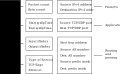
\includegraphics{figures/c02/nf5-fields}
  \end{center}
  \caption{Fields exported by NetFlow v5~\cite{CiscoSystems-2007-NetFlow}.}
  \label{fig:nf5-fields}
% http://www.cisco.com/c/dam/en/us/td/i/000001-100000/60001-65000/60001-61000/60682.ps/_jcr_content/renditions/60682.jpg
\end{figure}

NetFlow v5 was soon obsoleted by NetFlow v9 which remedied some of the deficiencies of the previous version. The state of NetFlow v9 is described in~\cite{rfc3954}. It allowed defining an arbitrary set of fields for export using templates as shown in Figure~\ref{fig:nf9-protocol}. It also introduced support for new protocols, such as IPv6, Virtual Local Area Networks (VLAN), Multiprotocol Label Switching (MPLS), Border Gateway Protocol (BGP) or Multicast. 

\begin{figure}[t!]
  \begin{center}
    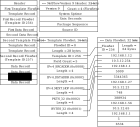
\includegraphics{figures/c02/nf9-protocol}
  \end{center}
  \caption{NetFlow~v9 protocol structure example~\cite{CiscoSystems-2007-NetFlow}.}
  \label{fig:nf9-protocol}
% http://www.cisco.com/c/dam/en/us/td/i/100001-200000/120001-130000/121001-122000/121979.ps/_jcr_content/renditions/121979.jpg
\end{figure}

Other vendors created their own versions of flow exporting protocols, although they retained some level of compatibility with NetFlow. There are JFlow by Juniper, CFlow by Alcatel-Lucent, RFlow by Ericsson, and other protocols. When the potential of flow monitoring for security purposes became realised in 2005~\cite{CiscoSystems-2005-Cisco}, more effort was devoted to extending flow records with information not directly associated with switching. Cisco presented Flexible NetFlow technology~\cite{CiscoSystems-2008-Cisco} in 2006 which allows to dynamically define and export new types of information, such as parts of payloads or traffic identification.

In 2001, it was clear that exporting flow information from switching devices was going to be supported by vendors. However, no standard flow export protocol existed at the time and NetFlow v5 was not yet released to general public. For that reason the IETF started \Index{IP Flow Information Export} (\Index{IPFIX}) WG~\cite{IETF--IP}. The original charter~\cite{IESG-2001-IP} defined six specific goals for the WG: 

\begin{itemize}
    \item Define \emph{``standard IP flow''}.
    \item Devise flow data encoding that supports multiple levels of aggregation.
    \item Allow packet sampling in IP flow.
    \item Identify and address security and privacy concerns affecting flow data.
    \item Specify the transport mapping for IP flow information.
    \item Ensure that the flow export system is reliable.
\end{itemize}

The charter was updated over the years to match current requirements. Several vendors were engaged in the IPFIX WG’s activities, most notably Cisco, which significantly contributed from the start. The WG defined a set of requirements for the IPFIX protocol~\cite{rfc3917} and evaluated existing candidate protocols~\cite{rfc3955} to decide the most suitable approach to defining the new protocol. The NetFlow v9 specification (RFC 3954) was designed with IPFIX requirements in mind~\cite{Trammell-2011-Introduction} and was released in order to compete in this evaluation (RFC 3955). After the evaluation, the NetFlow v9 was chosen as a basis of the new IPFIX protocol. For this reason, IPFIX is sometimes called NetFlow v10 and even starts with protocol version 10 in its header. However, the IPFIX protocol supports many new features and is not completely backwards compatible with NetFlow.

The IPFIX WG did more than just design the IPFIX protocol. In the 29 RFCs published before its conclusion, the WG paid attention to, e.g.:
\begin{itemize}
    \item Bidirectional flow export~\cite{rfc5103}
    \item Architecture for IP flow information export~\cite{rfc5470}
    \item Reducing redundancy in flow~\cite{rfc5473}
    \item Definitions of Managed Objects (MIB) for IPFIX~\cite{rfc5815, rfc6615, rfc8038}
    \item IP flow mediation framework~\cite{rfc5982, rfc6183}
    \item IP flow anonymization~\cite{rfc6235}
    \item IPFIX configuration data model~\cite{rfc6728}
\end{itemize}
The IPFIX protocol specification is described by \emph{``Specification of the IP Flow Information Export (IPFIX) Protocol for the Exchange of Flow Information''}~\cite{rfc7011} which became an Internet Standard. The working group was concluded in 2014, however, IPFIX related Internet-Drafts are still being created by involved parties. Further information about IPFIX development is provided by \citeauthor{Brownlee-2011-Flow} in \cite{Brownlee-2011-Flow}.

\subsection{Related Technologies}

Flow monitoring is not the only network monitoring system used to gain information about network behaviour. There are other technologies that can be used to monitor network traffic and that can sometimes be confused with flow monitoring. We describe \Index{sFlow}~\cite{Phaal-2004-sFlow}, \Index{IETF Packet Sampling}, \Index{OpenFlow} and Deep Packet Inspection\index{deep packet inspection} in the following text.

sFlow is an industry standard that is supported by a number of vendors in their packet switching devices. Its initial specification was published as an Informational RFC~\cite{rfc3176} in 2001, which was the time when packet switching/routing devices with sFlow support became available. The most crucial difference from flow monitoring is that the sFlow does not actually aggregate a stream of packets into a flow record. Instead, it uses sampling to select individual packets and then exports information available about and from these packets. sFlow allows to export data from packet headers, chunks of data from packets and even parse application payloads. It also maintains interface counters and allows their regular export, which is a feature entirely unrelated to flow monitoring. sFlow version 5 is the latest version and was published in~\citeyear{Phaal-2004-sFlow}~\cite{Phaal-2004-sFlow}.

In 2002 the IETF started Packet Sampling (PSAMP) Working Group~\cite{IETF--Packet} which was chartered to define a standard set of capabilities for network elements to sample subsets of packets by statistical and other methods~\cite{IESG--Packet}. The result is similar to sFlow; however, the PSAMP uses IPFIX protocol for data export~\cite{rfc5477}. The WG was concluded in 2009 after publishing four RFCs. The proposed standards include sampling and filtering techniques for IP packet selection~\cite{rfc5475}, packet sampling protocol specifications~\cite{rfc5476} and information model for packet sampling export~\cite{rfc5477}.

OpenFlow~\cite{ONF-2012-OpenFlow} is considered to be one of the first Software Defined Networking (SDN) standards~\cite{Singh-2017-Survey, Hu-2014-Survey}. The idea of SDN is to separate control plane and data plane of networking devices. This means that the packet forwarding rules are known only to SDN controllers. The other networking devices that process the traffic ask the controllers what to do with individual flows. After the decision is made for the first packet of the flow, a flow record is kept in the cache so that subsequent lookups do not require the controller interaction. The OpenFlow is a protocol of communication between the networking devices and the controllers. It has been shown by \citeauthor{Yu-2013-FlowSense}~\cite{Yu-2013-FlowSense} that the information stored in the flow caches can be exported using the OpenFlow protocol to the controller and used for network monitoring. Although the approach to network monitoring is somewhat similar to flow monitoring on non-SDN networking devices, there are significant differences. The control traffic itself is utilised to transfer data about new and expired flow records. Therefore, the configuration of flow monitoring is directly affected by the configuration of SDN network and vice versa. This imposes undesirable restrictions on the flow monitoring process. \citeauthor{Hendriks-2016-Assessing} assess the quality of flow data from OpenFlow devices in~\cite{Hendriks-2016-Assessing} and report numerous problems with the measurement and resulting data quality. \citeauthor{Suarez-Varela-2017-Towards} proposes a more scalable solution to mitigate some of the identified problems in~\cite{Suarez-Varela-2017-Towards}. However, the distributed architecture of the monitoring is usually tightly coupled with the deployment of the network controllers. For these reasons, this thesis does not consider SDN specific flow monitoring. It should be noted, that the SDN enabled networking devices can still export valid flow data as defined by the IPFIX standard. In any case, the SDN capabilities are irrelevant for flow monitoring purposes.

Deep Packet Inspection (DPI) is an approach to network data analysis where each packet is dissected up to and including application layer protocol (i.e. packet payload). Although this requires much higher resources than standard flow monitoring, it provides maximum information about network traffic. DPI is an approach, rather than a specific technology. Therefore the means of packet capture and information export depend on the particular deployment. For example, sFlow uses DPI to gain information about application layer from packet payloads and exports this information as part of the sFlow protocol. Despite the DPI being diametrically different to flow monitoring, it is being integrated to flow monitoring process to provide the application visibility. This merge balances the detailed view of DPI with the fast and scalable architecture of the flow monitoring. This thesis describes how the DPI is integrated to flow monitoring to create Application Flow Monitoring. Neither sFlow nor OpenFlow is discussed any further in this work and PSAMP is only mentioned as a packet sampling protocol that can be optionally applied to flow monitoring.


\section{Flow Definition}\label{sec:flow-definition}

To be able to describe the flow monitoring process accurately, we need to have a precise definition of what the flow is. The NetFlow v9 description in~\cite{rfc3954} uses the following definition:

\begin{displaycquote}{rfc3954}[Cisco Systems NetFlow Services Export Version 9]

    An IP Flow, also called a Flow, is defined as a set of IP packets
    passing an Observation Point in the network during a certain time
    interval. All packets that belong to a particular Flow have a set of
    common properties derived from the data contained in the packet and
    from the packet treatment at the Observation Point.

\end{displaycquote}

The Observation Point is defined as a location where IP packets can be observed. According to the definition, a flow is a set of packets within a particular time span. Furthermore, the packets in a flow have a set of common properties, and these properties are either derived from data contained in the packet data or from packet treatment (e.g. next hop IP address or input interface). Since this definition is quite generic, it covers most of the conventional IP flow creation techniques.

The IPFIX Protocol is an internet standard~\cite{rfc7011} with its own definition of a flow that builds upon the NetFlow v9 definition. It tries to specify what “properties derived from data contained in packet data” means and differentiates two types of data. The first is the values contained in packet headers; the second type covers the characteristics of the packet itself (e.g. packet length). The definition is as follows:

\begin{displaycquote}{rfc7011}[Specification of the IPFIX Protocol]

    A Flow is defined as a set of IP packets passing an Observation
    Point in the network during a certain time interval.  All packets
    belonging to a particular Flow have a set of common properties.
    Each property is defined as the result of applying a function to
    the values of:

    \begin{enumerate}
    \item one or more packet header fields (e.g., destination IP
        address), transport header fields (e.g., destination port
        number), or application header fields (e.g., RTP header fields
        [5]).

    \item one or more characteristics of the packet itself (e.g., number
        of MPLS labels)

    \item one or more fields derived from packet treatment (e.g., next
        hop IP address, output interface)
    \end{enumerate}
        
    A packet is defined as belonging to a Flow if it completely
    satisfies all the defined properties of the Flow.

\end{displaycquote}

Although this definition is a part of the IPFIX internet standard, there are several problems:
\begin{enumerate}
    \item It is not clear what a \emph{packet header} is. One interpretation is that it includes all protocol headers in the packet up to the packet payload (i.e. application layer). However, the transport header is mentioned explicitly, and the example indicates that it can also mean only network layer, in which case the data link layer is completely ignored.
    \item The \emph{characteristics of the packet} are not sufficiently described. One can interpret this as anything that cannot be computed directly from the packet header fields. The example states that a number of certain types of headers are considered as part of the packet's characteristics. The total packet length can also be included here (it was even used as an example in the early drafts in 2002).
    \item The IPFIX standard limits the definition of flows only to IP traffic. 
    However, flows are often created with the use of link layer headers. Moreover, the flow concept works even for non-IP connections, e.g. in technological networks. Therefore, the generic flow definition should allow even non-IP packets. It should be noted that the NetFlow v9 definition of flow explicitly defines IP flows, not generic flows.
    \item Flows using transport header fields cannot be correctly defined for fragmented IP packets, since transport layer information is present only in the first packet fragment. Both NetFlow v9 and IPFIX define a set of common properties used to decide which flow the packet belongs to. This must be derived only from the single packet, which is not possible in case of fragmented packets.
\end{enumerate}

In order to provide the complete definition of flow, we must address all the above-mentioned issues. The most direct solution is to start with the NetFlow v9 definition, allow non-IP packets and be clearer about deriving data from previous packets of the same flow which is used for correctly handling the packet fragmentation. Therefore, the definition used in this thesis is as follows:

\begin{definition}\label{def:flow}

    A \emph{\Index{flow}} is defined as a sequence of packets passing an \emph{observation point}
    in the network during a certain time interval. All packets that belong
    to a particular \emph{flow} have a set of common properties derived from
    the data contained in the packet, previous packets of the same \emph{flow},
    and from the packet treatment at the \emph{observation point}.

\end{definition}

There are two more terms connected to flow that need to be defined: \emph{flow key} and \emph{flow record}. The IPFIX definition of the Flow Key needs to be adapted to our definition of flow. We can conveniently shorten the definition to the following:

\begin{definition}\label{def:flow-key}

    A \emph{flow key} is a set of common properties that is used to specify a~\emph{flow}.

\end{definition}

A flow record is basically a tuple containing the flow key and other properties measured for the flow. Moreover, we allow inclusion of more information about the flow that is derived from external sources. An example can be a name of a user to which particular IP address belonged at the time of measurement. The following definition reflects that:

\begin{definition}\label{def:flow-record}

    A~\emph{\Index{flow record}} is a tuple which describes a particular \emph{flow} containing values of:

    \begin{enumerate}
        \item the \emph{flow key} used to specify the \emph{flow},
        \item other properties of the \emph{flow} derived from:
        \begin{enumerate}
            \item data contained in the packets of the \emph{flow},
            \item the packet treatment of the \emph{flow} at the \emph{observation point},
            \item external source of information.
        \end{enumerate}
    \end{enumerate}

\end{definition}

To make the definitions above clearer, we provide an example of real properties that might be contained in a flow record in Table~\ref{tab:flow.properties}. The table shows examples of flow record properties that can be derived from packet data and packet treatment. The properties can be aggregated when the derived value differs between individual packets of the flow or where counters such as the number of packets are involved. A~summation function is usually applied to the number of bytes in each packet, TCP flags are aggregated using a logical OR function, the flow start timestamp is derived using a minimum function on each packet timestamp. The non-aggregated properties may be used as part of a flow key.

The definition of flow record states that each flow record describes a particular flow. Moreover, in the rest of this thesis, we make the assumption that each flow is described by a single flow record. This is particularly important for long-lived flows that are terminated by an active timeout. Either the whole flow can be terminated and a new one started, or the flow can continue and only the matching flow record can be expired. Multiple flow records are created in the latter case. We use the former interpretation since it allows to simplify the following definitions.

\begin{table}[ht!]
    \centering
    \begin{tabular}{lll}
    \toprule
                                               & \textbf{Aggregated properties}  & \textbf{Non-aggregated properties}  \\ \midrule
    \multirow{3}{*}{\textbf{Packet data}}      & Number of bytes                 & Source IP address                   \\ 
                                               & TCP flags                       & Destination port                    \\ 
                                               & Time to Live                    & Transport protocol                  \\ \midrule
    \multirow{2}{*}{\textbf{Packet treatment}} & Number of packets               & Input interface number              \\ 
                                               & Flow start timestamp            & Next-Hop IP address                 \\ \bottomrule
    \end{tabular}
    \caption{Examples of Flow Properties}
    \label{tab:flow.properties}
\end{table}

Definition~\ref{def:flow} states what the flow is. Although we tried to be as explicit as possible, the definition uses informal language and is therefore subject to different interpretations. For this reason, we now provide a formal definition of flow, which not only refines the informal definition but also provides a guide to the construction of the flows.

\begin{defn}
Let $P$ be a set of all packets. Let $T$ be a set of packet treatment information. We define a set of \Index{extended packets}
\begin{equation*}
    \widehat{P} = P\times T,
\end{equation*}
so that $\widehat{p} \in \widehat{P}$ denotes a packet $p$ together with its packet treatment information. Let $\mathbb{S}$ be a set of indexes of packets observed at an \emph{observation point}:
\begin{equation*}
    \mathbb{S} = \{1, \ldots, n\}, %\lor \mathbb{N},
\end{equation*}
where $n \in \mathbb{N}$ is the number of observed packets.% when the number is finite.

We denote a sequence of packets and extended packets observed at an \emph{observation point} respectively:
\begin{align*}
    \mathcal{P} &= (p_i)_{i \in \mathbb{S}},\, p_i \in P,\\
    \widehat{\mathcal{P}} &= (\widehat{p}_i)_{i \in \mathbb{S}},\, \widehat{p}_i \in \widehat{P}.
\end{align*}
\end{defn}
Both sequences are of size $|\mathbb{S}|$. 

Let us now define a \emph{\Index{flow selection function}} $\varphi$ which takes a sequence of extended packets and a new extended packet and decides whether they form a flow. We will use this function to determine whether a newly observed packet belongs to an existing flow.
\begin{defn}\label{def:flow-selection-function}
Let $\widehat{P}^*$ be a set of all finite sequences of extended packets, $\widehat{P}$ be a set of extended packets. We say that a function of type
\begin{equation*}
    \varphi: \widehat{P}^*\times \widehat{P} \to \{\mli{true,false}\}
\end{equation*}
is a \emph{flow selection function}.
\end{defn}

Before we give a formal definition of a flow\index{flow!formal definition of}, we provide the following intuition for our definition. A flow $\mathcal{F}$ is a sequence of packets defined by a sequence of extended packets with indexes in $\mathbb{S}$ and a \emph{flow selection function} $\varphi$. We require that a packet belong to a flow if it is determined by all previous packets of that flow. Therefore we construct the flow by induction as described in Algorithm~\ref{alg:flow-construction}.

\begin{algorithm}
    \caption{Construction of a flow}
    \label{alg:flow-construction}
    \begin{algorithmic}[1]
        \STATE Denote $\mathbb{I}$ the set of packet indexes that belong to the flow $\mathcal{F}$
        \STATE Start with $\mathbb{I} = \emptyset$
        \WHILE{An index $k$ of the first extended packet $\widehat{p}_k$ for which $\varphi((\widehat{p}_n)_{n\in \mathbb{I}},\, \widehat{p}_k) = \mli{true}$ exists}
            \STATE Add $k$ to $\mathbb{I}$
        \ENDWHILE
        \STATE The flow $\mathcal{F}$ is a sequence of packets with indexes from $\mathbb{I}$
    \end{algorithmic}
\end{algorithm}

We shall now define set $\mathbb{I}$ of indexes from $(\widehat{p}_i)$ selected using \emph{flow selection function} $\varphi$, and flow $\mathcal{F}$ so that it conforms with the Definition~\ref{def:flow} as follows:
\begin{defn}\label{def:formal-flow}
Let $(p_i)_{i \in S}, (\widehat{p}_i)_{i \in S}, S \subseteq \mathbb{S}$ be %(possibly finite)
mutually corresponding sequences of packets and extended packets respectively, $\varphi$ a \emph{flow selection function}.

We define a \emph{flow index set} $\mathbb{I} = \mathbb{I}\left((\widehat{p}_i)_{i \in S},\, \varphi\right)$ as 
\begin{align*}
\mathbb{I} &= \bigcup_{i \to \infty} J_i \text{, where } J_i \text{ is defined inductively over }i \in \mathbb{N} \text{ as:} \notag\\
J_i &= \left\{
    \begin{array}{ll}
        \left\{\min\left\{ \alpha \in S \mid \varphi(\widehat{p}_{\alpha}) = \mli{true} \right\}\right\} & \text{for } i = 1 , \\[0.7em]
        J_{i-1} \cup \{\min\{ \alpha \in S \mid \alpha > \max(J_{i-1}), & \multirow{2}{*}{\text{for } $i > 1$.} \\
        \quad \varphi((\widehat{p}_n)_{n\in J_{i-1}},\, \widehat{p}_{\alpha}) = \mli{true} \}\} &
    \end{array}\right.
\end{align*}

Finally, we define flow $\mathcal{F} = \mathcal{F}\left((p_i)_{i \in S},\, \mathbb{I}\right)$ as:
\begin{equation*}
    \mathcal{F} = (p_i)_{i \in \mathbb{I}},\, p_i \in \mathcal{P}.
\end{equation*}

\end{defn}

Since we need the $\min$ function to be defined for an empty set (the cases where no flow is defined and where we have already added all possible indexes from $\mathbb{S}$), we define
\begin{equation*}
    \left\{\min\ \emptyset \right\} = \emptyset
\end{equation*}

Definition~\ref{def:formal-flow} of flow creates a single flow for a sequence of extended packets $\widehat{\mathcal{P}}$ and a \emph{flow selection function} $\varphi$. The flow $\mathcal{F}$ is selected based on the first extended packet accepted by $\varphi$. Since we naturally expect that every packet is a part of only a single flow, we can construct a sequence of flows $(\mathcal{F}_i)_{i \in \mathbb{N}}$ by induction as described in Algorithm~\ref{alg:flow-sequence-construction}.

\begin{algorithm}
    \caption{Construction of a sequence of flows}
    \label{alg:flow-sequence-construction}
    \begin{algorithmic}[1]
        \STATE Denote $S_1 = \mathbb{S}$
        \STATE Set counter $i = 1$
        \REPEAT
            \STATE Apply the \emph{flow selection function} $\varphi$ to extended packets with indexes in $S_i$
            \STATE Denote indexes of matching extended packets $\mathbb{I}_i$
            \STATE Flow $\mathcal{F}_i $ is a sequence of packets with indexes from $\mathbb{I}_i$
            \STATE Remove indexes in $\mathbb{I}_i$ from $S_i$, denote the new sequence $S_{i+1}$
            \STATE Increment counter $i = i + 1$
        \UNTIL{$\mathcal{S}_i$ is empty}
    \end{algorithmic}
\end{algorithm}

Let us now provide a more formal definition of a sequence of flows $(\mathcal{F}_i)_{i \in \mathbb{N}}$.
\begin{defn}\label{def:formal-flow-sequence}
Let $\mathcal{P}, \widehat{\mathcal{P}}$ be sequences of packets and extended packets respectively, $\varphi$ a \emph{flow selection function}. We define the sequence $(\mathcal{F}_i)_{i \in \mathbb{N}}$ of flows inductively:
\begin{align*}
    \mathcal{F}_i &= \mathcal{F}_i\left((p_j)_{j\in S_i},\, \mathbb{I}_i\right) \text{, where} \\
    S_1 &= \mathbb{S}, \\
    S_i &= S_{i-1} \setminus \mathbb{I}_{i-1}, \\
    \mathbb{I}_{i} &= \mathbb{I}_i\left((\widehat{p}_j)_{j \in S_i},\, \varphi\right).
\end{align*}
\end{defn}

Definition~\ref{def:formal-flow-sequence} provides a guide to constructing a sequence of flows. The procedure can be easily modified to run in real time so that each newly observed extended packet can be added to the appropriate flow. In our definition, we want every packet to be a part of only a single flow. Therefore, we apply the \emph{flow selection function} $\varphi$ to each pair of existing flow (enriched by packet treatment information) and the new extended packet. Then, we add the packet to the first flow that matches. If none of the existing flows matches, we apply the function $\varphi$ to this packet only and start a new flow if necessary. 

From this, we can see that the flow creation process depends solely upon the implementation of the \emph{flow selection function}. We will shortly discuss common implementations in the Subsection~\ref{subsec:flow-creation}.

The condition for every packet to be part of exactly one flow might be too constricting in some cases. It is possible to remove the condition and simply start building each flow from a next extended packet in the sequence. However, this will create many overlapping flows that contain mostly the same packets but start with a different one. This problem would need to be addressed should such a definition be used.

\section{Flow Monitoring Architecture}\label{sec:flow-monitoring-architecture}

Deployment of flow monitoring on a network requires several steps: Capturing packets at one or more observation points, assigning packets to flows, creating and exporting flow records for the flows, and finally collecting, storing, and processing of the exported flow records. 
The Figure~\ref{fig:flow-monitoring-process} shows a high-level overview of the whole process. Flow monitoring process encompasses packet capture, flow creation, and creation and export of flow records. Flow data processing comprises of flow record collection, storage, and further processing. Note that the flow records can be processed directly without storing. This approach is called \emph{stream processing}. It is also possible to manipulate the flow records in transition between the export and collection. The IPFIX working group specified a framework called IP Flow Information Export Mediation~\cite{rfc6183} which describes this process. However, description of this process is outside the scope of this thesis.

\begin{figure}[t!]
  \begin{center}
    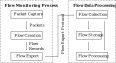
\includegraphics{figures/c02/flow-monitoring-process}
  \end{center}
  \caption{High Level Flow Monitoring Schema}
  \label{fig:flow-monitoring-process}
\end{figure}

This rest of section explains basic terminology and components of the flow monitoring architecture and describes the most commonly deployed flow monitoring architectures.

\subsection{Terminology}

The IPFIX working group published several documents where the architecture for IP Flow Information Export is described~\cite{rfc5470, rfc6183}. However, the terminology used in these documents is not commonly used by the flow monitoring community, and some of the terms have different meaning depending on a context. We start by presenting the IPFIX reference model as described in RFC5470~\cite{rfc5470}, which can also be used to describe generic flow monitoring architecture. Then we identify the terms that are often used with different meaning and explain how these terms are used throughout this thesis.

We provide the IPFIX terminology definitions from RFC 7011~\cite{rfc7011} here for the convenience of the reader:

\begin{displaycquote}{rfc7011}[Specification of the IP Flow Information Export (IPFIX) Protocol for the Exchange of Flow Information]

    \begin{description}[style=nextline]
        \item[Observation Point]
      An Observation Point is a location in the network where packets
      can be observed.  Examples include a line to which a probe is
      attached; a shared medium, such as an Ethernet-based LAN; a single
      port of a router; or a set of interfaces (physical or logical) of
      a router.

      Note that every Observation Point is associated with an
      Observation Domain (defined below) and that one Observation Point
      may be a superset of several other Observation Points.  For
      example, one Observation Point can be an entire line card.  That
      would be the superset of the individual Observation Points at the
      line card's interfaces.
      
        \item[Observation Domain]
      An Observation Domain is the largest set of Observation Points for
      which Flow information can be aggregated by a Metering Process.
      For example, a router line card may be an Observation Domain if it
      is composed of several interfaces, each of which is an Observation
      Point.  In the IPFIX Message it generates, the Observation Domain
      includes its Observation Domain ID, which is unique per Exporting
      Process.  That way, the Collecting Process can identify the
      specific Observation Domain from the Exporter that sends the IPFIX
      Messages.  Every Observation Point is associated with an
      Observation Domain.  It is RECOMMENDED that Observation Domain IDs
      also be unique per IPFIX Device.

        \item[Packet Treatment]
      "Packet Treatment" refers to action(s) performed on a packet by a
      forwarding device or other middlebox, including forwarding,
      dropping, delaying for traffic-shaping purposes, etc.

        \item[Metering Process] 

      The Metering Process generates Flow Records.  Inputs to the
      process are packet headers, characteristics, and Packet Treatment
      observed at one or more Observation Points.

      The Metering Process consists of a set of functions that includes
      packet header capturing, timestamping, sampling, classifying, and
      maintaining Flow Records.

      The maintenance of Flow Records may include creating new records,
      updating existing ones, computing Flow statistics, deriving
      further Flow properties, detecting Flow expiration, passing Flow
      Records to the Exporting Process, and deleting Flow Records.
      
        \item[Exporting Process]
      The Exporting Process sends IPFIX Messages to one or more
      Collecting Processes.  The Flow Records in the Messages are
      generated by one or more Metering Processes.

        \item[Exporter]
      A device that hosts one or more Exporting Processes is termed an
      Exporter.

        \item[IPFIX Device]
      An IPFIX Device hosts at least one Exporting Process.  It may host
      further Exporting Processes as well as arbitrary numbers of
      Observation Points and Metering Processes.

        \item[Collecting Process]
      A Collecting Process receives IPFIX Messages from one or more
      Exporting Processes.  The Collecting Process might process or
      store Flow Records received within these Messages, but such
      actions are out of scope for this document.

        \item[Collector]
      A device that hosts one or more Collecting Processes is termed a
      Collector.
    \end{description}

\end{displaycquote}


The Figure~\ref{fig:ipfix_reference_model} shows various scenarios of flow monitoring architecture as defined by IPFIX working group. IPFIX exporters and IPFIX devices are part of the flow monitoring process, collectors and application represent flow data processing, as described in the Figure~\ref{fig:flow-monitoring-process}. The IPFIX Reference Model~\cite{rfc5470} allows differentiating between devices that only export flow records and devices that receive data from an observation point and perform the metering process themselves. This can be useful for describing for example development setups where flow records are replayed or generated without the necessity for monitoring of live network traffic. Collectors comprise of collecting processes and data processing applications. The reference model shows that it is possible to collect flow records from multiple sources on a single collector and that the applications can run directly on the collector or that they can be distributed to other machines. For example, collecting process might convert the flow records in IPFIX format to JSON and feed a big data processing framework that runs on a cluster of machines.

\begin{figure}[t!]
  \begin{center}
    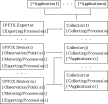
\includegraphics{figures/c02/ipfix-reference-model}
  \end{center}
  \caption{IPFIX Reference Model~\cite{rfc5470}}
  \label{fig:ipfix_reference_model}
\end{figure}

Although the IPFIX Reference Model describes the flow monitoring architecture in detail, it is not used by the flow monitoring community unanimously. Most of the terms used in the IPFIX standard are simplified, and their true meaning often depends on the context. Table~\ref{tab:flow_monitoring_terminology} provides the common terms often used instead of the IPFIX terminology. Examples of the use of the \Index{common terminology} can be found for example in~\cite{Hofstede-2014-Flow, Cejka-2015-Using, Brownlee-2011-Flow, Krmicek-2009-Netflow, Lee-2007-End, Lee-2007-IPv6, Molina-2006-Design}. We usually talk about a monitored link and a set of monitored links (e.g. both directions of a network connection when optical fibres are used) instead of an observation point or an observation domain. By an exporter or a flow exporter is usually meant the software that performs flow monitoring (both metering and exporting process). If a device generates flows without observing and processing the packets first (i.e. Exporter in IPFIX terminology), we call it a flow source or a probe. The IPFIX Device is usually called by more specific name, such as a switch, router, or, in case of a dedicated device possibly with specialised hardware and software equipment, a probe. Furthermore, the term flow source can also be used for any device that generates flow records. Finally, both the software for collecting flow records and device where such software runs is commonly called a collector, or a flow collector. We will be using the common terminology throughout this thesis.

\begin{table}[t!]
    \centering
    \begin{tabular}{ll}
    \toprule
        \textbf{IPFIX Terminology}  & \textbf{Common Terminology}                 \\ \midrule
        Observation Point   &  Monitored Link, Observed Link                      \\
        Observation Domain  &  Set of Monitored Links                             \\
        Packet Treatment    &  Packet Treatment                                   \\
        Metering Process    &  (Flow) Exporter [software]                         \\
        Exporting Process   &  (Flow) Exporter [software]                         \\
        Exporter            &  Flow Source, (Flow) Probe                          \\
        IPFIX Device        &  Flow Source, (Flow) Probe, Switch, Router, \ldots  \\
        Collecting Process  &  (Flow) Collector [software]                        \\
        Collector           &  (Flow) Collector [device]                          \\ \bottomrule
    \end{tabular}
    \caption{Flow Monitoring Architecture Terminology}
    \label{tab:flow_monitoring_terminology}
\end{table}


\subsection{Flow Monitoring Deployment}

The deployment of flow monitoring requires careful planning so that it does not disturb the existing network infrastructure. There are several decisions that must be made such as choosing a proper flow source, collector and their location relative to the monitored network. Although it is possible to monitor wireless and virtual networks, we focus on the deployment in wired networks.

The selection of the flow source depends upon many variables, such as cost, required quality of exported data, or the type of the monitored link. Two types of flow source are generally available. First are the active networking devices that are already present in the network and provide flow monitoring functionality as well. Switches, routers and firewalls belong to this category. When such a device is present at a convenient point in the network, it is sufficient to configure it for flow export, and no adjustments to the network are needed. Moreover, internal information such as IP addresses behind NAT (Network Address Translation), which would be difficult to access otherwise, can be added to exported flow records. The disadvantage of these devices is that flow monitoring is not their primary function and may not be performed correctly under high load (i.e. under certain types of attack). Also, the range of supported options and protocols is usually much lower than that of dedicated probes. The reason for deploying a dedicated probe is usually the need for some extra functionality or guarantees that cannot be met by the networking devices. Furthermore, it allows separating network configuration and maintenance from network monitoring, which can be useful if they are handled by different divisions of an organisation.

The active networking devices observe packets as a part of their function, dedicated probes, however, need to be provided with access to data. There are two ways for probes to observe the data: in \emph{in-line} mode or \emph{mirrored} mode.
\begin{description}
    \item[In-line mode] -- A device in in-line mode is connected directly to the monitored link and has to actively pass the packets in order for the link to function. This is the mode of operation of active network devices such as switches and routers. The advantage is that no other device is necessary to mirror the traffic, however, if the probe fails the operation of the network is disrupted. Moreover, it could introduce significant latency and jitter to the network connection.
    \item[Mirrored mode] -- In the mirrored mode, a copy of network traffic is created and delivered to the probe using a dedicated link. The copy can be created either by dedicated TAP (Test Access Point) or an active networking device with the use of a SPAN (Switch Port Analyzer) port. Table~\ref{tab:tap_vs_span} shows differences, advantages, and disadvantages of TAP and SPAN solutions. An analysis of traffic trace artefacts caused by port mirroring was performed by~\citeauthor{Zhang-2007-Traffic} in~\cite{Zhang-2007-Traffic}.
    \begin{description}
        \item[TAP] is a passive splitting mechanism which requires in-line installation. However, due to the simplicity of the device (optical TAPs use mirrors and require no power source) and integrated fail-safes (bypass TAPs), the risk of negatively affecting the network is very low. 
        \item[SPAN] is a special port provided by active networking device that provides a copy of traffic passing through the device for analysis and monitoring purposes.
    \end{description}
\end{description}

\begin{table}[t!]
    \centering
    \begin{tabularx}{\textwidth}{XX}
    \toprule
        \multicolumn{1}{c}{\textbf{TAP}}  & \multicolumn{1}{c}{\textbf{SPAN}} \\ \midrule[1pt]
        
        \multicolumn{2}{c}{Differences} \\ \midrule
        \begin{compactitem}
            \item RX \& TX signal delivered on separate ports
            \item Captures everything on the wire, including MAC and media errors
            \item Complete capture for 100\,\% saturated network
        \end{compactitem}
        &
        \begin{compactitem}
            \item RX \& TX copied into in one TX signal
            \item Hardware and media errors are dropped
            \item Possible packet drop due to SPAN link capacity limit
        \end{compactitem}
        \\ \midrule
        
        \multicolumn{2}{c}{Advantages} \\ \midrule
        \begin{compactitem}
            \item Monitoring device receives identical data, including errors
            \item Keeps link directions separate
        \end{compactitem}
        & 
        \begin{compactitem}
            \item Low cost 
            \item No changes to network topology
            \item Aggregation of multiple links
        \end{compactitem}
        \\ \midrule
        
        \multicolumn{2}{c}{Disadvantages} \\ \midrule
        \begin{compactitem}
            \item Analysis device may need dual-port capture interface
            \item Additional costs for TAP
            \item Necessity to install additional device
        \end{compactitem}
        & 
        \begin{compactitem}
            \item Packet drop on fully utilized full-duplex links
            \item SPAN port data has lower priority than port-to-port data
            \item Some analyses require observation of physical layer errors
            \item Loss of information about link
            \item Increased switch CPU utilization
            \item Can change a timing of frames
        \end{compactitem}
        \\ \bottomrule
    \end{tabularx}
    \caption{Differences Between TAP and SPAN Mirroring Options.}
    \label{tab:tap_vs_span}
\end{table}

Since flow monitoring is a passive form of monitoring in its nature, it is a good practice to mirror the live traffic and provide only a copy of the data to the probe so that the network cannot be affected by the monitoring process. Selection of the mirroring technology needs to be considered for each deployment based on specific requirements and limitations, such as utilisation of the measured network and impact of packet drop on the performed analysis. The Figure~\ref{fig:flow_monitoring_deployment} shows the most common deployment of flow monitoring at the edge of the network using both presented options: flow export directly from the router and dedicated probe with data provided either by TAP or by router SPAN port.

\begin{figure}[t!]
  \begin{center}
    
\includegraphics{figures/c02/flow-monitoring-deployment}
  \end{center}
  \caption{Flow Monitoring Deployment Schema}
  \label{fig:flow_monitoring_deployment}
\end{figure}

Location of the flow source in the network is essential. When the monitored network is connected to the outside at multiple points, it is necessary not only to monitor each of the points but also to be sure that the routing policies are reasonable, so that packets of each flow traverse only one of these points. The flow source would have to have access to all links and monitor them as a single source otherwise, which is not easily achieved, especially when the connection points are geologically distributed. It is a good practice to keep the information about which flow source exported which flow records on the collector in order to detect possible configuration problems more efficiently.

When monitoring a large network such as a network of a university campus, multiple flow sources can be utilised to gain more detailed information about traffic of individual faculties. Special care needs to be taken when a packet traverses multiple observation points. Counting the same traffic multiple times can have a negative impact on subsequent data analysis.

Deployment of NAT impedes network visibility. Some routers that perform the address translation are able to export both original and translated addresses in the flow records. However, observation points of dedicated flow probes are located either before or after the network device which performs the translation. Although some effort has been dedicated to detection of NAT from data provided in flow records~\cite{Abt-2013-Passive, Krmicek-2009-Netflow}, it does not solve the problem of finding the correct source of the communication behind the NAT. The correct approach would be to either place a second probe to a location where the internal addresses are still visible or to export the information about translation to the collector and pair it with existing flow records.


\section{Flow Monitoring Process}\label{sec:flow-monitoring-process}

This section aims to describe the process of converting raw packets and corresponding packet treatment information to flow records. We show how the flow selection function from Definition~\ref{def:flow-selection-function} relates to this process. For the purposes of this thesis, we will consider dedicated probes equipped with a flow exporter software from now on. Although the flow monitoring process in networking devices is similar, it has differences and specifics that are outside the scope of this work. This section provides a generic overview of the flow monitoring process, and performance related details are left for Chapter~\ref{chap:flow-monitoring-performance}.

The Figure~\ref{fig:flow_monitoring_process_detail} shows a common flow monitoring process and its individual parts, which are discussed in the rest of this section. An alternative description of the flow monitoring process can be found in the IPFIX Reference Model~\cite{rfc5470}. We will refer to this description where appropriate.

\begin{sidewaysfigure}
  \begin{center}
    \includegraphics{figures/c02/flow-monitoring-process-detail}
  \end{center}
  \caption{Detailed Overview of the Flow Monitoring Process in a Dedicated Probe}
  \label{fig:flow_monitoring_process_detail}
\end{sidewaysfigure}

\subsection{Packet Capture}

The \Index{packet capture} ensures that data from the network are made available for processing in the software. Standard Network Interface Cards (NICs) can be used, as well as specialised hardware-accelerated cards. The schema shows a standard NIC performing a CRC check on received packets. The NIC has to be put in a special monitoring mode in order to receive packets with different destination MAC addresses. These packets are passed to the NIC driver, usually through Direct Memory Access (DMA). The driver either passes the received packets to the operating system or provides its own application interface for accessing the packets from user space. The performance of the different approaches differ significantly, and we will discuss it in Chapter~\ref{chap:flow-monitoring-performance} in detail.

Each packet needs to be assigned a (preferably unique) timestamp that marks the point in time at which the packet was received. This process is called packet timestamping. The timestamp can be assigned by the NIC, NIC's driver (or OS), or the software application processing the packet. The support for NIC timestamping is provided by some of the hardware-accelerated NICs. As the timestamping in software can be potentially computationally intensive, we will also discuss it in Chapter~\ref{chap:flow-monitoring-performance}.

The packet treatment information is provided together with the packets by the NIC's driver. Usually, the interface of NIC on which the packet was captured and the timestamp of the capture is available at least. Networking devices can provide more information such as egress interface, next hop, or autonomous system number of the destination. This information is not directly available when dedicated probes are used, but can be added externally if necessary.

\subsection{Packet Processing}\label{subsec:packet-processing}

The task of the \Index{packet processing} is to extract values of chosen properties of individual packets and corresponding packet treatment information. Attributes such as IP addresses, transport protocol, and ports are used as \emph{flow keys}. The set of used flow keys depend on the applied flow selection function which is used to decide to which flow the packet belongs to. Other attributes of the packets such as TCP flags or the number of bytes are extracted as well for further analysis. We call the extracted properties \emph{\Index{packet metadata}} or \emph{\Index{partial flow records}}. The packet metadata are passed to flow creation part of the flow processing where it is used to create new or update existing flow records.

Secondary task of packet processing is packet sampling and packet filtering, as mentioned in~\cite{rfc5470}. Packet sampling is usually done to reduce the amount of processed data in order to compensate for lack of performance. There are several sampling techniques that can be used as described in~\cite{rfc5476}. Packet sampling is performed before extracting the metadata. Packet filtering can be performed after the metadata is extracted and is based on the extracted values. It is common to monitor only specific network or a section of the network; therefore the filtering rules are usually based on extracted IP addresses. Both packet sampling and packet filtering can be implemented in hardware-accelerated NICs as well.

\subsection{Flow Creation}\label{subsec:flow-creation}

The extracted packet metadata are aggregated to create flow records. The definition of the flow selection function requires all preceding extended packets of the same flow to determine whether a new packet belongs to the particular flow. Since it is not viable to keep all packets of a flow in memory, only selected information is stored in real-world implementations. All active flows have a flow record with all the necessary information stored in a \emph{\Index{flow cache}}. When a new packet arrives, the flow selection function is called for each stored flow record and the metadata of the new packet to determine, to which flow the new packet belongs. If a matching flow record is found, it is updated using the packet metadata (e.g. packet and byte counters are incremented, and the flow end timestamp is updated). If no such record exists, the packet is considered to be the first packet of a new flow and a corresponding flow record is created in the flow cache. Algorithm~\ref{alg:flow-record-construction} illustrates the flow creation process. It is worth noting that the flow selection function is denoted $\phi$ as we refer to a concrete implementation here instead of the formal definition.

\begin{algorithm}
    \caption{Construction of flow records}
    \label{alg:flow-record-construction}
    \begin{algorithmic}[1]
        \LOOP 
            \STATE Get new packet $P$
            \STATE Extract packet metadata $M$
            \STATE Set \textbf{found} = \FALSE
            \FORALL{flow record $\mathcal{F}$ in flow cache}
                \STATE Apply flow selection function $\phi$ to $\mathcal{F}$ and $M$
                \IF{$\phi(\mathcal{F}, {M}) = \mli{true}$}
                    \STATE Aggregate $M$ to $\mathcal{F}$
                    \STATE Set \textbf{found} = \TRUE;
                    \STATE \textbf{break}
                \ENDIF
            \ENDFOR
            \IF{\NOT found}
                \STATE Create new flow record $\mathcal{F}$ from $M$
                \STATE Insert $\mathcal{F}$ into flow cache
            \ENDIF
        \ENDLOOP
    \end{algorithmic}
\end{algorithm}

Testing the extracted packet metadata against each flow record has a linear time complexity with respect to the size of the flow cache. A common optimisation is to compute a hash for each flow record such that it can also be computed for the extracted metadata. The flow cache is then either indexed by using the computed hash~\cite{Molina-2006-Design} or directly implemented as a hash table~\cite{Estan-2004-Building} so that the input and lookup operations have a constant time complexity. Collisions can be solved by a number of common techniques or by prematurely exporting the older colliding flow record. This optimisation is so widely used that its use is often implicit, but it is important to keep in mind that the new packet is still effectively tested against each active flow. Other implementations of flow caches can be found in literature, such as a hypercube flow table by~\citeauthor{Wang-2011-Memory}~\cite{Wang-2011-Memory}.

There are several reasons why a flow record can exit the flow cache\index{flow!record expiration}{}:
\begin{description}
    \item[Inactive timeout\index{timeout!inactive}] occurs when no new packets belonging to the flow arrive for a time interval called \emph{inactive timeout}. This timeout is used to end inactive connections and has a significant influence on flow cache memory requirements. When set too low the inactive timeout can erroneously split idle connections where keep-alive packets are sent in a longer interval than the inactive timeout. The inactive timeout is sometimes called \emph{idle timeout}\index{timeout!idle} as well.
    \item[Active timeout\index{timeout!active}] occurs when the flow is longer than a time interval called \emph{active timeout}. The reason for active timeout is to keep exported flow information fresh. For example, some SSH connections may be active for months when left open in a UNIX/Linux screen utility, and without the active timeout, the information about the connection would be too late for any practical purpose, such as monitoring the amount of traffic for a given time period. The active timeout is usually much longer than the inactive one. For example, Cisco IOS flow cache has the default of 30 minutes for the active timeout and 15 seconds for the inactive one~\cite{CiscoSystems-2013-Cisco}.
    \item[Natural expiration] occurs when the connection is closed normally. This is often implemented for TCP connections where packets with RST or FIN flag indicate the end of the connection.
    \item[Resource constraints] such as lack of memory can cause flow records to be exported from the flow cache to allow new flows to be inserted. Some implementations of flow caches using hash tables have fixed number of flows that can be stored under single hash. Therefore, when a new flow record needs to be created, one of the existing flow records is usually expired.
    \item[Exporter shutdown] usually causes all flow records in the flow cache to be exported so that the information about observed packets is not lost. This cause is not often mentioned in the literature; however, we consider it an important one. The exporter must be restarted each time a configuration is changed unless it supports dynamic reconfiguration, which none of the open-source exporters does. Therefore the exported shutdown can happen surprisingly often.
\end{description}

The RFC 5470~\cite{rfc5470} considers both timeouts and resource constraints as causes for a flow record to expire but omits natural close of connection and the possibility of exporter shutdown. Flow record expiration setting can significantly influence not only the number of generated flow records, as shown by the authors of~\cite{Rodriguez-2013-Empirical}, but also further flow processing and various flow-based detection methods. Implementation of flow record expiration has an impact on the overall flow monitoring performance. Periodically checking the flow cache for expired flows can create latency in packet capture that may result in packet loss. Several approaches to this problem are described in the work of \citeauthor{Molina-2006-Design}~\cite{Molina-2006-Design}.

% On the impact of TCP segmentation: Experience in VoIP monitoring by D. Muelas et al.; and Low-cost and high-performance: VoIP monitoring and full-data retention at multi-Gb/s rates using commodity hardware, by J.L. García-Dorado et al. 
% Both works cope with this matter and provide some insights that may extend the discussion in the manuscript.

Little attention has been given to the measurement of traffic with fragmented packets. Although the ratio of fragmented packets is decreasing~\cite{Murray-2012-State}, it is still vital to monitor them since it is quite easy for an attacker to hide an attack from intrusion detection systems by fragmenting the attack packets~\cite{Cheng-2012-Evasion}. The RFC 3917 which describes requirements for IP flow information export states the following about packet fragmentation:

\begin{displaycquote}{rfc3917}[Requirements for IP Flow Information Export (IPFIX)]
   In case of IP packet fragmentation and depending on the
   classification scheme, only the zero-offset fragment of a single
   initial packet might contain sufficient information to classify the
   packet.  Note that this fragment should be the first one generated by
   the router imposing the fragmentation [RFC791], but might not be the
   first one observed by the IPFIX device, due to reordering reasons.
   The metering process may keep state of IP packet fragmentation in
   order to map fragments that do not contain sufficient header
   information correctly to flows.
\end{displaycquote}

This means that the flow monitoring system implementing the IPFIX standard is not required to handle fragmented packets. Moreover, neither the Netflow v9 nor the IPFIX flow definitions cover the possibility to assign a packet fragment to the correct flow, because they require the common properties to be derived from the single packet and the corresponding packet treatment. This is the main reason that the Definitions~\ref{def:flow} and~\ref{def:formal-flow} allow to derive the common properties from data contained in previous packets of the same flow as well. We assume that the packets arrive in the appropriate order for the purpose of these definitions.

Let us consider what happens when an IPv4 packet is fragmented (the problem is very similar for IPv6). Figure~\ref{fig:fragmented-flow} illustrates this scenario. When the packet $K$ is fragmented, its payload is distributed between several different packets $(K\#1, K\#2, \ldots, K\#M_K)$. Only the first packet $(K\#1)$ contains the transport header; others only carry a flag identifying the fragment and offset of the data in the original packet. When a flow record is created for the first part of the fragmented packet, it contains IP addresses, transport layer information (protocol and ports), and the first part of application payload. However, subsequent parts contain only information about IP addresses and consecutive parts of the application payload. The transport level information was already sent in the first fragment. Therefore, flow records created from the subsequent fragments are not aggregated with the first fragment. Moreover, flow records created from subsequent fragments from different connections between the same hosts are aggregated together. To resolve this problem, some kind of packet reassembly must happen either in the flow cache or during packet capture (e.g. packet reassembly at the OS network stack).

A possible solution that has been successfully deployed in practice is to create temporary flow records for fragmented packets where fragmentation identifiers are part of the flow key instead of transport layer information. Therefore, each fragmented packet has its own temporary flow record. By assigning shorter inactive timeout to these flow records, the temporary flow record can be reinserted into the flow cache when all fragments are received. This allows to efficiently reassemble the original packet with proper transport layer information, which is available since it was present in the first fragment, in the flow cache. The advantage of this solution is that it allows counting the number of reassembled packets as well as the number of packet fragments, which can be used in later analyses.

\begin{figure}[ht!]
  \begin{center}
    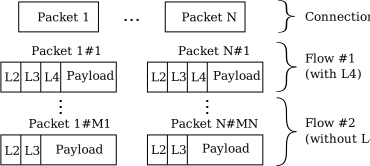
\includegraphics{figures/c02/fragmented-flow}
  \end{center}
  \caption{Flow measurement of a fragmented connection.}
  \label{fig:fragmented-flow}
\end{figure}

The flow monitoring implementation based on flow caches of networking devices kept a separate flow for each direction of a network connection. The reason was that each direction usually had different at least ingress and egress interfaces. However, for network monitoring and analysis purposes, it is often useful to be able to access flow records for both communication directions at the same time. For this reason, the bidirectional flow export was proposed in 2005 and resulted in the publication of RFC 5103~\cite{rfc5103} in 2008. The document proposes to aggregate flow records for both forward and reverse directions to a single flow record. Bidirectional flow is called \emph{\Index{biflow}} and unidirectional flow is called \emph{\Index{uniflow}}. The flow keys that are associated with a direction (e.g. source IP address) are called \emph{directional flow keys}. When the biflow record is created, some information must be stored for both directions (e.g. number of bytes and packets), and some information is common to both directions (e.g. flow keys). When biflows are used, the corresponding flow records stored in the flow cache become biflow records as well. Note that creation of biflows is permitted by the definitions NetFlow v9 and IPFIX as well as the Definition~\ref{def:flow}. Although we work mostly with the uniflow in the context of this thesis, most of the concepts apply to the biflow as well. We will explicitly mention when there are important differences between uniflow and biflow.

\subsection{Flow Export}

The flow export manages the process of delivering flow records to flow collectors. The process consists of several parts as shown in the Figure~\ref{fig:flow-export}. The flow sampling and filtering process is very similar to packet sampling and filtering described in the Subsection~\ref{subsec:packet-processing}. The primary motivation for flow filtering is that each collector might want to process only a subset of data, e.g. from a particular subnet. The flow sampling is performed when the performance of the collector is not sufficient to process all flow records. The main difference between packet sampling and flow sampling is that the flow sampling always discards whole flow record while the packet sampling can discard some packets of the flow, therefore affecting the created flow record. 

\begin{figure}[ht!]
  \begin{center}
    \includegraphics{figures/c02/flow-export}
  \end{center}
  \caption{Flow export schema.}
  \label{fig:flow-export}
\end{figure}

The flow export protocols such as NetFlow or IPFIX describe how to serialise a flow record and how to use different transport protocols such as UDP, TCP and SCTP to transfer the encoded data to the collector. The NetFlow~v5 and v9 protocols are still widely used although the IPFIX protocol is achieving wide deployment since it offers additional features and supports proprietary information elements as well as variable length information elements. Different flow export protocols developed by other vendors can be used as well, as described in Subsection~\ref{subsec:history-of-flow-monitoring}.

The UDP transport protocol is used very often to carry flow records since it was the only one supported by NetFlow. IPFIX specifies the use of TCP and SCTP protocols for flow export as well as the use of the UDP protocol. Although SCTP is mandatory for IPFIX implementations, its real-world usage is hindered by lack of support in software and hardware. When a reliable transport is necessary, TCP is the most often used protocol. For more information about IPFIX transport protocols see RFC 7011~\cite{rfc7011}. A comprehensive comparison of IPFIX transport protocols is also provided in~\cite{Hofstede-2014-Flow}.

Flow records can be exported in many formats over different transport protocols. With the increasing popularity of big data tools such as Kafka, Elasticsearch, Apache Spark, and Hadoop, the need for a universal and widely supported format is more crucial than ever before. As most of the big data tools support JSON, flow records are often transported and stored in the JSON format. The main advantage of JSON is that the data are stored in a key-value format without the need to specify templates for the data beforehand. The obvious disadvantage is the increase in the message size due to the need to provide a key for every value in every flow record. It is not unusual for the JSON encoded messages to be more than seven times larger than in the IPFIX format.

An important part of flow export is ensuring the security of the exported flow records. The records must reach only the authorised destination without being observed by any third party. Therefore, authorisation, confidentiality and, preferably, also integrity should be provided. The same applies to flow collectors during the collecting process. More information about flow transmission security is provided in Subsection~\ref{subsec:flow-collection}.

\section{Flow Data Processing}\label{sec:flow-data-processing}

The aim of this section is to outline the processing of flow data after they are exported to a flow collector. Firstly, we describe the flow collection process in Subsection~\ref{subsec:flow-collection}. The reception of flow data is not a difficult task itself but requires several important choices to be made, such as what flow export protocols will be supported and how to handle unknown information elements. Secondly, the flow data are often stored for future needs. The choice of a flow data storage format is fundamental since the data is written once, read many times and fast searches are required. This process is described in Subsection~\ref{subsec:flow-storage}. Lastly, the flow records are processed and analysed, either by reading the previously stored data or in real time as they arrive from a flow exporter. The flow record processing and analysis is discussed in Subsection~\ref{subsec:flow-processing}. The whole flow data processing schema is shown in Figure~\ref{fig:flow-processing-details}.

\begin{sidewaysfigure}
  \begin{center}
    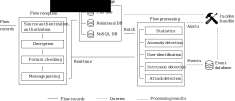
\includegraphics{figures/c02/flow-processing-details}
  \end{center}
  \caption{Flow data processing schema.}
  \label{fig:flow-processing-details}
\end{sidewaysfigure}

\subsection{Flow Collection}\label{subsec:flow-collection}

Flow collection is a process of receiving flow records from an exporter performed by a flow collector. The collector and the exporter must choose an appropriate combination of transport protocol and flow export protocol before the data transmission starts as there is no protocol for flow export parameters negotiation. Although the collector can receive data using multiple combinations of protocols at the same time, such feature is not usually implemented due to added complexity.

After the collector validates that a received message is in the expected format, it attempts to parse individual flow records. This process may vary for each flow export protocol; however, the collector always needs to derive correct data types of information elements in order to be able to work with them. The common practice with NetFlow information elements was to hardcode their definitions and extend the code every time it was necessary to add a new element. The extensibility of the IPFIX protocol information elements through the use of Private Enterprise Numbers advocates more dynamic approach to information element handling, although a subset of IPFIX information elements are sometimes hardcoded as well. Since the collectors cannot know all possible information elements that can be sent by exporters, it is necessary to handle new and unknown elements correctly. Although they are usually discarded, it is also possible to process them when their data types can be derived from the information provided by the flow export protocol.

When using NetFlow and IPFIX protocols in combination with the UDP transport protocol, it is necessary to properly manage templates messages containing the definitions of flow record formats. The templates can change during the collection process, e.g. after exporter restart, and it can easily result in incorrectly decoded messages. The IPFIX protocol specification~\cite{rfc7011} describes how the template messages should be handled and what to do in case of missing templates. Both NetFlow and IPFIX protocols keep track of lost messages by assigning a sequence number to each message. NetFlow~v5 increase the sequence number for each transmitted flow record, which allows keeping track of the number of lost flow records. This behaviour was changed in NetFlow~v9 so that the sequence number is increased for each transmitted NetFlow~v9 packet. It is more difficult to keep track of the number of lost flow records in NetFlow v9, but easy to see how many packets were lost, which can help with determining the cause of the packet loss. The IPFIX protocol increments the sequence number per flow record, just like NetFlow~v5. However, when a template is missing, it is not possible to determine the exact number of flow records in a packet. Therefore the collector cannot be sure whether flow records were lost during the transmission or not. This is one of several reasons to use IPFIX over a reliable channel.

An important and often neglected aspect of flow collection is security. The collector needs to authenticate the source of the data to avoid processing of malicious flow records or malformed messages intended to attack the collector itself. There are several ways to authenticate the source of the data. IP addresses can be used to authenticate the flow exporter and the collector itself, or a firewall can be set to allow data from authorised IP addresses. However, this does not prevent attackers with the ability to spoof IP addresses when UDP transport protocol is used. Moreover, the Man-in-the-middle (MITM) attack cannot be prevented without the appropriate use of cryptography. Proper authentication, usually using certificates, is needed to mitigate the MITM attack. The IPFIX protocol requires TLS version 1.1 to be implemented for TCP and DTLS 1.0 to be implemented for STCP and UDP protocols. Moreover, it requires mutual authentication when using TLS or DTLS so that the exporter does not send sensitive data to an unknown target. Table~\ref{tab:flow.protocols.security} shows how IP spoofing and MITM attack are mitigated by use of TLS and DTLS protocols. The advantage of TLS and DTLS protocols is that they provide not only authentication but also integrity and confidentiality. Since an IP address is often considered to be sensitive information, ensuring confidentiality of flow records during transmission should be considered a necessity.

\begin{table}[t!]
    \centering
    \begin{tabular}{lll}
    \toprule
            & \textbf{IP Spoofing}    & \textbf{Man-in-the-Middle}  \\ \midrule
    UDP        & yes            & yes \\ 
    TCP        & no            & yes \\ 
    SCTP        & no            & yes \\
    DTLS/UDP    & no            & no  \\
    TLS/TCP        & no            & no  \\ 
    DTLS/SCTP    & no            & no  \\ \bottomrule
    \end{tabular}
    \caption{Applicability of IP spoofing and MITM attack to transport protocols}
    \label{tab:flow.protocols.security}
\end{table}

Although the IPFIX protocol requires implementation of TLS and DTLS protocols, not every flow exporter and collector supports it. There are two often used solutions for ensuring the security of flow record transmission. The first is to build a secure channel between exporters and collectors using external tools, such as virtual private networks or stunnel~\cite{Trojnar-2015-Stunnel}. The second solution used in networks that are fully under control of the administrator is to place the exporter and collector in a dedicated network (using private IP addresses) so that they can be accessed only from allowed and trusted address range.


\subsection{Flow Storage}\label{subsec:flow-storage}

There are many uses for flow data~\cite{Li-2013-Review, Umer-2017-Flow}. At first, the data were being used for traffic accounting, and flow records are often kept by telecommunications companies to comply with laws requiring them to store communication records nowadays. Companies and even individuals also keep flow records of their own traffic so that they can investigate breaches and other security issues ex-post. To store the flow data records for a long period of time, the selected data storage format must be space efficient. Another important aspect of flow data storage is its query performance. The requirements for the query performance differ depending on a particular use case. When overall statistics are required, all flow records need to be accessed. In case of a security breach investigation, filters for particular IP addresses and ports are likely to be used so that it is beneficial for the data storage to have some kind of index built on the data.

There are several types of data storage that are used for flow data. Firstly, the data can be stored in a flat file without indexes. This approach is utilised by popular flow data manipulation frameworks SiLK~\cite{Shimeall-2014-Using} and NFDUMP~\cite{Haag-2014-NFDUMP}. The main advantage is that the format is very simple and the data is efficiently encoded. Moreover, both file formats support compression which allows for more disk space to be saved. Flat files also take advantage of the fact that flow data is never updated so the records can be tightly packed.

A second popular approach is to store flow data in a relational database. In case of NetFlow~v5, a single table serves to store all flow records. However, when multiple templates are used for the flow records, such as in NetFlow~v9 and IPFIX protocols, the number of tables grows, and the relational model becomes complicated. Although relational databases are designed to support much more features than needed for flow data (e.g. updates or complex joins), they often lack support for network data types such as IP and MAC addresses. Moreover, their performance and disk space requirements are often worse than that of flat files, as shown by \citeauthor{Hofstede-2010-Network} in~\cite{Hofstede-2010-Network}.

The last approach is to use a NoSQL database to store flow data. Although NoSQL databases do not offer as many features as relational databases, they are meant to be able to handle huge amounts of data. A category of NoSQL databases is columnar databases. Instead of storing each flow record as a single database record, it stores each element of the record in a separate file. The benefit of this approach is that, for example, when a query for a certain IP address is evaluated, only files with IP addresses need to be searched. Other requested elements are read from their own files as necessary after the address is found. This approach reduces the amount of data that needs to be read from the disk; however, it causes more random accesses than when using flat files. More information about comparing flat file approach with a NoSQL columnar database is provided in Chapter~\ref{chap:next-generation-flow}. Document-oriented databases are also a class of NoSQL databases, and their popularity has been increasing lately. Although the performance of most document-oriented databases is not sufficient to handle flow data from large networks, they are used for their flexibility that allows for building prototype analytics applications very quickly. The advantage of document-oriented databases is that the different structure of flow records is of no concern to the database as it considers each entry to be a generic document. Elasticsearch~\cite{Gormley-2015-Elasticsearch} is an excellent example of a such a database.

The list of used approaches is by no means complete. There are many Big Data analytics frameworks, which are being used for flow data storage and analytics, such as Hadoop~\cite{Lee-2012-Toward}. Although it is possible to use almost any data storage for flow data, it is difficult to select the best one, since the criteria differ for each use case. It is for that reason that companies use different flow data storage or develop their own solution in their products.


\subsection{Flow Processing}\label{subsec:flow-processing}

A large amount of information about network traffic and communicating parties can be acquired by a flow record analysis. Many intrusion detection systems use flow records as their primary source of data, especially since deep packet inspection is being made difficult due to the increasing ratio of encrypted traffic. The flow data analysis can be performed either using the stored data or in real time.

When the flow record analysis is performed on stored data, the processing is usually done in batches. The flow collector usually partitions the data according to the time of arrival so that once a partition is finished, it can be processed in a single batch. Five-minute long time windows are often used as this is the default time interval employed by the popular flow processing tool NfSen~\cite{Haag-2011-NfSen}. The advantage of this approach is that the processing can easily be repeated on the same data, which allows the user to fine-tune the queries and analyse the data on demand. The processing can also be postponed when the system is under heavy load. The disadvantage of batch processing with fixed time intervals is that it introduces delays to data analysis, which can be inconvenient when rapid action is required based on the results.

When the delay induced by the batch processing impedes time-critical applications, stream processing can be used instead. In stream processing, the flow records are passed to the processing immediately after they are received. A good overview of the stream-based flow processing is provided by \citeauthor{Jirsik-2017-Toward} in~\cite{Jirsik-2017-Toward}. There is a number of stream processing systems that are used for big data processing. \citeauthor{Cermak-2016-Performance} performed flow data analysis using three most used distributed stream processing systems in~\cite{Cermak-2016-Performance}, and compared their performance. The results show that the distributed stream processing systems are able to scale to accommodate large workloads such as processing of data from very large networks.

The flow processing can be used to achieve several goals. Firstly, both live and long-term network statistics can be computed. Live statistics are used by administrators to gain an overview of a network situation. This is useful for tracking down problems and optimising network configuration when the changes take effect immediately. The long-term statistics provide useful information for capacity planning. Secondly, flows can be used to gain situational awareness about the network and connected devices~\cite{Lastovicka-2017-Situational}. This includes device identification and application classification, which often use machine learning techniques for this purpose. Thirdly, flows are nowadays frequently in intrusion detection systems used to detect attackers on a network, as described by \citeauthor{Umer-2017-Flow} in~\cite{Umer-2017-Flow}. Lastly, anomaly detection techniques are being applied to flow data to detect suspicious behaviour which might indicate a problem or attack on the network. There are many anomaly detection techniques as surveyed by \citeauthor{Chandola-2009-Anomaly} in~\cite{Chandola-2009-Anomaly} and significant effort was put to applying these techniques to flow data by various researchers.

Modern machine learning techniques are utilised in flow processing. The most common uses are in traffic classification~\cite{Velan-2015-Survey}, user identification~\cite{Verde-2014-No} and intrusion detection~\cite{Tsai-2009-Intrusion}. Although the research in this area is quite extensive, the authors of~\cite{Sommer-2010-Outside} show that the results are seldom applied in practice and provide several observations explaining the difficulties faced by the implementers. A survey of traffic classification techniques for encrypted traffic is provided in Chapter~\ref{chap:measurement-of-encrypted-traffic}.


\section{Common Issues}\label{sec:common-issues}

Although flow monitoring is widely used, there are many not widely known aspects that need to be taken into consideration during its deployment. This section describes several issues that can be encountered in any flow monitoring system and that are easily neglected. We draw mainly from our experience of running the flow monitoring infrastructure of CESNET National Research and Education Network in this section. Most issues concern data loss. Either the data is not correctly observed, parsed, are lost during transmission, or are not interpreted correctly. Firstly, we look at the more obvious and readily detectable issue where no data arrive at all. Then we describe the issues that cause data loss which is not easily detected. Lastly, we discuss issues and misunderstandings that cause the data to be incorrectly measured and interpreted. Let us note here, that suitable logging facilities of flow exporter and collector together with a reliable log processing mechanism can help to discover many of the described issues.

\subsection{Visible Data Loss}

The usual cause of data loss is that the monitoring infrastructure is misconfigured. Whether it is due to a misconfiguration at the flow exporter or the flow collector side, the obvious indication of the problem is that no data are stored and no results of the flow data processing, such as statistics, are generated. As the problem is quite easily observed, its cause is easily detected. The best way is to review the whole flow processing setup from packet observation to flow storage and processing to see at which point the data are lost.

The first component to investigate is the packet observation. It is possible that the data are no longer sent to the observation point, possibly due to a failed TAP device or a router misconfiguration. This can be easily confirmed using interface packet counters. Even if the data arrive at the observation point, the flow exporter might be configured to read data from an incorrect interface. When the flow exporter is receiving and processing the data, it is important to audit the flow export settings. The data might be sent to an incorrect destination or using incompatible transport or flow export protocol. When TLS/DTLS is used, the certificates and keys might not match. It is a good practice to verify that the data actually leave the probe, for example by using a tool such as \emph{tcpdump}.

Since the flow probe is often placed in a dedicated network, it is useful to verify that the network is configured to allow the communication between the probe and the flow collector.

The flow collector must be configured to accept data from the flow exporter, which includes a proper setup of certificates and keys. Even when the flow collector receives the data, it might be running using incorrect configuration, and the data might be saved to an unexpected location or not passed to storage and processing at all. A collector may also decide to discard flow records containing unknown information elements. When the flow exporter includes such an element in every record, all flows are dropped. 

\subsection{Unobserved Data Loss}

It is impossible to continuously verify that all observed packets are accounted for in the flow records processed by the flow collector. Since each flow record contains information from packets observed at a different time interval, it is not possible to compute the exact number of packets that passed an observation point from the respective flow data. All statistical information about the number of transferred packets is to a certain level biased. The only test that can be continuously applied is that the total number of observed packets at the observation point and the flow collector remain in a similar range. Since it is not possible to verify that every packet is observed, some packet of even flows might be lost in the flow monitoring process without notice.

There are many networking protocols in use nowadays. Although all flow exporters support the basic protocols such as IPv4, TCP, UDP, and ICMP, they also need to be able to process many data link layer protocols, such as VLAN, VXLAN, MPLS, TRILL, and others. When a new protocol is used on the network for which the flow exporter is not ready, the flow record cannot be created, and the information is lost. A similar issue involves tunnelling protocols, such as GRE or protocol 41. For example, when the original IP packet is encapsulated in another L3 protocol, it is important to decide whether the flow record should be created from the inner or outer L3 header. Without an additional mechanism to provide more information about the tunnelled traffic, information from one of the headers is lost.

Flow records containing unknown informational elements might be discarded by the flow collector, as described in the previous section. However, when only some of the flow records contain such information elements, the issue is harder to observe. Therefore it is necessary to have a good knowledge of the used flow collector and its behaviour.

Sometimes messages can be longer than the MTU of the link between the flow exporter and flow collector, especially when application layer information is contained in the flow records. In such a case, use of UDP transport protocol might cause data loss as fragmented packets are sometimes blocked by firewalls. Moreover, the packet loss is more probable since by losing a single fragment the entire message is unreconstructable and must be discarded. When such a long messages need to be sent, it is best to use a reliable transport protocol such as TCP or SCTP.

One of the most common reasons for data loss in flow monitoring is that the performance of flow exporter or a flow collector is not high enough to process all data. There are several places where either packets or flow records might be dropped, as shown in Figure~\ref{fig:flow-packet-drop}. The first is the source of data for the observation point. When the data to the observation point are provided using router SPAN port, the capacity of the SPAN port must be equal or greater to that of individual links that are measured; otherwise, some packet will be dropped by the router when there is too much traffic. This is not an issue when using a TAP because the TAP always splits a single link or a duplex link to two links of the same type and capacity. The second point where packets are often dropped is the observation point. When the exporter does not process the data before the packet reception buffer is full, the newly arrived or the oldest packets are dropped, based on the implementation of the buffer. The third point where the data might be dropped is on the collector device. When the flow collector does not process data quickly enough, the system packet reception buffers fill up, and new packets are dropped. This is similar to the packet drop on flow probe; however, every packet lost at the collector contains several flow records that were created from many packets. Therefore, loss of packets with complete flow records is much more severe.

\begin{figure}[t!]
  \begin{center}
    
\includegraphics{figures/c02/flow-packet-drop}
  \end{center}
  \caption{Flow monitoring packet drop schema.}
  \label{fig:flow-packet-drop}
\end{figure}

The choice of transport protocol has an impact on the packet drop as well. UDP messages are discarded by the collector when it does not process in a timely manner. However, using a congestion-aware protocol such as TCP and SCTP, the collector might create backpressure on the flow exporter so that it cannot send new messages when it needs to. Therefore, the flow exporter can either drop such messages or wait for the collector to process more data. However, when the flow exporter does not drop the messages, it creates backpressure on the flow cache, packet processing, packet parsing and packet reception. This way the slow processing on collector might easily lead to packet drop at the observation point. Another reason for flow exporter not being able to send messages is a slow link between the exporter and collector. When application information is present in the flow records, the required throughput might easily exceed 100\,Mbps, especially when the exporter sends data to multiple collectors. Although such slow links are not used very often nowadays, they might still be encountered in practice.

Although packet drop should be avoided at both flow exporter and flow collector sides, sometimes it is necessary to drop packets in a controlled manner, e.g. under a DDoS attack. We recommend creating a packet buffer in the application to which the data is always stored. Then, when the data processing is slow, and the buffer becomes full, the application can decide which packets to drop. The advantage of this approach is that the application is aware of the congestion and can adequately react to it, e.g. by reporting it or limiting the processing to a bare minimum.

A frequent cause of packet loss at the collector side is the shutdown or restart of flow exporter. The flow exporter usually expires all flow records in the flow cache so that they are not lost. However, as the flow cache may contain hundreds of thousands of flow records, exporting them all at one at the highest possible rate (the flow exporter needs to shut down or restart without an unnecessary delay) can overwhelm the flow collector. Therefore, it is best to implement two types of shutdown, emergency and graceful. In the emergency shutdown, the data in the flow cache are simply discarded as they are not considered important. This allows to quickly shut down or restart the exporter, which is beneficial during testing and for important configuration changes. The graceful shutdown should have a configurable flow record export rate. This allows to adapt the capabilities of the flow collector without overwhelming it and limiting the risk of data loss.

Flow monitoring performance is discussed in detail in Chapter~\ref{chap:flow-monitoring-performance}.


\subsection{Other Issues}

There are other problems that can be encountered during flow monitoring apart from the performance issues and data loss. We have already described the problem with counting lost flow records and elements in The Subsection~\ref{subsec:flow-collection}. This section describes the most common of the issues that cause the data to be incomplete or incorrect.

The first issue is encountered by flow exporters that process biflows. To process biflows correctly, the exporter needs to observe both directions of each flow. There are several reasons why it may fail to do so. Only single direction might be connected to the probe, or the network configuration might route the packets asymmetrically. Even if both directions can be observed at the observation point, packets might be received, parsed, and processed in several different queues to speed up the monitoring process. In such a case, it is essential to use a correct algorithm to select queues for packets; otherwise, the packets from opposite directions may end up in different flow caches, and the created biflows will be incomplete. The algorithm must be able to work with all packet headers that precede the headers from which the flow keys are derived. 

Both the flow exporter and flow collector must agree on the semantics of the elements of exported flow records. For example, the packet length is usually exported in IPFIX format as a \emph{octetDeltaCount} element. The specification~\cite{IANA-2017-IP} defines it to be the number of octets since the previous report (if any) in incoming packets for this Flow at the Observation Point. The number of octets includes IP header(s) and IP payload. However, some exporters put the total number of octets including the link layer in this field. Moreover, the IPFIX protocol is sometimes used to export information about non-IP flows as well, so that this element is used differently for specification. Whether the exporter and collector adhere to the specification, it is important that they interpret the semantics equally. In this case, it would be proper to set up a different element with different semantics if the total number of octets needs to be reported.

Different exporters can encode flow record elements to integers, strings and byte arrays of different length. For example, the IPFIX protocol supports \emph{Reduced-Size Encoding}~\cite{rfc7011} which allows encoding elements using fewer octets than the number specified by~\cite{IANA-2017-IP}. Although this saves resources such as the memory of the flow exporter, network bandwidth, and disk space on the collector, it makes it more difficult to process correctly. When the same element is received by the collector using two different data types, it needs to decide which is going to be used for further processing as maintaining both original data types is cumbersome. The collector usually converts the data to the largest possible data type since it cannot know in advance whether it will receive the element encoded differently in the future and reducing the size of an element may lead to information loss.

The encoding of TCP flags in IPFIX protocol is a good example of issues that can be caused by the \emph{Reduced-size Encoding}. NetFlow~v9 defined TCP flags element as one byte, and the IPFIX used single byte as well originally. However, the TCP control bits occupy nine bites in the TCP header~\cite{rfc3540}; therefore, a change was proposed in 2013 to change the encoding to two bytes. The discussion resulted in RFC 7125~\cite{rfc7125} in 2014 with IPFIX supporting the export of TCP flags as a two-byte value, as shown in Figure~\ref{fig:tcp-flags}. When reduced size encoding is used, only the original byte is exported for backwards compatibility. This presents the authors of flow collectors with a difficult issue. If they support TCP flags as a two-byte value, they must indicate that the received element was only a single byte long. Storing the two-byte value and padding with zeroes is not an option since that would set the ECN nonce sum flag to zero although the collector has no knowledge of its original value.

\begin{figure}
  \begin{center}
    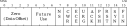
\includegraphics{figures/c02/tcp-flags}
  \end{center}
  \caption{TCP control bits export in IPFIX protocol~\cite{rfc7125}.}
  \label{fig:tcp-flags}
\end{figure}


\section{Summary}\label{sec:nfm-summary}

This chapter has explained flow monitoring, its history, common uses, and discussed related technologies that are sometimes confused with flow monitoring. We have shown, that the currently used definitions of a flow do not reflect the reality of real-world flow monitoring deployment. Therefore, we have provided an improved definition that amends the deficiencies. We have also created a formal notation for our definition which allows us to avoid misunderstandings created by the use of informal language. It also allows flow related algorithms to be written more precisely and concisely.

The rest of the chapter has discussed details of the flow monitoring process from the packet capture on a probe to the flow processing on a collector. We have also shown the most common issues that can be encountered while deploying and operating a flow monitoring infrastructure. The most critical issues are caused by incorrect implementation and low performance. We investigate the performance of flow monitoring in Chapter~\ref{chap:flow-monitoring-performance}.


\chapter{Application Flow Monitoring}

\begin{chapintro}

Deep packet inspection (DPI) and IP flow monitoring are frequently used network monitoring approaches nowadays. Although the DPI provides application visibility, detailed examination of every packet is computationally intensive. The IP flow monitoring achieves high performance by processing only packet headers, but provides less details about the traffic itself. Application flow monitoring is proposed as an attempt to combine DPI accuracy and IP flow monitoring performance. This chapter ... 
% contributions

% Petr Velan and Pavel Čeleda. “Next Generation Application-Aware Flow Monitoring” - related but cannot be directly included.
% Petr Velan, Tomáš Jirsík, and Pavel Čeleda. “Design and Evaluation of HTTP Protocol Parsers for IPFIX Measurement”
The papers related to this chapter are~\cite{Velan-2014-Next, Velan-2013-Design}.

The organisation of this chapter is as follows:
\begin{itemize}
  \item Section~\ref{sec:creating-application-flow} 
  \item Section~\ref{sec:http-parser-design}
  \item Section~\ref{sec:app-conclusions} concludes the chapter.
\end{itemize}

\end{chapintro}

\newpage


\section{Motivation}
The number of different applications communicating over the Internet is ever increasing and so is the need for application-aware network monitoring. However, building network monitoring systems is always a compromise between accuracy and performance. The more information processed, the more accurate the monitoring system is. Unfortunately, thorough examination of the traffic is computationally expensive~\cite{Gao-2006-Efficient, Lai-2004-Parallel}. Application flow monitoring is a network monitoring approach created to exploit the benefits of deep packet inspection (DPI). Integration of the DPI into flow monitoring allows for information aggregation, which provides better performance than the DPI alone.

Application flow monitoring is a subset of flow monitoring as described in the Chapter~\ref{chap:network-flow-monitoring} and all provided definitions hold for it as well. The reason to treat application flow monitoring as a special case is that processing application layer introduces specific issues and requires special attention. Therefore, we distinguish IP flow monitoring (flow keys and values of other properties  are extracted only from link, network, and transport layer headers) and application flow monitoring as two distinct part of flow monitoring.

The application flow monitoring usually utilizes two main concepts: application identification (also known as traffic classification) and application visibility. The application identification allows to recognize the application protocol of a particular flow. The type of application is usually added as a single field to the exported flow record. The application visibility provides more information about the information carried by the application protocol itself. Application identification is a prerequisite of the application visibility. However, application identification can be done with use of machine learning techniques even without observing packet payloads.

This chapter describes the differences between IP flow monitoring and application flow monitoring that have to be taken into consideration when the application flow monitoring process is designed and deployed. The most important part of application visibility is the design of application parsers. To illustrate the complexity of the application parser design, we propose and discuss several designs of HTTP protocol parsers at the end of this chapter.

The benefits of application flow monitoring are discussed extensively in the Chapter~\ref{chap:traffic-analysis-using-application-flow-monitoring}.

\section{Related Work}

The use of machine learning techniques for traffic classification has attracted many researchers~\cite{Nguyen-2008-Survey, Dainotti-2012-Issues, Finsterbusch-2014-Survey}. A complete survey of the used techniques and results is out of scope of this work, however, the methods of application identification for encrypted traffic is surveyed in the Chapter~\ref{chap:measurement-of-encrypted-traffic}.

Although application visibility is provided by a variety of commercial products such as dedicated probes, forwarding devices, and firewalls, it does not seem to be as attractive research topic as application identification. However, significant research effort was invested in automating the creation of application parsers. \citeauthor{Pang-2006-binpac} created a language and accompanying parser called \emph{binpac}~\cite{Pang-2006-binpac} in \citeyear{Pang-2006-binpac}. It allows to generate application parsers from their declarative description. A slightly different approach was taken by \citeauthor{Caballero-2007-Polyglot} in \citeyear{Caballero-2007-Polyglot}. The authors created a tool called \emph{Polygot}~\cite{Caballero-2007-Polyglot} which is used to reverse engineer application protocol headers. Similar work was published at the same time by \citeauthor{Cui-2007-Discoverer} in \cite{Cui-2007-Discoverer}. They presented a tool called \emph{Discoverer} that could automatically reverse engineering the protocol message formats of an application from its network trace. \citeauthor{Davidson-2009-Protocol} introduce a notion of using a higher order attribute grammar in~\cite{Davidson-2009-Protocol}, which allows to describe the structure of application protocols for which the use of context-free grammar is impractical of impossible. Another framework, called \emph{Spicy}~\cite{Sommer-2016-Spicy} was introduced by \citeauthor{Sommer-2016-Spicy}. It consists of format specification language, compiler toolchain and an API for DPI applications which allows for easy integration of the generated parsers to existing tools.

% say that the IFPIX allows addition of new application elements and that the NetFlow was very limiting.

% opensource: nProbe, yafdpi
% commercial: Cisco (appliance and firewall), FlowMon (https://www.flowmon.com/en/products/flowmon/probe), Lancope (https://www.lancope.com/products/stealthwatch-flowsensor), ntop, some firewalls (barracuda networks (https://www.barracuda.com/products/nextgenfirewall_x/features), dell, aerohive networks, palo alto networks (https://www.paloaltonetworks.com/features/application-visibility))

\itodo{
- Cisco Application Visibility and Control\\
- \url{http://www.cisco.com/c/en/us/products/routers/avc-control.html}\\
}

\itodo{
- Network-Based Application Recognition (NBAR)\\
- \url{https://www.cisco.com/c/en/us/products/collateral/ios-nx-os-software/network-based-application-recognition-nbar/prod\_case\_study09186a00800ad0ca.html} \\
- NBAR2 \\
- \url{https://www.cisco.com/c/en/us/products/collateral/ios-nx-os-software/network-based-application-recognition-nbar/product\_bulletin\_c25-627831.html}
}

\itodo{lucaderi ntop\\
\url{http://www.ntop.org/nprobe/unveiling-application-visibility-in-ntop-and-nprobe-both-in-netflow-v9-and-ipfix/}}

\itodo{yaf \cite{Inacio-2010-YAF}\\
\url{https://tools.netsa.cert.org/yaf/yafdpi.html}\\
\url{https://tools.netsa.cert.org/yaf/applabel.html}}

\section{Application Flow Definition}
% application flow is a subset of flow as defined in chap 2.
% application flow definition (in text) 
% beware of application identification vs application visibility, it must fit the definition

% explain that aplication flow monitoring means that:
% - primary: information from application layer is added to flow records
% - secondary:
%  - application logic (not necessarily in L7) affect the flow creation process, e.g. monitoring of tunnels
%  - less typical but can also be considered as application flow monitoring: additional information can be added to flow records from external sources (geolocation)

\section{Creating Application Flow}\label{sec:creating-application-flow}
% 
% application flow monitoring changes to flow monitoring (sometimes called IP flow monitoring):
% - packet processing: 
%   - L7 parsing is sometimes complex -> section with Design of an HTTP Parser
%   - need to support recursion for tunnel monitoring
% - flow creation
%   - more complex flow keys
%   - split flows after application event (next request in a single connection (HTTP pipelining))
%   - retain application data for flows split by active timeout
%   - size of flow records -> large flow caches
% - flow export
%   - described in previous chapter - long flows, different semantics for new elements
%   - when URLs, domain names etc are exported in fixed lenght, the original length should be exported as well



\iinfo{Taken from: Application Flow Monitoring Challenges}

\itodo{TODO: vyporadat se s opakujicimi se hlavickami (HTTP), doplnit definici flow z predchozi kapitoly\\
- Flow expiration/termination vs app flow splitting}

The application flow monitoring is a complex process. Packets need to be received from the network, transported to computer memory (RAM), parsed, aggregated to flow records based on the parsed information, and exported to flow collectors for further processing. The process is depicted in Figure~\ref{fig:flow-exporter-schema}. This section describes the whole flow measurement process, points out where it is affected by the application processing and introduces some of the related challenges.

\begin{figure}[tb!]
  \begin{center}
    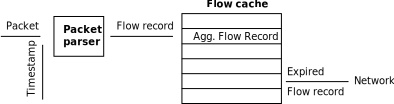
\includegraphics[width=\textwidth]{figures/flow-exporter-schema}
  \end{center}
  \caption{A Flow Exporter Schema}
  \label{fig:flow-exporter-schema}
\end{figure}


The packet reception is unchanged for application flow monitoring unless the NIC processes the application layer. This scenario is discussed later in Hardware Accelerated Techniques section.


\subsection{Packet Processing}

% \cite{Pang-2006-binpac}

The basic task of the packet parsing is to extract connection attributes such as IP addresses, transport protocol, and ports to determine which flow the packet belongs to. Moreover, it obtains additional information of interest, especially from application protocols. The parser must be resilient to malformed packets and unknown protocols while supporting a wide range of existing network and application protocols.

Link, network, and transport headers of IP packets follow a strictly defined structure so that the network devices such as routers can process the packets swiftly. However, application layer protocols often rely on connections being established between compatible endpoints. For this reason, application protocol identification is a difficult task. A lot of attention has been dedicated to research of application identification in network traffic in the past, for example in the work of \citeauthor{Bujlow-2015-classification}~\cite{Bujlow-2015-classification}, however, not every approach is suitable for the flow monitoring scenario.

With increasing deployment of encryption for all kinds of communication, the task of application flow monitoring becomes more difficult. Without access to application payload, the amount of information that can be extracted from the traffic is diminished. However, there are statistical and machine learning methods that are able to recognize specific applications even in encrypted traffic with high accuracy. Moreover, useful information such as a version of encryption protocol, certificates, or supported cipher suites, can be extracted from encrypted traffic. This information can be used to identify malicious encrypted traffic. The possibilities of processing and analysis of encrypted traffic were surveyed by the authors of~\cite{Velan-2015-Survey}.

\subsection{Flow Creation}

Application protocol measurement may require flow record to be expired early. For example, when HTTP protocol supports pipelining, multiple requests and responses can be carried out over a single connection. When it is desirable to keep track of each request/response pair, existing flow record might be exported when a new request is encountered on the same connection. Therefore, application flow monitoring  also affects the number of generated flow records, which needs to be taken into consideration during further processing of the flow records.

\iimprove{TODO: keeping application data from expired flow records (long HTTP video streaming)}

Another impact of the application flow monitoring on the flow aggregation is the increased size of flow records. The information extracted from application protocols can be quite large in comparison to network and transport layers lengths. While the typical IPv4 header length is 20 bytes, typical TCP header length is 32 bytes, the HTTP URL can easily be several hundred bytes long. Therefore, the length of flow records of application flow monitoring is several times larger than without the application layer. There are two main negative impacts of such large flow records. Firstly, the flow cache might require much more RAM than standard flow monitoring flow cache. Secondly, even if the cache fits into RAM, it degrades the performance of the memory accesses because data locality is decreased and a CPU experiences more cache misses. For these reasons, it must be carefully considered which information is placed in each flow record and how it is encoded.

\subsection{Flow Export}

Several issues might be encountered with flow export when application flow monitoring is applied. First, due to the larger amount of exported data, the link to a flow collector might be congested. We have experienced this issue when application flow records from a 10G link were exported simultaneously to several collectors over old 100\,Mb/s management interface. The solution is either to simply upgrade to 1\,Gb/s management interface or, better, to reduce the number of targets of the export and distribute the flows as necessary through replicating proxy in the location of the collectors. The latter solution saves network bandwidth used for monitoring purposes and should be preferred if possible.

Another issue that might be encountered due to large flow record is that single record might be larger than MTU of the management network interface on the flow exporting device. In such a case UDP transport protocol, which is still widely used for flow export, cannot be used without fragmenting IP packets. The fragmentation might cause a performance problem for the flow collector which has to reassemble the packets. It also increases the probability of data loss as single lost fragment invalidates the whole message.


\section{Common Issues} % what is specific to application protocols, otherwise it should be at the end of previous chapter

% shortening of string values - add some indication of shortening or original length

\section{Design of an HTTP Parser: A Study}\label{sec:http-parser-design} % put in Velan-2013-Design paper 

\section{Conclusions}\label{sec:app-conclusions}

\chapter{Traffic analysis using Application Flow Monitoring}\label{chap:traffic-analysis-using-application-flow-monitoring}

\begin{chapintro}

There are many usages for application traffic monitoring. The common goal is to extend the set of collected information elements and thus provide a deeper understanding of network traffic. This chapter shows several use cases for application flow monitoring, which were published in separate papers. The contribution of this chapter is a summary of the contributions of those papers.

As a first example of traffic analysis with the use of application flow monitoring, we show how information from HTTP headers can be used to detect new classes of attacks on the application layer. This is the most common use case for application flow monitoring. 

% Basic flow monitoring usually stops after the first header following the IP layer. However, the IPv6 protocol allows header chains of an arbitrary length. Therefore, we have extended the analysis of IPv6 protocol, so that information about multiple chained headers is collected for each flow. An analysis of chained headers is performed, and we attempted to interpret their usage. Moreover, we show that these chained headers can be used for attacks and also show, how to detect such attacks using the application flow monitoring. In addition to this work, we also show how IPv6 transition mechanisms can be monitored so that even tunnelled IPv6 traffic can be monitored.

Basic flow monitoring usually stops after the first header following the IP layer. However, many networks and networking protocols utilise encapsulation to traverse over network segments with unsupported equipment or to allow aggregating of traffic into virtual networks. IPv6 transition mechanisms are a distinctive class of protocols used to provide IPv6 connectivity over IPv4 networks. Most operating systems provide means to deliver IPv6 connectivity even when native IPv6 is not available. Therefore, we extended the basic flow monitoring with information from the IPv6 transition mechanisms and we report on the IPv6 deployment and the use of the transition mechanisms.

Inserting information to the flow records from external sources is also considered to be a variant of application flow monitoring. We show an example of adding geolocation information both in the flow exporter and collector. We show that both implementations scale very well and that the geolocation data can be used for advanced traffic analysis.

Since most flow monitoring experiments are performed on a live network, it is impossible to replicate the results exactly. We show a method of characterising network traffic so that it is possible to compare multiple network traces and search for similarities. This allows us not only to compare different networks but to quantify changes in network profile in time.

% Martin Husák, Petr Velan, and Jan Vykopal. “Security Monitoring of HTTP Traffic Using Extended Flows”.
% Martin Elich, Petr Velan, Tomáš Jirsík, and Pavel Čeleda. “An Investigation Into Teredo and 6to4 Transition Mechanisms: Traffic Analysis”.
% Pavel Čeleda, Petr Velan, Martin Rábek, Rick Hofstede, and Aiko Pras. “Large-Scale Geolocation for NetFlow”
% Luuk Hendriks, Petr Velan, Ricardo de O. Schmidt, Pieter-Tjerk de Boer, and Aiko Pras. “Threats and Surprises Behind IPv6 Extension Headers”.
% Luuk Hendriks, Petr Velan, Ricardo de O. Schmidt, Pieter-Tjerk de Boer, and Aiko Pras. “Flow-Based Detection of IPv6-specific Network Layer Attacks”
% Petr Velan, Jana Medková, Tomáš Jirsík, and P. Čeleda. “Network Traffic Characterisation Using Flow-Based Statistics”. - needs proper intro in chapintro, or move to next chapter
The papers included in this chapter are~\cite{Husak-2015-Security, Elich-2013-Investigation, Celeda-2013-Large, Velan-2016-Network}. Other papers related to this chapter are~\cite{Hendriks-2017-Flow, Hendriks-2017-Threats}.

The organisation of this chapter is as follows:
\begin{itemize}
  \item Section~\ref{sec:analysis-http-flows} analyses HTTP traffic in a large-scale environment with the use of application flow monitoring. The added value of application flow monitoring is established by detection of several previously undetected attacks.
  \item Section~\ref{sec:analysis-ipv6-transition} reports on IPv6 deployment and the use of transition mechanisms. The basic flow monitoring is extended by the capability of analysing a tunnelled IPv6 traffic.
  \item Section~\ref{sec:analysis-geolocation} shows how flow records can be extended with geolocation information and how this additional information can be employed for network analysis.
  \item Section~\ref{sec:analysis-characterisation} proposes a network traffic characterisation method using flow-based statistics. The characteristics are used to understand and describe the nature of the traffic better and to compare different network traces against each other.
  \item Section~\ref{sec:use-cases-summary} summarizes the chapter.
\end{itemize}

\end{chapintro}

\newpage

\section{Security Monitoring of HTTP Traffic Using Extended Flows}\label{sec:analysis-http-flows}

HTTP is currently the most widely used protocol which takes up a significant portion of network traffic. Due to its popularity, it is beneficial to have a deeper understanding of HTTP network traffic and its content. From a network security perspective, we would like to know who is accessing our network and what the requested resources are. Patterns in network traffic and outstanding numbers of visited hosts and requested resources would help us to distinguish between legitimate and malicious traffic. The most suitable way of gaining an overview of HTTP traffic in a large-scale network is application flow monitoring, as defined in the previous chapter.

We address two problems in this section. The first one is the lack of an overview of network traffic and insufficient security awareness. This applies especially in heterogeneous networks with distributed administration. Many administrators oversee web servers in their administration and may oversee their neighbourhood, but they are not aware of security threats in the rest of the network. The second problem is to find a suitable set of tools to analyse HTTP traffic and distinguish between legitimate and malicious traffic.

To formalize the scope of our work, we pose two research questions which we shall answer:
\begin{itemize}
\item[\emph{(i)}] \emph{What classes of HTTP traffic relevant to security can be observed at network level and what is their impact on attack detection?}
\item[\emph{(ii)}] \emph{What is the added value of application flow monitoring compared to basic flow monitoring from a security point of view?}
\end{itemize}

The first question is focused on common types of HTTP traffic that we can observe in the network. We expect to extend the traditional division of network hosts into clients and servers. We focus on the behaviour of hosts regardless of their client/server role: we are particularly interested in detecting security-related patterns produced by attackers, proxies, and crawlers. We search for implications of the presence of particular traffic patterns. We aim to improve malicious traffic detection, filter out false positives, apply better security policy, and set up trustworthy honeypots.

The second question is focused on evaluating the contribution of application flow monitoring with respect to the detection of malicious behaviour in the network. We focus on the detection of patterns in the network traffic that are hard to observe using basic flow. Application flow would make detecting these events straightforward.

Our work contributes to a better understanding of current security threats. For example, we can detect vulnerability scanners and learn about vulnerability itself at the same time.

The answers to both questions are based on an analysis of real traffic in a campus network. We use network application flow monitoring processing the information from HTTP application layer, which provides HTTP elements to application flow records. Although it is possible to extract some information, such as the Server Name Indication, from the HTTPS protocol, this work focuses on the HTTP protocol only.

We also use auxiliary methods to verify and validate the results, i.e., to confirm the membership of detected IP addresses into the proposed behaviour classes. Legitimate sources of traffic should be identifiable, e.g., Googlebot can be identified by a reverse DNS record of the source IP address~\cite{Google--Verifying}. We check User-Agents in HTTP traffic to differentiate legitimate and illegitimate traffic, e.g., requests with forged User-Agent. Finally, we check the reachability of traffic destination through search engines to see if it is possible to find the resource without accessing it. We follow the principle of ``Google Hacking''~\cite{Billig-2008-Evaluation}, a technique used for finding vulnerabilities on web pages indexed by search engines.

This section is divided into six subsections. Subsection \ref{subsec:httpsecurity-related_work} presents previous work in this field. Measurement tools and environment are described in Subsection \ref{subsec:httpsecurity-measurement}. The results are presented in Subsection \ref{subsec:httpsecurity-results} and discussed in Subsection \ref{subsec:httpsecurity-discussion}. Finally, Subsection \ref{subsec:httpsecurity-conclusion} concludes the section.

\subsection{Related work}\label{subsec:httpsecurity-related_work}

Although research has focused on analysis of HTTP traffic in recent years, there is only a small number of papers relevant to our work. To the best of our knowledge, we are not aware of any paper dealing with HTTP analysis using a flow-based approach. In addition to this, the motivation of the relevant papers is different, typically focusing on efficient traffic management, with only a minor focus on security, specifically attack detection and prevention. One exception is the work by~\citeauthor{Perdisci-2010-Behavioral}~\cite{Perdisci-2010-Behavioral}. They employed network-level behavioural clustering of HTTP requests generated by malware. Their motivation was to provide quality input for algorithms that automatically generate network signatures. The second exception is the work by~\citeauthor{Husak-2014-PhiGARo}~\cite{Husak-2014-PhiGARo} in which they use flow-based HTTP analysis to detect users who contacted malicious websites.

Other related papers dealing with HTTP traffic analysis are listed in this paragraph. \citeauthor{Augustin-2011-Traffic}~\cite{Augustin-2011-Traffic} published a classification of web applications according to three traffic features: intensity (total volume of exchanged traffic), symmetry (ratio between upstream and downstream traffic) and shape (burstiness over time). \citeauthor{Xie-2013-ReSurf}~\cite{Xie-2013-ReSurf} addressed reconstructing web surfing behaviour from network packet traces. \citeauthor{Xu-2014-Toward}~\cite{Xu-2014-Toward} analysed User-Agents strings captured at the edge of a campus network using an extension of UASparser~\cite{Mallat-2017-UASparser}. They identified operating systems, types of devices (mobile, desktop) and applications (browser, crawler, P2P, automated updates and requests). A similar work by~\citeauthor{Jin-2012-Integrated}~\cite{Jin-2012-Integrated} is motivated by efficient traffic management. \citeauthor{Hur-2012-Towards}~\cite{Hur-2012-Towards} proposed a smart phone traffic classification based on grouping User-Agent fields and extracting common strings.

\subsection{Measurement tools and environment}\label{subsec:httpsecurity-measurement}

This section describes the methods and tools used for acquiring the data from our campus network. We shall also provide characteristics of the network, in terms of its size and utilization.

We performed all measurements on the campus network of Masaryk University. The network has more than 40,000 users and 15,000 active IP addresses each day in /16 network segment. The network contains both servers and client stations, including proxy servers and a segment of honeypots. Any incoming traffic to the honeypots is by nature suspicious~\cite{Provos-2007-Virtual}, which helps us to recognize malicious network traffic, e.g., HTTP requests on a honeypot web server. Only moderate filtering rules are applied globally to preserve the network neutrality of the academic environment.

Our primary source of data for network traffic analysis are FlowMon~\cite{FlowmonNetworks--Flowmon} probes located throughout the campus network. These probes use NetFlow and IPFIX protocols to export measured traffic as flow records to central collectors~\cite{Hofstede-2014-Flow}. The collected flows are processed by various anomaly and intrusion detection systems, which report incidents to our CSIRT team. This network-centric approach allows us to monitor a complex network with many servers and services managed by different entities as opposed to host-based approaches such as log analysis. In such a case, it would be very difficult to even obtain system logs from every web server in such a varied environment. The monitored links are mostly 1\,Gb/s and 10\,Gb/s which makes the use of DPI systems impractical, or even impossible in the case of 10\,Gb/s links, due to high processing requirements.

To capture data for this section, we used a probe measuring traffic from a 10\,Gb/s link which connects the campus to the ISP. We deployed measurement of the HTTP traffic on this probe using an application flow exporter. The exporter software supports the extraction of basic elements from HTTP headers, such as host name, document URL (split into hostname and path), User-Agent string, and response code. These elements are then exported using the IPFIX protocol as enterprise elements~\cite{rfc7011}. We used an IPFIXcol~\cite{Velan-2012-Flow} flow collector to receive and store the application flow records.

A basic flow record usually consists of flow keys~\eqref{eq:httpsecurity-flow-key} and of other properties providing detailed information about the flow~\eqref{eq:httpsecurity-flow-additional}. The most common flow keys are L3/L4 protocol numbers, IP addresses, and ports. Additional elements usually contains information from packet headers together with statistical counters, e.g., timestamps, number of packets and bytes, and autonomous system numbers.

\begin{equation} \label{eq:httpsecurity-flow-key}
    \begin{split}
        F_{key} =\ &(L3Proto, srcIP, dstIP, \\
        & L4Proto, srcPort, dstPort)
    \end{split}
\end{equation}

\begin{equation} \label{eq:httpsecurity-flow-additional}
    \begin{split}
        F_{additional} =\ &(timeStart, timeEnd, packets, octets, \\
        & TCPflags, ToS, srcAS, dstAS )
    \end{split}
\end{equation}

A basic flow record is then a concatenation of $F_{key}$ and $F_{additional}$. The HTTP measurement, described in~\cite{Velan-2013-Design}, adds information from the HTTP application layer~\eqref{eq:httpsecurity-key-http}. 

\begin{equation} \label{eq:httpsecurity-key-http}
    \begin{split}
        F_{HTTP} =\ &(hostname, path, userAgent, requestMethod, \\
        & responseCode, referrer, contentType )
    \end{split}
\end{equation}

By concatenating a basic flow record with additional application elements an application flow record is created. In this case, it contains HTTP elements~\eqref{eq:httpsecurity-app-flow}.

\begin{equation} \label{eq:httpsecurity-app-flow}
        F_{app} = F_{key} \cdot F_{additional} \cdot F_{HTTP}
\end{equation}

We measured the $F_{app}$ vector in the environment of our campus network for three weeks over the summer break and three weeks in the semester. Thus, we could compare the amount of overall network traffic and suspicious events over two distinct time periods and traffic loads of the network. The amount of the traffic is lower in the summer break, although still comparable to the rest of the year. However, we assume that the amount of malicious traffic is constant over the year and is more apparent in the summer break.

Table~\ref{tab:httpsecurity-data-sets} shows the size of each dataset in packets, bytes, and flows. Moreover, it contains the number of HTTP requests observed. Although the number of requests is not high compared to the number of flows, there are at least as many responses, which often carry multimedia content. Therefore, the portion of HTTP traffic in bytes is very significant, despite the lower number of requests.

\begin{table}[ht]
\centering
\begin{tabular}{| c | c | c | c | c |} \hline
Dataset &  Flows & Packets & Bytes & HTTP Req.\\ \hline
Summer 2014 & 3.733\,G & 188.953\,G & 198.362\,TB & 0.310\,G \\ \hline
Spring 2015 & 6.680\,G & 552.523\,G & 604.704\,TB & 0.720\,G \\ \hline
\end{tabular}
\caption{Datasets.}
\label{tab:httpsecurity-data-sets}
\end{table}


\subsection{Results}\label{subsec:httpsecurity-results}

Four characteristics of network flows were monitored: source IP address, destination IP address, hostname, and HTTP request. We analysed only HTTP traffic incoming to our network. The destination IP addresses were restricted to the /16 IP range of Masaryk University, while the source IP addresses were restricted to all other IP ranges. In some selected cases, we evaluated also the HTTP requests in opposite direction, i.e., source IP was in our network range and the destination IP was not. We used the hostnames and destination IP addresses interchangeably during the analysis due to a negligible amount of multi-hosting in our network. Overall, we observed HTTP traffic sent to almost 500 web servers, i.e., approximately 3\,\% of all hosts in our network. IPv6 traffic and measurement artifacts were observed in the measurement, but were omitted from the analysis due to their negligible impact on results.

The network traffic was analysed over five-minute and one-day intervals. A five-minute interval is the default granularity of data capture in network flow monitoring, i.e., one output file contains records of five minutes of network traffic. It allowed us to observe local anomalies, not only anomalies in the overall sample traffic. The one-day interval allowed us to compare anomalies over different days and discover repeated events and typical patterns. The one-day time window was chosen as it is long enough to contain an anomaly, while it is short enough in respect to the processing time of an analysis. The statistics presented in this section are based on an analysis of one-day intervals. However, for practical reasons, the five-minute interval is more convenient for detecting malicious events. We checked that the observed events can be detected even in the shorter time window.

We classified the network traffic according to the three main parameters of an application flow record: guest (source IP address), host (destination IP address or hostname), and HTTP request. We were interested in the cardinality of the relation between the parameters rather than values of the parameters. A high occurrence of flows sharing one or more parameters would suggest unusual activity in the network and is key for the classification. The number of flows which share the three main parameters is, therefore, an additional parameter for classification. The parameters and selected classes are presented in Table~\ref{tab:httpsecurity-classes}.

\begin{table}[ht]
\centering
\begin{tabular}{| c | c | c | c | c |} \hline
 &\#Guests & \#Host & \#HTTP Requests & \#Flows \\ \hline
Class I   & 1 &              1 & 1 & n \\ \hline
Class II  & 1 &              n & 1 & n \\ \hline
Class III & 1 & \textgreater 1 & n & \textgreater n \\ \hline
\end{tabular}
\caption{Traffic Classes.}
\label{tab:httpsecurity-classes}
\end{table}

\begin{figure}
  \centering
  \includegraphics[width=0.8\textwidth]{figures/paper-httpsecurity/classes}
  \caption{Selected Classes of HTTP Traffic.}
  \label{fig:httpsecurity-classes}
\end{figure}


We were particularly interested in the results of three queries. First, how many similar requests were demanded by one source IP to one destination IP? Second, how many destination IP addresses were contacted by one source IP address with the same request? And third, how many requests were demanded by one source IP to one destination IP? Each query is represented by a class, as shown in Table~\ref{tab:httpsecurity-classes}. The classes correspond to patterns in the network traffic as depicted in Figure~\ref{fig:httpsecurity-classes}. A detailed description of each query and class can be found in the following subsections.

There are many other possible classes, although we found them to not be relevant from a security perspective. For example, many guests accessing a single host with a request suggests the popularity of a resource at the host. Such classes, however, could be interesting for general traffic classification, not security analysis.

\subsubsection{Class I: Repeated requests}

The first query asks for repeated requests between one guest and one host. We measured the number of occurrences of each triple, consisting of source IP, destination IP, and requested URL. Our assumption was that the repetition itself is common, but outstanding numbers may point to undesired behaviour. For example, password-protected web services may be exposed to brute-force attacks, which we can observe as a series of similar requests. The repeated request (A) is defined as follows:
\begin{equation*}
\begin{split}
Repeated&Request(A) \iff A = \{F \mid \forall F, F':\\
&F(srcip) = F'(srcip) \: \land \: F(dstip) = F'(dstip)\\
&\land \: F(path) = F'(path)\} \: \mbox{ and } |A| > threshold
\end{split}
\end{equation*}
All flows in the set share the same source IP address, destination IP address, and requested HTTP path. The total number of flows in the set is bigger than the threshold.

Sample results are presented in Table~\ref{tab:httpsecurity-repeat} from one day in summer 2014. As we can see, the numbers of repeated flows reaches tens of thousands, which represents outstanding traffic patterns. There is a disproportion in the numbers of flows with the same source IP, destination IP, and HTTP request. While the majority of the triples were unique or repeated several times, a small number of triples were observed to be repeated several thousand times or more. The nature of these repeated requests was revealed by analysing the request. The majority of repeated requests contained a substring such as \textit{admin} or \textit{login}, which suggests that these traffic patterns were caused by brute-force attacks against password-protected web services. Other interesting repeated requests contained the substring \textit{proxy}, which suggests communication between a client and a web-based proxy server. Furthermore, we found other repeated requests accessed large downloadable files, e.g., ISO images of Linux distributions.

\begin{table}[ht]
\centering
\begin{tabular}{| c | c | l | r|} \hline
Guest & Host & HTTP Path & \#Flows \\ \hline
G1  & H1 &                 /wp-\textbf{login}.php & 46,031 \\ \hline
G2  & H2 &      /\textbf{admin}istrator/index.php & 27,965 \\ \hline
G3  & H2 &      /\textbf{admin}istrator/index.php & 27,798 \\ \hline
G4  & H3 &                 /wp-\textbf{login}.php & 25,316 \\ \hline
G5  & H4 & \parbox[t]{5cm}{/pub/linux/slax/Slax-7.x/7.0.8/slax-Chinese-Simplified-7.0.8-i486.iso} & 5,921 \\ \hline
G6  & H5 &           /\textbf{proxy}/lib\textbf{proxy}.pac & 5,036 \\ \hline
G7  & H6 &                        /node/ & 4,286 \\ \hline
G8  & H4 & \parbox[t]{5cm}{/pub/linux/slax/Slax-7.x/7.0.8/slax-English-US-7.0.8-i486.zip} & 4,170 \\ \hline
G9  & H7 &                 /wp-\textbf{login}.php & 3,632 \\ \hline
G10 & H7 &           /polit/wp-\textbf{login}.php & 3,632 \\ \hline
\end{tabular}
\caption{Top Repeated Requests from One Day (Dataset Summer 2014).}
\label{tab:httpsecurity-repeat}
\end{table}

The second sample of results presented in Table~\ref{tab:httpsecurity-repeat2} was observed in one day in spring 2015. As we can see, there is a significant difference in the number of flows. However, the distribution of various types of repeated request is similar. One interesting anomaly is the guest G3, which performed repeated requests on 8 different hosts. This guest used different requests on different hosts, however the number of flows on each host is similar.

\begin{table}[ht]
\centering
\begin{tabular}{| c | c | l | r|} \hline
Guest & Host & HTTP Path & \#Flows \\ \hline
G1  & H1 & /\textbf{proxy}/lib\textbf{proxy}.pac & 5,147 \\ \hline
G2  & H2 & \parbox[t]{6cm}{/pub/linux/fedora/epel/6/x86\_64/ repodata/e63d28ff5a765b11a7052496\\f481f31aebab17c28545908d54e65904a\\1046ec8-filelists.sqlite.bz2} & 4,244 \\ \hline
G3  & H3 & /senat/studenti/wp-\textbf{login}.php & 3,992 \\ \hline
G3  & H4 & /\textbf{admin}istrator/index.php & 3,945 \\ \hline
G3  & H5 & /slovnik/\textbf{admin}istrator/index.php & 3,934 \\ \hline
G3  & H6 & /\textbf{admin}istrator/index.php & 3,926 \\ \hline
G3  & H7 & /capv2011/\textbf{admin}istrator/index.php & 3,924 \\ \hline
G3  & H8 & /index.php & 3,921 \\ \hline
G3  & H9 & /\textbf{admin}istrator/index.php & 3,794 \\ \hline
G3  & H10 & /wp-\textbf{login}.php & 3,701 \\ \hline
\end{tabular}
\caption{Top Repeated Requests from One Day (Dataset Spring 2015).}
\label{tab:httpsecurity-repeat2}
\end{table}

As we can see in Table~\ref{tab:httpsecurity-repeat-statistics}, which displays statistics for the whole monitored time window, almost half of the detected events were related to using a proxy. Brute-force password attacks were recognized only in 10.6\,\% of events. On the other hand, brute-force password attacks may generate more flows than other events in this class. They were the only events which generated more than 10,000 flows with the same source IP, destination IP, and HTTP path. However, we have also observed brute-force attacks of approximately a few thousand flows, but targeting multiple hosts over a short period of time.

\begin{table}[ht]
\centering
\begin{tabular}{l l r}
Subclass & Path regular expression & Portion [\%] \\
\hline
\textbf{Proxy} & & \textbf{49.4} \\
& .*libproxy.pac & 45.0 \\
& .*sviproxy.pac &  4.3 \\
& .*proxy.php    &  0.1 \\
\hline
\textbf{Brute-force} & & \textbf{10.6} \\
& .*admin.*            &  6.7 \\
& .*login.*            &  3.9 \\
\hline
\textbf{Others} & & \textbf{40.0} \\
\end{tabular}
\caption{Distribution of Repeated Request.}
\label{tab:httpsecurity-repeat-statistics}
\end{table}

\subsubsection{Class II: Similar requests on many hosts}

The second query addresses identical requests from one source IP address to many destination IP addresses. Our assumption was that a guest accesses only a limited number of hosts or at least requests different paths from different hosts. Therefore, a guest accessing a large number of hosts with the same request (with the exception of ``/'') is suspicious and worth noting. We would also like to point out the similarity between this traffic pattern and network port scanning, e.g., TCP SYN scan~\cite{Bhuyan-2011-Surveying}. Therefore, we propose the name HTTP scan for this traffic class. HTTP scan (B) is defined as follows:
\begin{equation*}
\begin{split}
HTTP&Scan(B) \iff B = \{F \mid \forall F, F':\\
&F(srcip) = F'(srcip) \: \land \: F(dstip) \neq F'(dstip)\\
&\land \: F(path) = F'(path) \} \mbox{ and } |B| > threshold
\end{split}
\end{equation*}
All flows in the set share the same source IP address and requested HTTP path, while there are no flows with the same destination IP address. The total number of flows in the set is bigger than threshold.

First, we analysed only the scans of our monitored network by external hosts. Sample results from one day in summer 2014 are displayed in Table~\ref{tab:httpsecurity-scanners}. For each scan we state a guest, i.e., the scanner, the requested HTTP path, the number of visited hosts, and the percentage of visited hosts of all hosts in the monitored network. There were two outstanding source IP addresses identified, one accessed almost all the web servers in our network and requested six paths. The second scanner accessed significantly less hosts with only one requested path. The other combinations of Source IP address and path, including the ``/'' request, were not observed to access more than ten hosts a day. We observed up to nineteen events a day in the measurement, including events where a guest requested more than one path. The same paths were also observed to be requested by different guests.

\begin{table}[ht]
\centering
\begin{tabular}{| c | l | c | r |} \hline
Guest & HTTP Path & \#Hosts & \% \\ \hline
G1 & /myadmin/scripts/setup.php                 & 497 & 100 \\ \hline
G1 & /pma/scripts/setup.php                     & 497 & 100 \\ \hline
G1 & /w00tw00t.at.blackhats.romanian.anti-sec:) & 497 & 100 \\ \hline
G1 & /phpmyadmin/scripts/setup.php              & 495 &  99 \\ \hline
G1 & /phpMyAdmin/scripts/setup.php              & 494 &  99 \\ \hline
G1 & /MyAdmin/scripts/setup.php                 & 491 &  99 \\ \hline
G2 & /manager/html                              & 118 &  24 \\ \hline
\end{tabular}
\caption{Top HTTP Scanners from One Day (Dataset Summer 2014).}
\label{tab:httpsecurity-scanners}
\end{table}

The number of detected HTTP scans varied from 3 to 19 per day over the monitored time window. Ten scans per day were detected on average and scanning for multiple paths was common. The scan for six paths, displayed in Table~\ref{tab:httpsecurity-scanners}, was observed from four different IP addresses in one week. The other multiple-path scans did not use more than three paths in one scan.

The second sample results are from one day in spring 2015. We can see an interesting similarity of request in the first and second classes. The guest G1 was scanning for HTTP paths which also appeared in the results of the previous class. This suggests that the first class includes brute-force attacks and the second class some sort of network reconnaissance. Therefore, we may have observed the two phases of a complex attack.

\begin{table}[ht]
\centering
\begin{tabular}{| c | l | c | r |} \hline
Guest & HTTP Path & \#Hosts & \% \\ \hline
G1 & /wordpress/wp-login.php & 337 & 68 \\ \hline
G1 & /site/wp-login.php & 335 & 67 \\ \hline
G1 & /wp-login.php & 332 & 67 \\ \hline
G1 & /blog/wp-login.php & 201 & 40 \\ \hline
G2 & /bins.php & 183 & 37 \\ \hline
G3 & /cgi-bin/test-cgi & 102 & 21 \\ \hline
\end{tabular}
\caption{Top HTTP Scanners from One Day (Dataset Spring 2015).}
\label{tab:httpsecurity-scanners2}
\end{table}

Second, we searched for the HTTP scans in the opposite direction, i.e., scanning external networks by a host from our network. The detection in this direction is tricky as there are no clear boundaries of scanned networks and it is hard to set an appropriate threshold. In addition to this, even a common user may generate hundreds of similar requests such as \textit{/favicon.ico}. Therefore, we do not present any significant results. However, it would be possible to identify a scan by searching for continuous scanned network segments or the longest common prefix of the scanned IP addresses to estimate a scan of a subnet.

\subsubsection{Class III: Varying multiple requests on multiple hosts}

The third query addressed the guests which requested a large number of unique paths on a single host. In this case, we seek guests which requested the majority of content from our hosts. Our assumption is that a large number of different requests from one guest to one host is a legitimate traffic pattern. On the other hand, outstanding numbers worth noting can also be observed. Then we looked for guests which requested an outstanding number of unique paths on more than one host. We assume that only crawlers behave in this way and it is unusual that any other guest would request such a large number of unique URLs on more hosts. The activity of a crawler (C) is defined as follows:
\begin{equation*}
\begin{split}
Crawler&Candidate(C') \iff C' = \{F \mid \forall F, F':\\
&F(srcip) = F'(srcip) \: \land \: F(dstip) = F'(dstip)\\
&\land \: F(path) \neq F'(path)\} \: \mbox{ and } |C'| > threshold_1
\end{split}
\end{equation*}
\begin{equation*}
\begin{split}
Crawler&(C) \iff C = \{F \mid \forall C^\prime_i, C^\prime_j:\\
&F_i \in C^\prime_i \land F_j \in C^\prime_j \land F_i(srcip) = F_j(srcip)\}\\
&\mbox{and } |C| > threshold_2
\end{split}
\end{equation*}
We detect crawlers as guests which requested many resources from more hosts. First, all flows which have the same source IP address and destination IP address, but distinct requested HTTP paths, are grouped to sets. The first threshold is a minimal number of distinct requests on a single host. Second, we select source IP addresses which appeared in more sets. The second threshold is a minimal number of crawled hosts. The thresholds were selected to include at most 10\,\% of sets.

In the first phase, we confirmed that the assumed traffic pattern occurs frequently with a varying number of requested URLs. We were not able to unambiguously mark outstanding numbers. In the second phase, we filtered out the guests which did not access more than one host. The remaining guests were characterized by common signs, e.g., they accessed similar sets of hosts and requested a similar number of URLs. We have marked these guests as crawlers and present sample results from a one-day measurement in Tables~\ref{tab:httpsecurity-crawlers} and \ref{tab:httpsecurity-crawlers2}.

\begin{table}[ht]
\centering
\begin{tabular}{| l | l | c |} \hline
Guest & Domain Name & \#Hosts \\ \hline
207.46.13.62    & msnbot-207-46-13-62.search.msn.com  & 7 \\ \hline
157.55.39.107   & msnbot-157-55-39-107.search.msn.com & 6 \\ \hline
137.110.244.137 & bnserver2.sdsc.edu                  & 4 \\ \hline
157.55.39.156   & msnbot-157-55-39-6.search.msn.com   & 4 \\ \hline
157.55.39.6 & msnbot-157-55-39-156.search.msn.com & 4 \\ \hline
37.187.28.19    & z3.sentione.com                     & 4 \\ \hline
137.110.244.139 & integromedb-crawler.integromedb.org & 3 \\ \hline
5.135.154.106   & nks02.sentione.com                  & 3 \\ \hline
5.135.154.98    & nks03.sentione.com                  & 3 \\ \hline
77.75.73.32 & fulltextrobot-77-75-73-32.seznam.cz & 3 \\ \hline
77.75.77.17 & fulltextrobot-77-75-77-17.seznam.cz & 3 \\ \hline
% 151.228.8.115 & 97e40873.skybroadband.com           & 2 \\ \hline
% 157.55.39.13  & msnbot-157-55-39-13.search.msn.com  & 2 \\ \hline
% 157.55.39.155 & msnbot-157-55-39-155.search.msn.com & 2 \\ \hline
% 157.55.39.184 & msnbot-157-55-39-184.search.msn.com & 2 \\ \hline
% 5.255.253.60  & spider-5-255-253-60.yandex.com      & 2 \\ \hline
% 77.75.77.32   & fulltextrobot-77-75-77-32.seznam.cz & 2 \\ \hline
\end{tabular}
\caption{Top HTTP Crawlers from One Day (Dataset Summer 2014).}
\label{tab:httpsecurity-crawlers}
\end{table}
% requests per host? zajimave pro implementaci

Out of 11 crawlers detected in one day in summer 2014, 4 were identified as a well-known MSN search bot. The others were mostly local search engines, i.e., the Czech search engine Seznam (2 guests) and social media monitoring tool Sentione (3 guests). The two remaining guests were identified as a part of an IntegromeDB crawler collecting biomedical data.

The second sample results are based on a one-day measurement in spring 2015. In the course of this day, we detected a higher activity of crawlers in our network. The recognized crawlers accessed significantly more hosts and generated more unique HTTP requests. We mostly observed well-known crawlers, such as the MSN search bot and two local search engines. One interesting finding was the detection of an unknown guest behaving like a crawler. The guest's IP address had no reverse domain name assigned and its WHOIS record pointed to a hosting company, which indicates a potentially malicious crawler.

\begin{table}[ht]
\centering
\begin{tabular}{| l | l | c |} \hline
Guest & Domain Name & \#Hosts \\ \hline
157.55.39.97  & msnbot-157-55-39-97.search.msn.com  & 24 \\ \hline
207.46.13.11  & msnbot-207-46-13-11.search.msn.com  & 23 \\ \hline
157.55.39.28  & msnbot-157-55-39-28.search.msn.com  & 18 \\ \hline
157.55.39.209 & msnbot-157-55-39-209.search.msn.com & 17 \\ \hline
157.55.39.41  & msnbot-157-55-39-41.search.msn.com  & 15 \\ \hline
195.113.155.3 & severus.mzk.cz & 11 \\ \hline
77.75.77.123  & screenshotgenerator-77-75-77-123.seznam.cz & 11 \\ \hline
77.75.77.200  & screenshotgenerator-77-75-77-200.seznam.cz & 11 \\ \hline
46.229.164.99 & NOT FOUND & 10 \\ \hline
\end{tabular}
\caption{Top HTTP Crawlers from One Day (Dataset Spring 2015).}
\label{tab:httpsecurity-crawlers2}
\end{table}

Similarly to HTTP scans, we were looking for the described activity in the opposite direction, i.e., crawling of external web servers by a crawler from our network. Again, the detection in the opposite direction is harder as there no clear thresholds and many potential false positives. The thresholds for crawler detection had to be set considerably higher to avoid false positives. However, no significant results demonstrating the advantages of this method were found.


\subsection{Discussion}\label{subsec:httpsecurity-discussion}

In previous section we outlined three relevant classes of network traffic. The classes cover similar traffic patterns and can be characterized by outstanding numbers of observed network flows. The first class revealed several interesting patterns with ambiguous results as it can be split into several subclasses according to the HTTP request used. The second class is assumed to be solely malicious as it contains scanning for application vulnerabilities. The third class is considered mostly legitimate and is assumed to cover the activity of search bots and crawlers. However, not all the bots and crawlers are welcome in the network. Impacts on network security and the confirmation of the assumptions are discussed in this section for each class. There is also an interesting correlation between the first and second class which suggests that the malicious activity may be observed in both classes.

\subsubsection{Class I: Brute-forcing and proxy servers}

The first class is characterized by a large number of the same HTTP request from one guest to one host. As we can see in the results, several types of network activity are covered by this class. Generally, we cannot distinguish between them by the number of observed flows. The subclasses are easily distinguishable by analysing the requested path.

The first subclass was observed most often and was identified as communication between client and proxy. This subclass can be easily recognized by the substring \textit{proxy} in a requested path. All the detected hosts were legitimate proxy servers in our network. The clients were located in networks of ISPs in our country, so we suppose the clients were legitimate. The implication for network security monitoring in this case is the possibility of proxy detection. We are able to detect active proxy servers in the network and identify their clients. Therefore, we should be able to reveal illegitimate proxy servers in the network or the illegitimate use of a proxy by unauthorized clients, e.g., from networks with a bad reputation~\cite{MoreiraMoura-2013-Internet}.

The second subclass was not observed often, but generated the record number of flows. Paths containing a substring such as \textit{admin} or \textit{login} suggest a request to a resource protected by authentication. Paths ending in \textit{wp-login} indicate the presence of an administrative interface of a well-known content management system WordPress, which is prone to brute-force password attacks~\cite{WordPressCodex-2014-Brute}. This path was observed very often and the high number of flows, typically over a short period of time, indicates an attack. We accessed the requested URLs and confirmed that the hosts are running WordPress and provide a login page at the requested path. Another well-known content management system, Joomla!, was also a target of brute-force password attacks. The login page of Joomla! is located under a generic-looking path \textit{/administrator/index.php} and we have confirmed the presence of Joomla! at the observed URLs.

An interesting conclusion is that the dictionary attacks are rarely accompanied by any other network traffic from the source IP address. There were neither scans nor any other access to the host preceding the attack as is common among SSH brute-force attacks~\cite{Vykopal-2013-Flow}. We suppose this is due to attackers using a ``Google Hacking'' technique~\cite{Billig-2008-Evaluation}. In this technique, a search engine (e.g. Google, hence the name) is abused to do the reconnaissance for the attacker. The attacker searches a string typical for a WordPress login page and the search engine returns a list of WordPress instances which can be accessed instantly. Several well-aimed Google searches proved this assumption.

Although we can easily identify the two subclasses by the presence of characteristic substrings, the group of requested path is uncategorized and creates a third subclass. Paths such as \textit{/node/} and \textit{/wiki/} do not indicate a vulnerable resource. Dynamically generated content was observed on the requested URLs which suggests that the requests were legitimate. Highly repeated requests for URLs of files for downloading can be explained by partitioning the download, e.g., by download managers, and, thus, is legitimate traffic.

\subsubsection{Class II: HTTP scanners}

The second class was marked as HTTP scanning. Requested paths suggest that the scanning guests are searching for specific web applications and their vulnerabilities. It is also common that more paths, versions, or applications are probed during one scan. This type of traffic is easily detectable and highly interesting from a network security perspective. We have not observed any traffic that could be mistaken for a scan or marked as a false positive in this class. Even the low threshold of scanned hosts is sufficient for detection of a scanner as not every scanner accesses every host in the network. Fairly good results can be achieved with a threshold set to one fifth of the number of web servers in the network.

The HTTP scans were further analysed and correlated to TCP SYN scans on port 80. The results confirm the malicious nature of the scans. 46 \% of the HTTP scans were preceded or accompanied by a TCP SYN scan of the full range of our network. The first option is that the scanner first obtains the list of IP addresses with port 80 opened and then scans them with HTTP requests. The delay between the two phases varies from one hour to several days. The second option of HTTP scanning is to send a HTTP request instantly after receiving a response to the TCP SYN packet.

TCP SYN scanning is easily detectable using network flow monitoring~\cite{Sperotto-2010-Overview}, but scanners can avoid detection by scanning ``low \& slow''~\cite{Kang-2007-Distributed}. We propose using application flow monitoring to increase the detection rate of network scanning and lower the amount of false positives. We observed scanners that scanned no more than 5,000 IP addresses out of a /16 network range with a TCP SYN packet and continued HTTP scanning the web servers they found. Naturally, the scanners did not scan all the web servers, they typically found 100--250 hosts. On the other hand, as we stated earlier, more than 100 scanned hosts is enough to identify a scanner, at least in a network containing around 500 web servers. Therefore, we are able to identify a scanner which would otherwise avoid detection due to the high threshold of the TCP SYN scan detection method.

Another interesting property of the HTTP scans is that some of the requested HTTP paths were observed as a target of brute-force attack as well. For example, the scanners were looking for running instances of WordPress by requesting paths ending in \textit{wp-login}. The same paths were subjects of thousands of repeated request, which we consider as a brute-force attack. This lead us to suggestion that the attackers search for victim of a brute-force attack using the HTTP scans, just like it is common for attackers to perform port scan before a brute-force attack against services such as SSH~\cite{Vykopal-2013-Flow}.

\subsubsection{Class III: Web crawlers}

The third recognized class of HTTP traffic was marked as crawlers. The query had to be further specified due to the interchangeability of crawlers and common guests when measured on a single host. Covering more hosts in the network provided us with a set of crawlers active in our network. The crawlers were further analysed to filter out false positives. Filtering methods consisted of querying reverse DNS records, querying the WHOIS database, and checking User-Agents used in HTTP requests. We confirmed the identified set was populated by legitimate crawlers. The User-Agents in the HTTP headers pointed to well-known search engines such as Googlebot, Bing, and Baidu. Reverse DNS and WHOIS records further confirmed the presumptions by referring to domains names of the search engine owners.

Crawlers are mostly legitimate and welcome in the network~\cite{Sun-2010-Ethicality}. Almost all the crawlers we discovered were confirmed as legitimate. However, there are two reasons why we included them in a security-related analysis. First reason is small number of IP addresses that were identified as crawlers using the flow-based method, but we were not able to tell which any further information about them. Missing reverse DNS records or empty User-Agent fields in HTTP queries lead to suggestion that these IP addresses performed illegitimate crawling, e.g., e-mail harvesting that aims at discovering spam recipients~\cite{Hohlfeld-2012-Longtime}.

The second reason of including crawlers in the analysis is the large number of flows they generate. Any potential detection method based on application flow analysis would have to deal with false positive alerts. Legitimate web crawlers can be easily mistaken for malicious traffic due to their omnipresence and large number of requests. On the other hand, we have to be careful about false negatives, i.e., malicious hosts disguising as crawlers to avoid attention. In addition to this, operators of web crawlers may change the addresses of their bots over time or not publish them at all, which makes creating a whitelist a difficult task. Our method is based on monitoring the behaviour of the potential crawler, which alleviates the possibility of false positives or false negative detections. The User-Agent field of HTTP application flow record can also be used for validation of the results.


\subsection{Conclusion}\label{subsec:httpsecurity-conclusion}

We presented an analysis of HTTP traffic using application flow monitoring in a large campus network. Contrary to previously published analyses, we were the first to focus on the security aspects.
We identified three security-related traffic classes: repeated requests, HTTP scans, and web crawlers. Repeated request were further split into brute-force password attacks and proxies according to the observed HTTP request.

This classification is based on an analysis of selected elements of application flow: source IP, destination IP, and requested URL split into domain and path.
Our analysis supported the hypothesis that flow application monitoring with HTTP headers (Layer 7) enables the straightforward detection of current security issues compared to basic flow monitoring performed at Layers 3 and 4. Particularly, the brute-force password attacks and proxies are hard to differentiate using only basic flow monitoring.

Malicious traffic is contained in the classes of HTTP scans and repeated request, in which we were able to identify brute-force attacks against well-known content management systems. Web crawlers represent a class of legitimate traffic that can be mistaken for malicious activity due to its large number of generated flows. However, suspicious crawlers can also be observed. We have also identified the use of proxies as a traffic class. Using a proxy is not malicious by nature, but is interesting for security enforcement. For example, the presence of an unauthorized proxy may violate security policy in the network.

The classification is based on counting number of application flows which share one or more parameters. The classification can be thus easily converted into a threshold-based detection method. 
We were able to detect malicious HTTP traffic in large-scale network and process it from one point with a low amount of false positives. Ten previously undetectable brute-force password attacks and 10 HTTP scans per day were detected on average in our campus network. In addition, previously unknown proxies and web crawlers were observed. 
The large-scale network monitoring approach proved beneficial particularly during the detection of HTTP scans and web crawlers, which are hardly detectable using only local system logs or local monitoring.

Further work will involve the integration of the proposed methods into the existing detection framework in the campus network. False positive and false negative ratios of the detection methods based on our proposed methods will be evaluated. The security incidents concerning HTTP will be resolvable globally in the whole network and the security awareness can be spread more effectively. 
Additionally, we will use the discovered classes for setting up more efficient honeypots to respond to the requested vulnerability. This applies particularly to HTTP scanners and brute-force password attacks. We should be able to equip a honeypot with an appropriate resource, e.g., vulnerable web application that the adversaries were looking for, to attract and analyse specific attacks. 
The honeypot use case involves both network monitoring and security incident analysis and can lead to an effective reaction to upcoming threats including a reaction to zero-day attacks.

%%%%%%%%%%%%%%%%%%%%%%%%%%%%%%%%%%%%%%%%%%%%%%%%%%%%%%%%%%%%%%%%%%%%%%%%%%%%%%%%%%%%%%%%%%%%%%%%%%%

\section{An Investigation Into Teredo and 6to4 Transition Mechanisms: Traffic Analysis}\label{sec:analysis-ipv6-transition}

Despite IPv6 being the standard for several years its adoption is still in process~\cite{Claffy-2011-Tracking}. There are several ways of getting IPv6 connectivity, the dual-stack being the preferred one. Most IPv6 studies deal with native IPv6. However, there are other globally used options known as transition mechanisms. They can provide IPv6 connectivity on networks without native IPv6 connectivity enabled or without an IPv6 ready infrastructure.

The transition mechanisms tunnel IPv6 traffic through IPv4 network. Despite being supported by major operating systems, there is a lack of studies investigating the characteristics of the tunneled IPv6 traffic. In this context, this section investigates border traffic of the Czech national research and education network operator (CESNET) and attempts to answer the following question: \emph{What are the characteristics of IPv6 transition mechanisms, in terms of their usage, popularity and impact on native IPv4 and IPv6?}

Our research is mainly motivated by an exhaustion of the IPv4 address space and an exerting pressure on network operators and content providers to deploy IPv6. The transition mechanisms are used to facilitate the IPv6 adoption. Unfortunately, they introduce extra elements in the network which add to complexity and decrease performance and security. As a result, many existing methods for measuring and monitoring large-scale networks become ineffective.

The contribution of our work is threefold: Firstly, we provide an enhanced version of our flow-based IPv6 measurement system prototype, which enables IPv6 visibility in large-scale networks. Secondly, we analyze and show IPv6 transition mechanisms traffic characteristics including a tunneled one and thirdly, we show how the traffic of IPv6 transition mechanisms has evolved since 2010.

The section is organized as follows. Subsection~\ref{subsec:ipv6-tunnels-related-work} outlines related work. Subsection~\ref{subsec:ipv6-tunnel-traffic} provides an overview of Teredo and 6to4 transition mechanisms. Subsection~\ref{subsec:ipv6-tunnels-met-mon-setup} describes the methodology and measurement setup. Subsection~\ref{subsec:ipv6-tunnels-outer-traffic-evaluation} investigates properties of IPv4 traffic carrying IPv6 payload. Subsection~\ref{subsec:ipv6-tunnels-inner-traffic-evaluation} focuses on the characteristics of encapsulated IPv6 traffic. Subsection~\ref{subsec:ipv6-tunnels-evaluation-of-ipv6} evaluates the use of IPv6 tunneled traffic. Finally, we draw conclusions in Subsection~\ref{subsec:ipv6-tunnels-conclusion}.

\subsection{Related Work} \label{subsec:ipv6-tunnels-related-work}

The most widely used and discussed tunneling transition mechanisms are Teredo and 6to4. Although there are several studies focusing on performance evaluation of transition mechanisms listed below, the characteristics of the traffic generated by the tunneling transition mechanisms are not well known.

A study by~\citeauthor{Aazam-2010-Comparison}~\cite{Aazam-2010-Comparison} provides a performance evaluation and a comparison of Teredo and Intra-Site Automatic Tunnel Addressing Protocol (ISATAP) mechanisms with focus on certain parameters like throughput, end to end delay, round trip time and jitter. A study by~\citeauthor{Zander-2012-Investigating}~\cite{Zander-2012-Investigating} compares Teredo tunneling capability and performance with native IPv6 and 6to4 using measurements related to web services. Teredo increases the time needed to fetch web objects compared to IPv4 or native IPv6. The conclusion is that Teredo seems to be limited by a lack of Teredo infrastructure forcing encapsulated packets to travel long distances. Moreover, the throughput is partially limited by the performance of Teredo relay servers.

A study by~\citeauthor{Bahaman-2012-Network}~\cite{Bahaman-2012-Network} discusses the performance of 6to4 with focus on communication over TCP. It states that the TCP transmission ability is reduced by the use of 6to4. However, it is still suitable for early stages of the transition period.

Other papers discuss the impact of transition tunnels on network security. Krishnan et al.~\cite{rfc6169} present security concerns with recommendations on how to minimize security exposure due to tunnels. It is pointed out that tunnels can have negative impact on deep packet inspection and that transition mechanisms such as Teredo allow inbound access from the public Internet to a device through an opening created in a network address translation (NAT) device. This increased exposure can be used by attackers to effectively attack a device hidden behind a NAT device. A generally proposed security practice is to avoid the usage of tunnels at all and deploy other transition schemes like dual-stack.

Finally,~\citeauthor{Sarrar-2012-Investigating}~\cite{Sarrar-2012-Investigating} provides a brief insight into tunneled traffic in a study of the world IPv6 day impact on IPv6 traffic. The Teredo and 6to4 transition mechanisms were monitored and the Teredo was discovered to carry mainly control traffic. The study also showed that IPv6 fragments were responsible for a significant portion of 6to4 traffic. The authors suspect that these fragments were caused by broken software which most likely forgot to take the IPv6 header size into account.

\subsection{Investigated IPv6 Transition Mechanisms} \label{subsec:ipv6-tunnel-traffic}

The IPv6 traffic is usually divided between \emph{native} traffic and \emph{tunneled} traffic. The tunneled traffic is considered the one encapsulated using other protocols, e.g. UDP or IP protocol 41. This division is not necessarily accurate, since the traffic that seems to be native IPv6 can in fact originate from a client using some transition mechanism like Teredo or 6to4. To clarify this point we will differentiate between native IPv6 traffic, encapsulated tunnel traffic (IPv4 traffic containing IPv6 payload) and decapsulated tunnel traffic. The word tunnel might be omitted for the sake of brevity. 

Teredo and 6to4 are the two most frequently used transition mechanisms in the CESNET network. Mechanisms like ISATAP, Anything in Anything (AYIYA) and others based on IP protocol 41 (6in4, 6over4) do not contribute to the tunneled traffic significantly and do not appear in our analysis, therefore we will not describe them in detail. We did not analyze NAT64 and DNS64 mechanisms since they should appear as a native IPv6 traffic on the outside.

Teredo~\cite{rfc4380} is designed to provide IPv6 connectivity to an endpoint behind a NAT device. It requires two network components for operation: \emph{relays} and \emph{servers}. Teredo servers are used for initialization of Teredo (Figure~\ref{fig:ipv6-tunnels-monitoring-schema}, communication \ding{172}), and after that for opening a port on the user's NAT device in case of communication which is not initialized by the user. Relays are used for routing and bridging the IPv4 and IPv6 networks. Each Teredo endpoint uses a statically configured server and a relay, which can cause increased latency and low throughput in case of a distant server or relay. Teredo uses UDP for packet encapsulation making the traffic harder to identify.

6to4~\cite{rfc3056} is only suitable for hosts with a public IPv4 address. It uses encapsulation in IP protocol 41 packets hence it is relatively easy to detect and monitor. The 6to4 relay servers are acting as a bridge between the IPv4 and IPv6 networks. These relays use any-cast prefix 192.88.99.0/24 therefore the optimal (nearest) relay server should automatically be used for communication.

Figure~\ref{fig:ipv6-tunnels-monitoring-schema} shows traffic between two endpoints (communication \ding{175}), one of which uses Teredo and the other one 6to4. The IPv6 traffic from Teredo client travels part of its path in Teredo tunnel to be later decapsulated on the edge of IPv6 Internet and shortly after that to be encapsulated again, this time by 6to4 to travel the rest of its path over IPv4 Internet to the network of its destination. Depending on where the observation point is located, the tunnel (either Teredo or 6to4) or native IPv6 traffic can be observed.

\begin{figure}[!tb]
        \centering
        \includegraphics{figures/paper-tunnels/tunely-schema}
        \caption{Teredo and 6to4 Principles: \ding{172} Teredo Start Setup, \ding{173} Teredo Traffic Transiting over IPv4 Network, \ding{174} 6to4 Traffic Transiting over IPv4 Network, \ding{175} Communication between Teredo and 6to4 Endpoint.}
        \label{fig:ipv6-tunnels-monitoring-schema}
\end{figure}

% Depending on where the observation point is stationed, the tunnel or native IPv6 traffic is observed.
% Most of the our analysis refers to encapsulated tunnel traffic, since we are able to analyze both encapsulating and encapsulated packet headers and therefore gain more extensive information.

\subsection{Methodology and Measurement Setup} \label{subsec:ipv6-tunnels-met-mon-setup}

To perform a thorough inspection of tunneled traffic, we need to decapsulate packet headers of inner packets. We use the same flow-based framework as in~\cite{Elich-2011-Monitoring} which has been further modified~\cite{Elich-2013-FlowMon} to extract more detailed information from tunneled data. The main part of the framework is a plug-in which replaces input and processing parts of existing flow generator FlowMon Exporter~\cite{FlowmonNetworks--Flowmon}. 
% The older version of framework extracted only a subset of fields the newer version is capable of. 

Every packet is being processed to extract basic flow statistics and the processing of inner headers continues to the point when previously extracted fields indicate absence of observed encapsulation types.

Teredo protocol is detected when IPv6 header is found encapsulated in UDP packet, AYIYA is searched for in packets on TCP or UDP port 5072. Other protocols are recognized by IPv6 address format, which is protocol specific and the 6to4 protocol can be additionally identified by usage of IPv4 anycast address belonging to 6to4 relay. If encapsulation is present, its type and encapsulated IPv6 header fields are used to extend the set of extracted fields and to identify individual flows taking place inside the tunnel. 

Since we need to define new elements for application flow records, Internet Protocol Flow Information Export (IPFIX) protocol is used. It allows using \emph{Enterprise Elements} which can extend the application flow records with additional tunnel information. 
The framework is able to recognize and extract information from Teredo, AYIYA and other protocols that are based on IP protocol 41 such as ISATAP, 6to4 and 6over4. 
We provide the source code of the measuring tool under BSD license at the project web page~\cite{Elich-2013-FlowMon}.

\begin{figure}[!tb]
\centering
\includegraphics[width=0.8\textwidth]{figures/paper-tunnels/cesnet-map}
\caption{CESNET Monitored Links.}
\label{fig:ipv6-tunnels-topology}
\end{figure}

\begin{table}[!tb]
\centering
        \begin{tabular}{lccc}
        \textbf{Probe} & \textbf{Bits/s} & \textbf{Packets/s} & \textbf{Flows/s} \\ \toprule 
        Telia & 1.65\,G & 274.9\,k & 22.1\,k \\
        NIX & 7.17\,G & 1072.4\,k & 26.7\,k \\
        PIONIER & 0.51\,G & 75.6\,k & 2.8\,k \\
        SANET & 1.87\,G & 242.3\,k & 5.3\,k \\ \bottomrule
        \end{tabular}
        \caption{Observation Points IPFIX Statistics.}
        \label{tab:ipv6-tunnels-collected-data}
\end{table}

Resulting flow data provides us with information about the encapsulated source and destination addresses, ports and transport protocol, which is a common five-tuple used to distinguish individual flows. We respect this principle and thus have separated the flows encapsulated in the same tunnel based on the value of these elements. Apart from these key elements the framework gives information about \emph{Time to Live} (TTL), \emph{encapsulated HOP limit}, \emph{TCP flags} and \emph{ICMPv6 type} and \emph{code}, when present. Moreover, additional information about tunnel type is provided, including Teredo header and trailer types when present. The framework also newly supports geolocation using MaxMind~\cite{MaxMind-2013-MaxMind} GeoIP database for both outer and encapsulated addresses.

The data are collected from several observation points located at the borders of CESNET network by passive probes; see Figure~\ref{fig:ipv6-tunnels-topology}. All measured lines are at least 10\,Gbit/s and together transport about 80,000\,flows/s during work hours, which results in total traffic of 15.4\,Gbit/s. We use IPFIXcol~\cite{Velan-2012-Flow} framework to collect the extended flow data over TCP and to store them. New elements can therefore be defined and used without any further difficulties or limitations.

The IPFIX data was collected over one week in January 2013 without use of any sampling. Table~\ref{tab:ipv6-tunnels-collected-data} shows the average amount of traffic for all observation points. The total amount of stored data took approximately 2,485\,GB of disk space. All statistics presented below are based on flow count.

\subsection{Characteristics of IPv4 Tunnel Traffic} \label{subsec:ipv6-tunnels-outer-traffic-evaluation}

In this section we describe characteristics of IPv4 traffic containing IPv6 payload. The analysis is based purely on information from IPv4 headers and extended flow data are only used to accurately identify relevant flows. Three characteristics that can give us insight into tunneled traffic are addressed. Firstly, we describe TTL values of the various traffic sets, and then we look into a geolocation aspect. Lastly, the basic flow statistics are presented.

\subsubsection{Frequency of TTL and HOP Values}
We study the distribution of \textit{TTL values} of the observed flows. It is known that some operating systems use specific values, as shown in~\cite{Davids-2017-Initial}. Microsoft Windows has the default TTL set to 128. The value of 64 is mostly used by Mac~OS~X and Linux devices, including devices running Android. We expect that these operating systems form a majority and are therefore the most significant. Figure~\ref{fig:ipv6-tunnels-ipv4-ttl} shows the most frequently used TTL values for IPv4 flows carrying IPv6 payload. The TTL values are most frequent near the values set by OS vendors and the frequency is decreasing rapidly in less than ten hops. Therefore, we assume that most of the packets reach their destination in less than 32 hops. Thus we classify the flows according to their TTL numbers into four significant groups. The Windows traffic seems to be the most frequent one taking 60.3\,\% of the total, while Linux machines are not present so often with only 23.8\,\%. Apart from the Windows and Linux ranges, there are devices that set TTL to 255 and 32. Although the 255 are usually Cisco routers, in case of tunneled traffic we observed that the 6to4 traffic from anycast addresses have TTL set to 255 as well. The portion of the 255 range is 3.8\,\% and most of it originates from 6to4 relays. TTL numbers 24 and 26 are dominant in the group of values from 1 to 32, which makes 12.2\,\% of the total number of flows. We discovered that this is caused by a 6to4 tunnel that passes two observation points. The tunnel is heavily used and causes a large portion of tunneled traffic, which also affects other 6to4 measurements.

Overall, the TTL distribution of IPv4 traffic is different as shown in Figure~\ref{fig:ipv6-tunnels-ipv4-ttl4}. The Linux portion of the traffic is higher and the TTL values of 32 and 255 are not as significant. A more detailed examination of the flow records shows that this is caused mainly by a high ratio of HTTP traffic. Even though there are more clients using Windows operating system, most of the web servers are based on Linux and therefore the responses have TTL less than 64. The DNS protocol shows similar characteristics except that the DNS traffic that we observe at our metering points is mostly generated by recursive domain name servers. Since the Linux DNS servers are the most widely used, they significantly contribute to the traffic generated by Linux machines.

\begin{figure}[tb]
    \centering
    \includegraphics[width=0.8\textwidth]{figures/paper-tunnels/ttl/ttl}
    \caption{TTL Value Distribution of IPv4 Traffic Containing IPv6 Payload.}
    \label{fig:ipv6-tunnels-ipv4-ttl}
\end{figure}

\begin{figure}[tb]
    \centering
    \includegraphics[width=0.8\textwidth]{figures/paper-tunnels/ttl/ttl4}
    \caption{TTL Value Distribution of Total Observed IPv4 Traffic.}
    \label{fig:ipv6-tunnels-ipv4-ttl4}
\end{figure}

IPv6 uses \textit{HOP limit} instead of TTL. Figure~\ref{fig:ipv6-tunnels-ipv6-native-hop} shows HOP limit distribution of native and decapsulated IPv6 traffic. Unlike IPv4, the HOP limit of 64 is the most frequent. We assume that Linux based machines use default HOP limit 64 and Windows machines use default HOP limit 128. This setting can be overridden by Stateless Address Autoconfiguration. Therefore, clients in managed networks (e.g. universities) might have the HOP limit set to different value, regardless of their operating system. We verified this fact on several Linux and Windows based machines. Due to significant share of HTTP(S) in IPv6 traffic, large portion of Windows traffic is expected. Since the share of HOP limit 128 is negligible, we expect that common HOP limit in observed IPv6 networks is set to 64.

% pocitano z 29 a  30.1, bez nix2
\begin{figure}[tb]
        \centering
        \includegraphics[width=0.8\textwidth]{figures/paper-tunnels/ttl/native-hop}
        \caption{HOP Value Distribution of IPv6 Traffic.}
        \label{fig:ipv6-tunnels-ipv6-native-hop}
\end{figure}


\subsubsection{Location of IPv4 and IPv6 Endpoints}
The second characteristic that we evaluate is \textit{geolocation aspect} of the IPv4 and IPv6 traffic. We focus on data from Telia link only, which connects the CESNET network to the United States. This highlights the differences in geolocation characteristics better. The statistics are computed separately for the incoming and outgoing lines and are shown in Figure~\ref{fig:ipv6-tunnels-top-ten-geo}. The IPv4 is more symmetric since the country statistics for both directions are similar. This is a normal behavior since most of the requests initiate a response and the routes are also symmetric. The IPv6 have different properties. We discovered that the addresses that cannot be geolocated are mostly link-local addresses (fe80::/10) or local-link multicast addresses (ff02::/16). Such addresses should not be routed at all, which indicates that there are routers with erroneous IPv6 configuration. This misconfiguration also causes the asymmetry of the traffic, as such requests cannot be answered.

\begin{figure}[!tb]
     \begin{subfigure}{\textwidth}
        \centering
        \includegraphics[width=0.8\textwidth]{figures/paper-tunnels/ctry_distribution/ctry_distribution-native-in}
        \caption{Incoming Traffic.}
        \label{fig:ipv6-tunnels-geo-native-in}
    \end{subfigure}
    \hfill
    \begin{subfigure}{\textwidth}
        \centering
        \includegraphics[width=0.8\textwidth]{figures/paper-tunnels/ctry_distribution/ctry_distribution-native-out}
        \caption{Outgoing Traffic.}
        \label{fig:ipv6-tunnels-geo-native-out}
    \end{subfigure}
    \caption{Top 10 Country Distribution for Native IPv4, IPv6 and Decapsulated IPv6 Addresses}
    \label{fig:ipv6-tunnels-top-ten-geo}
\end{figure}

\subsection{Duration and Size of Flows}
The third group of characteristics is represented by flow duration, number of packets per flow and packet size (bytes per packet) statistics. For evaluation we employ \textit{empirical complementary distribution function} (CCDF). We use the following formula to compute CCDF values:

\begin{align}
    \bar{F}(x)= P(X>x)=1-\frac{1}{n}\sum^{n}_{i=1}\mathbf{1}\{x_{i}\leq x\}
\end{align}

where $\mathbf{1}\{x_{i}\leq x\}$ is the indicator whether the event $\{x_{i}\leq x\}$ has occurred or not. The CCDF function describes how often the selected variable is above a particular level. From all traces we filtered out four subsets of traffic: TCP or UDP encapsulated traffic (TCP/UDP), all encapsulated traffic (ALL), IPv6 native or decapsulated traffic (IPv6) and IPv4 traffic (IPv4). The subsets were chosen in order to compare the tunneled traffic with other common traffic types. Further, for each of the subsets and each of the characteristics CCDF has been computed. Figure~\ref{fig:ipv6-tunnels-cdf_duration}, \ref{fig:ipv6-tunnels-cdf_packets} and \ref{fig:ipv6-tunnels-cdf_bytes} show the calculated CCDFs.

\begin{figure}[!tb]
     \centering
     \includegraphics[width=0.8\textwidth]{figures/paper-tunnels/cdf_functions/cdf_duration}
     \caption{CCDF of Flow Duration.}
     \label{fig:ipv6-tunnels-cdf_duration}
\end{figure}

\begin{figure}[!tb]
     \centering
     \includegraphics[width=0.8\textwidth]{figures/paper-tunnels/cdf_functions/cdf_packets}
     \caption{CCDF of Packets per Flow.}
     \label{fig:ipv6-tunnels-cdf_packets}
\end{figure}

\begin{figure}[!tb]
     \centering
     \includegraphics[width=0.8\textwidth]{figures/paper-tunnels/cdf_functions/cdf_bytes}
     \caption{CCDF of Packet Size.}
     \label{fig:ipv6-tunnels-cdf_bytes}
\end{figure}

The majority of the flow duration of all subsets (Figure~\ref{fig:ipv6-tunnels-cdf_duration}) accounts for durations shorter than 10 seconds. The flow durations longer than 10 seconds represent only 11\,\% or less. The TCP/UDP contains much fewer short duration flows (TCP/UDP: 32.16\,\% $\leq$ 0.01 sec.; ALL: 54.66\,\%; IPv4: 59.84\,\%) which is explained by the absence of connection-maintaining flows necessary for other subsets. We can observe slightly increased frequencies of the flow duration between 7 and 11 seconds especially at TCP/UDP and ALL subsets. Hence, the tunneled traffic generally contains fewer short duration flows than IPv4 or IPv6 traffic.

The packets per flow distribution (Figure~\ref{fig:ipv6-tunnels-cdf_packets}) suggests that single packet flows form only 31.6\,\% in the case of TCP/UDP, 51.42\,\% in the case of ALL, 57.99\,\% and 55.82\,\% in other cases. We expected tunneled traffic to behave in a similar way as IPv6 traffic. Nevertheless, we can observe a vertical shift between ALL and IPv6 CCDF. This shift is caused by single packet flows and it is caused by DNS traffic to root DNS servers, which uses IPv6 protocol. The slope of CCDF for TCP/UDP and ALL is higher than the slope for other subsets, which states higher frequencies of certain packet counts. In conclusion, the distribution of the packet counts of the tunneled traffic is slightly different from the distribution of the IPv4 and IPv6 traffic.

The last characteristic described by CCDF is packet size (Figure~\ref{fig:ipv6-tunnels-cdf_bytes}). In the case of encapsulated traffic we consider the outer packet size including the encapsulation header. The earlier study of the packet size distribution mentions a significant difference between CCDFs of packet sizes. The authors of~\cite{Ciflikli-2012-Packet} state that the distribution of IPv4 traffic fits a heavy-tailed distribution, whereas IPv6 traffic does not. We expect the tunneled traffic to have similar characteristics as IPv6 traffic, and thus the CCDFs are expected to be similar, too. The Figure~\ref{fig:ipv6-tunnels-cdf_bytes} shows some discrepancies in this hypothesis. The packets larger than 400 bytes in the tunneled traffic represent only 5\,\%, while in the IPv6 the portion is still 15\,\%. Furthermore, packets smaller than 70 bytes are not present in the tunneled traffic, although they account for 26\,\% of IPv6. This is caused by a shift of graph to a higher packet size given by the encapsulation. The IPv4 header is usually 20 bytes long and in case of Teredo there are another 8 bytes for the UDP header. Even taking this shift into account there is still a noticeable drop at size of 200 bytes which is caused by a high share of ICMPv6 and BitTorrent control traffic.


\subsection{IPv6 Tunneled Traffic Analysis} \label{subsec:ipv6-tunnels-inner-traffic-evaluation}

In this section we focus on characteristics of encapsulated IPv6 traffic for which we use the same dataset as in Section~\ref{subsec:ipv6-tunnels-outer-traffic-evaluation}. We show HOP limit statistics, detected Teredo servers and geolocation characteristics. We discuss the most used TCP and UDP ports inside the tunnels.

\subsubsection{Distribution of HOP Limits}
Figure~\ref{fig:ipv6-tunnels-tunnels-hop} shows HOP limit distribution for the encapsulated IPv6 traffic. The main difference from the TTL (Figure~\ref{fig:ipv6-tunnels-ipv4-ttl}) and HOP limit (Figure~\ref{fig:ipv6-tunnels-ipv6-native-hop}) statistics is that the values here are distributed with much less entropy. The limits 21, 64, 128 and 255 are achieved and also the most frequent ones. This is caused by the fact that most of the traffic never traversed the IPv6 network and the HOP limit was therefore never decreased. In fact, when the values are lower, we can be reasonably certain that the packets already traversed IPv6 network and are heading towards the IPv4 destination. The value 21 is used for Teredo bubbles by Windows 7 with Service Pack 1 and earlier.The Teredo bubbles are used as a special mechanism for NAT traversal, which is consistent with the fact that most of the clients are behind a NAT. We can see that some packets reach the value of the zero HOP limit, which is a known problem when the HOP limit is set as low as to 21. The value of 255 is used for IPv6 neighbor discovery messages, so that when host receives such packet with HOP limit lower than 255, the packet is considered invalid~\cite{rfc4861}.

\begin{figure}[!tb]
        \centering
        \includegraphics[width=0.8\textwidth]{figures/paper-tunnels/ttl/hop}
        \caption{HOP Value Distribution of Encapsulated IPv6 Traffic.}
        \label{fig:ipv6-tunnels-tunnels-hop}
\end{figure}

\subsubsection{Teredo Servers}
There are two ways of detecting Teredo servers. Firstly, we can look at the traffic using UDP protocol on port 3544, which is a well-known Teredo port, and select the addresses that communicate most often. The shortcoming of this approach is that some other services might be using the Teredo port and therefore the results might not be accurate. Since we are able to decapsulate Teredo traffic, we can derive IPv4 addresses of Teredo servers directly from Teredo IPv6 addresses. This way we can even detect Teredo servers that are not communicating directly through our observation points. Table~\ref{tab:ipv6-tunnels-teredo-servers} shows Top 10 servers that were discovered in the encapsulated IPv6 addresses. Using the WHOIS database we confirmed that a majority of servers is operated by Microsoft, which is only to be expected since Teredo is a Microsoft technology. The most of Microsoft Teredo servers we identified are actually IP addresses of "teredo.ipv6.microsoft.com", which is the default Teredo server name configured under Windows. The address $83.170.6.76$ has a hostname indicating that it serves as a Miredo server (Teredo implementation for Linux and BSD). The last address belongs to CZ.NIC (Czech top level domain operator), which is known to promote IPv6 deployment in the Czech Republic and operates local Teredo and 6to4 servers.

Table~\ref{tab:ipv6-tunnels-teredo-servers-3544} shows Teredo servers discovered as the most active on Teredo port 3544. This way we detect only Teredo servers that are establishing connections through our observation points. We can see that most users use Teredo servers in the United States or Great Britain to get IPv6 connectivity. This is known to increase latency of such connections and therefore we would recommend using local servers to Czech users, such as the CZ.NIC servers.

\begin{table}
    \centering
    \begin{subtable}{\textwidth}
        \small
        \centering
        \begin{tabular}{rccc}
            \textbf{Server IP} & \textbf{Ratio} & \textbf{Owner} & \textbf{Country} \\ \toprule 
            65.55.158.118 & 28.33\,\% & Microsoft & US \\
            94.245.121.253 & 27.98\,\% & Microsoft & GB \\
            157.56.149.60 & 26.49\,\% & Microsoft & US \\
            157.56.106.184 & 10.18\,\% & Microsoft & US \\
            94.245.115.184 & 6.41\,\% & Microsoft & GB \\
            83.170.6.76 & 0.04\,\% & B. Schmidt & DE \\
            170.252.100.131 & 0.01\,\% & Accenture & US \\
            94.245.127.72 & 0.01\,\% & Microsoft & GB \\
            94.245.121.251 & 0.01\,\% & Microsoft & GB \\
            217.31.202.10 & 0.01\,\% & CZ.NIC & CZ \\ \bottomrule
        \end{tabular}
        \caption{Based on Teredo IPv6 Addresses.}
        \label{tab:ipv6-tunnels-teredo-servers}
    \end{subtable}
    \par\medskip
    \begin{subtable}{\textwidth}
        \small
        \centering
        \begin{tabular}{rccc}
            \textbf{Server IP} & \textbf{Ratio} & \textbf{Owner} & \textbf{Country} \\ \toprule 
            94.245.121.253 & 43.24\,\% & Microsoft & GB \\
            65.55.158.118 & 18.91\,\% & Microsoft & US \\
            157.56.149.60 & 17.86\,\% & Microsoft & US \\
            94.245.115.184 & 10.00\,\% & Microsoft & GB \\
            157.56.106.184 & 6.50\,\% & Microsoft & US \\
            94.245.121.254 & 0.72\,\% & Microsoft & GB \\
            94.245.115.185 & 0.22\,\% & Microsoft & GB \\
            65.55.158.119 & 0.18\,\% & Microsoft & US \\
            83.170.6.76 & 0.18\,\% & B. Schmidt & DE \\
            157.56.149.61 & 0.17\,\% & Microsoft & US \\ \bottomrule
        \end{tabular}
        \caption{Based on UDP Port 3544}
        \label{tab:ipv6-tunnels-teredo-servers-3544}
    \end{subtable}
    \caption{Top 10 Discovered Teredo Servers.}
\end{table}

\subsubsection{Location of Tunnel Endpoints}
The geolocation statistics of tunneled traffic are computed for Teredo and 6to4. We use encapsulated IPv6 addresses to determine the countries for each flow. Incoming and outgoing traffic is taken separately just as in Figure~\ref{fig:ipv6-tunnels-top-ten-geo}. The statistics are shown in Figure~\ref{fig:ipv6-tunnels-geo-tun-both}.
The tunneled traffic shows very different geolocation characteristics compared to native and decapsulated IPv6 traffic even though both are from the same link. 
Most of the native and decapsulated IPv6 communication takes place inside the EU, while large portion of tunneled traffic communication is performed with the USA and Russia. 

\begin{figure}[!tb]
    \begin{subfigure}{\textwidth}
        \centering
        \includegraphics[width=0.8\textwidth]{figures/paper-tunnels/ctry_distribution/ctry_distribution-tun-in}
        \caption{Incoming Traffic.}
        \label{fig:ipv6-tunnels-geo-tun-in}
    \end{subfigure}
    \begin{subfigure}{\textwidth}
        \centering
        \includegraphics[width=0.8\textwidth]{figures/paper-tunnels/ctry_distribution/ctry_distribution-tun-out}
        \caption{Outgoing Traffic.}
        \label{fig:ipv6-tunnels-eo-tun-out}
    \end{subfigure}
    \caption{Top 10 Country Distribution for Encapsulated IPv6 Addresses.}
    \label{fig:ipv6-tunnels-geo-tun-both}
\end{figure}

To identify applications that are using IPv6 connection provided by transition mechanisms, we created a list of the most used encapsulated TCP and UDP ports. We observed several ports that can be found both in the source and destination port Top 10. The source and destination ports Top 10 represent 32.0\,\% and 40.5\,\% of the traffic respectively. The well-known ports are - \emph{HTTP - 80} (0.85\,\% of traffic as source port, 5.61\,\% as destination port), \emph{HTTPS - 443} (0.58\,\% and 1.48\,\%) and \emph{DNS - 53} (1.49\,\% and 1.48\,\%). Among the most frequent ports are ports 49001 (15.96\,\% and 9.91\,\%) and 51413 (10.12\,\% and 16.07\,\%) which are used by BitTorrent clients (namely Vuze
and Transmission). We discovered that these ports are heavily used within the 6to4 tunnel as mentioned in Section \ref{subsec:ipv6-tunnels-outer-traffic-evaluation}.

\subsection{Evaluation of IPv6 Adoption} \label{subsec:ipv6-tunnels-evaluation-of-ipv6}

In this section we describe the deployment of the IPv6 protocol with respect to tunneled traffic. The overall statistics of IPv6 and tunneled traffic are mentioned. We provide a historical comparison to our previous measurement~\cite{Elich-2011-Monitoring}. 

The network activity shows the correlation with human activity. Both IPv6 and tunneled traffic are considerably smaller during the weekend than during week days. As for the IPv6 traffic, the increase of traffic volume starts at 6 AM, reaches the peak around 11 AM and holds the high level till 4 PM. Then the traffic steadily decreases and reaches the minimum at 3 AM the next day. The tunneled traffic shows slow increase that starts at 6 AM and peaks around 6 PM. The decrease begins at 10 PM and reaches the minimum at 5 AM the next day. The possible cause of this shift from the IPv6 diurnal pattern is the fact that the tunneled traffic is widely made by BitTorrent clients.

We measured the tunneled traffic back in 2010 on three CESNET border links to SANET, PIONIER and NIX. We found that the tunneled IPv6 was responsible for 1.5\,\% of total flows, which is the same share as we measured today. But the relative amount of bytes transferred has almost doubled from 0.66\,\% to 1.28\,\% of total bytes today. The share of the native and decapsulated IPv6 was only 0.10\,\% (0.21\,\% of bytes) compared to 3.39\,\% (4.42\,\% of bytes) today. The known services by port (HTTP, HTTPS and DNS) had a share less than 1\,\% of total flows. Today's share of these services is significantly higher (see Section~\ref{subsec:ipv6-tunnels-inner-traffic-evaluation}). The measurements show that the overall usage of both tunneling IPv6 transition mechanisms and native IPv6 has been raising.

We distinguish between the encapsulated and decapsulated tunneled traffic, as mentioned in Section~\ref{subsec:ipv6-tunnel-traffic}. The decapsulated tunneled traffic is included in the measured IPv6 traffic. When we filter out the decapsulated Teredo and 6to4 traffic, they account together for 5.91\,\% of the measured IPv6 traffic. Teredo traffic takes part of 83.13\,\% of the decapsulated tunneled traffic and 6to4 16.87\,\%. Hence we should not consider all measured IPv6 traffic as native IPv6 traffic.

The main contributor to tunneled traffic was Teredo with an occurrence of nearly 89\,\% followed by 6to4 with over 11\,\%, therefore the relative amount of 6to4 traffic has increased. We then detected the use of 13 Teredo servers compared to 53 today. %The complete list of the detected servers can be downloaded at the project web page~\cite{web}. 

\subsection{Conclusion} \label{subsec:ipv6-tunnels-conclusion}

In this section we have taken a detailed look at the IPv6 transition mechanisms. We have provided an improved version of our tool for investigating IPv6 tunneled traffic. Considerable progress has been made with regard to understanding tunneled traffic behavior, especially concerning Teredo and 6to4 traffic. The results of this section suggest that encapsulated traffic differs from IPv4 and IPv6 in several characteristics including TTL values, geolocation aspect and flow duration. Moreover, we have provided the list of Teredo servers and described the evolution of IPv6 adoption.


%%%%%%%%%%%%%%%%%%%%%%%%%%%%%%%%%%%%%%%%%%%%%%%%%%%%%%%%%%%%%%%%%%%%%%%%%%%%%%%%%%%%%%%%%%%%%%%%%%%

\section{Large-Scale Geolocation for NetFlow}\label{sec:analysis-geolocation}

Geolocation of network traffic is the process of identifying the geographical location of hosts, by means of their IP addresses. The addition of this information to network traffic is useful for many activities, such as business advertisements, fraud detection and access control. Several types of geolocation can be identified. Active geolocation estimates the location of hosts mostly based on delay measurements~\cite{Katz-Bassett-2006-Towards, Eriksson-2010-Learning}. This results in a high accuracy, but comes at the expense of lack of scalability, and high measurement overhead~\cite{Poese-2011-IP}. On the other hand, passive geolocation relies on static datasets, such as databases, containing the geolocation information per IP address block. Online databases, such as geoPlugin~\cite{--geoPlugin}, can be accessed easily from Web applications and often apply rate or request limiting. This makes them less suitable for bulk geolocation and high-interaction applications. Offline databases, such as MaxMind GeoLite~\cite{MaxMind--GeoLite} and IP2Location~\cite{IP2Location--IP}, do not have these limitations. Both the fact that databases can become outdated and that the majority of data used by passive geolocation approaches refers only to a few popular countries, impact the accuracy of these approaches~\cite{Poese-2011-IP}.
 
Existing geolocation approaches are designed for on-demand, mostly small-scale purposes, where the geolocation is performed by analysis applications that retrieve the flow data from collectors. However, when geolocation needs to be performed in large, high-speed networks, these approaches are not scalable anymore. The main reason for this is that the dataset to be geolocated is too large for these applications, mainly because multiple flow exporters are typically exporting flow data to a single collector. Also, these applications are often developed for data visualization, rather than bulk processing.

The goal of this section is to demonstrate how flow-based geolocation can be performed in a large-scale fashion. As a first step, we propose a prototype for exporter-based geolocation, which adds geolocation data to flow records before they are sent to a collector. As such, the actual geolocation can be distributed over multiple exporters instead of being deployed on a single collector. Since data analysis is almost always done at a collector or by analysis applications that retrieve data from the collector, we also propose an extension to the state-of-the-art flow collection and analysis tool \textit{NfSen}~\cite{Haag-2011-NfSen} that adds native geolocation support. We define \textit{native geolocation support} as the ability to process geolocated flow data in the same way as non-geolocated flow data with respect to storage, filtering, aggregation and statistics generation. After presenting the two prototypes, we analyze the performance footprint of our approaches on the primary tasks of flow exporters and collectors, and present several use cases that demonstrate the practical applicability of large-scale geolocation.

The remainder of this section is structured as follows. Subsection~\ref{subsec:geo-related_work} provides an overview of related works in the field of flow-based geolocation. The main contribution of this work is described in Subsections~\ref{subsec:geo-exporter_based_geolocation} and~\ref{subsec:geo-collector_based_geolocation}, where we present how we perform large-scale geolocation on flow exporters and collectors, respectively. In Subsection~\ref{subsec:geo-prototype_deployment} we describe the deployment of our prototypes and in Subsection~\ref{subsec:geo-use_cases} we present several use cases, which demonstrate their viability. Finally, we close this section in Subsection~\ref{subsec:geo-conclusions}, where we draw our conclusions.

\begin{figure}[!tb]
    \centering
    \begin{subfigure}[t]{0.5\textwidth}
        \includegraphics[width=\textwidth]{figures/paper-geolocation/exporter-arch}
        \caption{Exporter-Based Geolocation}
        \label{fig:geo-exporter-arch}
    \end{subfigure}%
    \begin{subfigure}[t]{0.5\textwidth}
        \includegraphics[width=\textwidth] {figures/paper-geolocation/collector-arch}
        \caption{Collector-Based Geolocation}
        \label{fig:geo-collector-arch}
    \end{subfigure}
    \caption{Prototype Architectures for Large-Scale Geolocation.}
    \label{fig:geo-architecture}
\end{figure}

\subsection{Related Work} \label{subsec:geo-related_work}

Due to the increasing number of application areas for geolocation, many related works have been developed in the past. Closest to our work is \textit{nProbe}, a NetFlow/IPFIX probe for exporting NetFlow data to a flow collector~\cite{--nProbe}. This flow exporter uses MaxMind GeoLite~\cite{MaxMind--GeoLite} for the conversion of IP addresses to geographical locations and AS numbers. The fact that geolocation by \textit{nProbe} is exporter-based makes it scalable for use in large-scale networks. However, by storing the geolocation information in special fields, software support by collectors and applications is required to access this data. Geolocation by \textit{nProbe} is therefore not transparent to any flow collector, which makes this approach different from our work.

Other related works, such as \textit{SiLK}~\cite{CERTNSAT--SiLK}, \textit{ntop}~\cite{--ntop} and \textit{Argus}~\cite{QoSient--ARGUS}, are collector-based. \textit{SiLK} and \textit{ntop} add geolocation information to flow data both in an on-demand fashion and as a post-processing step. As such, geolocation information is used purely for visualization and native geolocation is not supported. \textit{Argus} is more advanced, since it creates an extended dataset from the NetFlow data, in which it can also store geolocation data. As such, full geolocation support is provided as long as the geolocation data has been added as a post-processing step to the dataset before.

Besides exporter- and collector-based geolocation approaches, dedicated analysis applications have also been developed. These applications retrieve flow data from flow collectors and subsequently perform the geolocation. \textit{SURFmap}~\cite{Hofstede--SURFmap, Hofstede-2009-SURFmap}, a plugin for the flow collector \textit{NfSen}, uses geolocation to visualize network traffic on a map using the Google Maps API. Due to a dependency on the Google Maps Geocoder for translating location names to coordinates, only a limited number of queries can be executed per day. A \textit{geofilter} has been included since version 2.3, which aims to filter flow data based on country, region or city keywords as a post-processing step. The specification of this \textit{geofilter} is one of the core elements of our collector-based geolocation prototype. Another application is \textit{HAPviewer}~\cite{Blatter-2011-Extending}, which is able to provide flow-level statistics per country of communication partners. Both \textit{SURFmap} and \textit{HAPviewer} perform geolocation on-demand and do not provide native geolocation support.

\begin{figure}[!tb]
    \centering
    \includegraphics[width=0.8\textwidth]{figures/paper-geolocation/nfgeodump.png}
    \caption{Screenshot of Collector-Based Geolocation Prototype.}
    \label{fig:geo-nfgeodump_screenshot}
\end{figure}

\subsection{Exporter-Based Geolocation} \label{subsec:geo-exporter_based_geolocation}

Flow exporters can perform more tasks than only flow export nowadays, due to their increasing performance. We propose a prototype for exporter-based geolocation, which adds geolocation data to flow records in a way that is transparent to standard flow collectors. This means that the geolocation data can be accessed by any standards-compliant collector. Usually, multiple flow exporters send their data to a single flow collector. An exporter-based approach therefore aims to distribute the geolocation process over multiple devices. This improves the overall scalability in large networks and reduces the performance footprint on flow collectors.

Our exporter-based geolocation prototype has been developed as a plugin for the FlowMon~\cite{FlowmonNetworks--Flowmon} platform. Plugins can be used to alter flow creation, processing, filtering and export. The architecture of FlowMon is shown in Fig.~\ref{fig:geo-exporter-arch}. Packets on the line are received by \textit{input} plugins that store newly created flow records in the \textit{flow cache}. As soon as a record in the cache has been expired (\textit{e.g.} due to a timeout), it is removed from the cache, after which the \textit{export} plugin takes care of placing it in NetFlow packets. Our geolocation plugin is depicted as \textit{GeoPlugin}, which is executed by the \textit{export} plugin just before the record is exported. \textit{GeoPlugin} will do the actual geolocation and add the resulting data to the flow record.

To make sure that our exporter-based geolocation is transparent to any flow collector, NetFlow v9 has been chosen as the export protocol. It provides a fixed set of fields that can be used to store information about a flow. To add country-level information to flow records, we either have to use reserved (vendor proprietary) fields, or reuse some of the existing fields. Only country-level geolocation information is considered in this work, due to the poor accuracy of geolocation databases with respect to region- and especially city-level geolocation data~\cite{Poese-2011-IP}. NetFlow's reserved fields are typically not supported by collectors, which leaves the reuse of existing fields as the only option to ensure transparency, compatibility and early deployment. Since the \textit{SRC\_AS} and \textit{DST\_AS} fields are rarely used in typical flow monitoring setups (due to the lack of BGP data integration), we use these fields for storing the source and destination countries of IP addresses in flow records. After retrieving the geolocation data from the MaxMind GeoLite database, the resulting country-code is converted to a numerical value and stored in these fields. When flow collectors and analysis applications need to access the country-level information in the flow records, the \textit{SRC\_AS} and \textit{DST\_AS} fields need to be parsed and the values need to be translated to country codes.

There are many advantages of using the IPFIX protocol for exporting geolocation information. IPFIX is more flexible than NetFlow v9, supports more fields (named \textit{IPFIX Information Elements}) and makes it easier to define enterprise-specific fields. Several fields for adding location information to IPFIX have been proposed already in~\cite{draft-irtf-nmrg-location-ipfix-00}. However, those fields are only used for storing the location of an IPFIX flow exporter and are therefore not suitable for flow geolocation. Besides the flexible definition of fields, genuine IPFIX collectors are able to receive new fields and should be flexible enough to process them. However, no suitable IPFIX collectors were available at the time of writing and reusing NetFlow v9 fields served well for our purposes, even though this approach is highly discouraged. Note that switching to the IPFIX protocols is only a matter of adjusting flow exporter configuration.

\subsection{Collector-Based Geolocation} \label{subsec:geo-collector_based_geolocation}

Flow collectors typically aggregate flow data from multiple flow exporters, which makes them a suitable location to perform data analysis. \textit{NfSen} is a popular collector and analysis tool, used by many network administrators in large-scale networks where performance and stability are essential. \textit{nfdump}, an analysis tool included in \textit{NfSen} that takes care of the actual data analysis, uses a flat-file database with an extensible format\footnote{The extensible format is supported by \textit{nfdump} since version 1.5.7.} to read flow data. Several extensions have been included before, such as SNMP interfaces, AS numbers, MAC addresses and VLANs. We propose a new extension for storing source and destination country codes (based on ISO 3166-1) for IP addresses in flow records. For the same reason as explained for our exporter-based approach, only country-level information is considered. Besides the database extensions, also support for filtering, aggregating and statistics generation based on the geolocation data need to be added to \textit{nfdump}, to provide native geolocation support.

Besides \textit{nfdump}, \textit{NfSen} includes several other tools that need to be modified to provide native geolocation support in a flow collector. Among them is \textit{nfcapd}, which receives flow data from flow exporters, performs the actual geolocation (using MaxMind GeoLite) and writes the data to the disk. Obviously, \textit{nfcapd} also needs to support the new flat-file database format of \textit{nfdump}. Other modifications need to be made to \textit{nfprofile}, which performs the traffic profiling for \textit{NfSen}. The overall architecture of our collector-based geolocation prototype and the data flow between the various components is shown in Fig.~\ref{fig:geo-collector-arch}.

A screenshot of our prototype is shown in Fig.~\ref{fig:geo-nfgeodump_screenshot}, which demonstrates one aspect of the native geolocation support: The traffic is now automatically profiled by country names. The introduced geolocation support is completely transparent to and compatible with other parts of \textit{NfSen}, and provides near real-time, long-term traffic profiling based on geolocation. No additional tools are required. There are ongoing discussions with Peter Haag, the developer of \textit{NfSen} and \textit{nfdump}, about integration of our geolocation modifications in the main source tree of these tools.

\subsection{Prototype Deployment} \label{subsec:geo-prototype_deployment}

The two previous sections have discussed our approaches to exporter- and collector-based geolocation. Both approaches aim to translate IP addresses to geographical locations in a scalable manner, for deployment in large-scale networks. To validate whether this aim is fulfilled, we have deployed both prototypes on the 10\,Gbps Internet connection of the Masaryk University (CZ), which connects the campus network to the Czech national research and education network CESNET.

The primary tasks of flow exporters and collectors are data export and collection, respectively. Although geolocation adds a useful new dimension to this data, it should never interfere with the primary tasks of these devices. To analyze the performance footprint of our geolocation, we have measured the number of geolocation queries that could be performed per second. MaxMind GeoLite provides four data retrieval types, namely one file system-based (\textit{standard}) and three memory-based (\textit{memory cache}, \textit{check cache} and \textit{MMAP cache}) ones. Besides them, both IPv4 and IPv6 address geolocation have been tested, since they use different databases with different schemas. The measurement\footnote{We have used a machine with the following configuration: Intel Xeon E5410 CPU at 2.33\,GHz, 12\,GB RAM, SATA disk with 7200\,RPM and Linux kernel 2.6.32 (64 bit).} results are shown in Fig~\ref{fig:geo-mm-perf} and reveal a clear performance increase when either \textit{memory cache} or \textit{MMAP cache} is used: Up to $15.7 \cdot 10^7$ IPv4 and $5.4 \cdot 10^7$ IPv6 addresses could be geolocated per second. Since flow records consist of two IP addresses, roughly $7.8 \cdot 10^7$ IPv4 and $2.7 \cdot 10^7$ IPv6 flow records can be geolocated per second. However, geolocation using memory-based retrieval methods is CPU-intensive and consumes up to 100\,\% of the CPU time. The derived numbers for the geolocation performance can therefore never be reached in practice. In a theoretical case where either the flow export or collection process may consume 50\,\% of the CPU time, roughly $3.9 \cdot 10^7$ IPv4 and $1.4 \cdot 10^7$ IPv6 flow records can be geolocated per second. As a result, the performance of exporters and collectors in our deployment setup is not affected in any way, as we have up to $6.0 \cdot 10^3$ flow records per second to process. Neither will it on backbone links of CESNET, where up to $45 \cdot 10^3$ flow records are exported and collected per second.

\begin{figure}[!tb]
    \centering
    \includegraphics[width=0.8\textwidth]{figures/paper-geolocation/performance/performance}
    \caption{MaxMind GeoLite Country Database Performance.}
    \label{fig:geo-mm-perf}
\end{figure}

\begin{figure}[!tb]
    \centering
    \includegraphics[width=0.8\textwidth]{figures/paper-geolocation/ctry-cn-tw/flows}
    \caption{Incoming TCP SYN-Only Flows.}
    \label{fig:geo-tcp-syn}
\end{figure}

\subsection{Use Cases} \label{subsec:geo-use_cases}

In this section, we present analysis results from our collector-based geolocation prototype, organized by two use cases. It is based on the deployment described in Subsection~\ref{subsec:geo-prototype_deployment}. The first use case demonstrates the applicability of our (pre-processed) geolocation approaches for the sake of anomaly detection. The second use case presents week-long traffic profiling at the country-level.

\begin{figure}[!tb]
    \begin{subfigure}[t]{\textwidth}
        \centering
        \includegraphics[width=0.8\textwidth]{figures/paper-geolocation/icmp/packets}
        \caption{ICMP}
        \label{fig:geo-icmp-traffic}
    \end{subfigure}%
    \hfill
    \begin{subfigure}[t]{\textwidth}
        \centering
        \includegraphics[width=0.8\textwidth]{figures/paper-geolocation/icmp-geo/packets}
        \caption{Geolocated ICMP}
        \label{fig:geo-icmp-geo-traffic}
    \end{subfigure}
    \caption{Geolocated and Non-Geolocated ICMP Traffic.}
    \label{fig:geo-icmp}
\end{figure}

\begin{figure}[!tb]
    \centering
    \begin{subfigure}[t]{\textwidth}
        \centering
        \includegraphics[width=0.8\textwidth]{figures/paper-geolocation/ipv4-ctry-breakdown/ipv4-ctry-breakdown-in}
        \caption{IPv4}
        \label{fig:geo-ipv4-traffic}
    \end{subfigure}%   
    \hfill
    \begin{subfigure}[t]{\textwidth}
        \centering
        \includegraphics[width=0.8\textwidth]{figures/paper-geolocation/ipv6-ctry-breakdown/ipv6-ctry-breakdown-in}
        \caption{IPv6}
        \label{fig:geo-ipv6-traffic}
    \end{subfigure}
    \caption{Distribution of Incoming Traffic over Countries (1 Week).}
    \label{fig:geo-ip_ctry_breakdown}
\end{figure}

\subsubsection{Anomaly Detection}

It is a difficult task for network administrators to ensure security awareness in the daily barrage of scans, spamming hosts, zero-day attacks and malicious network users, hidden in huge traffic volumes crossing the Internet. When security teams use geolocation for incident analysis, it is usually applied as a post-processing step. In contrast, our approaches perform geolocation as a pre-processing step, which allows to use geolocation data in the detection process, among others.

An example is shown in Fig.~\ref{fig:geo-tcp-syn}, where the number of TCP SYN-only flows\footnote{We denote TCP-flows that consist of a single packet with the SYN-flag set by \textit{TCP SYN-only flows}.} per second during a period of one day is shown. These flows are typically created during the propagation phase of malware. We have identified that more than 40\,\% of them is originating from China. Also, the vast majority of traffic spikes is caused by Chinese connection attempts and only 22\,\% of Chinese TCP traffic completed the TCP-handshake. These findings demonstrate that this particular Chinese traffic is an interesting dataset for anomaly detection and malware analysis. Further investigation has revealed that using geolocation as a pre-processing step for anomaly detection can yield a dataset to be analyzed that is only 40\,\% of its original size in this particular case, resulting in faster and less complex data analysis. This allows to detect anomalies that normally stay below the thresholds of anomaly detection systems. By creating traffic profiles for countries that are known to generate a higher than average amount of malicious traffic, such as China, Russia, Taiwan, Korea and Thailand~\cite{vanPolen-2011-Finding}, we have been able to detect long-term stealth attacks.

Another example that demonstrates the advantages of native geolocation support in a flow collector is shown in Fig.~\ref{fig:geo-icmp}. Fig.~\ref{fig:geo-icmp-traffic} shows an ordinary time-series of ICMP traffic for a period of twelve hours, while Fig.~\ref{fig:geo-icmp-geo-traffic} shows the same traffic but geolocated. Several anomalies - marked by numbers in the figures - can be identified, where the geolocated traffic makes the identification clearer due to the larger relative differences between anomalous and non-anomalous traffic. Peak~1 (incoming traffic) is caused by a Ukrainian host, scanning the complete university network using ICMP ECHO. Replying hosts were later contacted on TCP port 4899. Peaks~2, 3 and 4 (outgoing traffic) are caused by foreign hosts, which are sending spoofed UDP traffic to the university's DNS server to perform an amplification attack. This traffic is blocked by the firewall and ICMP Destination Unreachable is returned to a spoofed source IP address located in the United States.

When network administrators need to find and analyze anomalies using plots as in Fig.~\ref{fig:geo-icmp-traffic}, they can identify the peaks and start to filter the data to determine the hosts involved in an anomaly. However, plots as in Fig.~\ref{fig:geo-icmp-geo-traffic} make these tasks faster and simpler: Since the traffic is already pre-processed by country names, only the datasets related to a specific country need to be analyzed. In the case of Peak~2, for example, this results in a dataset that is only half of its original size.

\subsubsection{Traffic Profiling}

Traffic profiling is the process of analyzing the distribution of services and protocols in a network, such as the number of packets related to Web traffic or the number of flows of a certain type. When geolocation is applied, also statistics related to geographical locations can be generated, such as the number of connections to a certain country. Although this is also possible using existing geolocation approaches based on post-processing, our approach is able to generate these statistics in real-time and for the complete traffic mix. In this subsection, we provide two examples of geolocation-based traffic profiling: IPv4 vs. IPv6 usage statistics and HTTPS profiling.

One method for measuring the world-wide spread of IPv4 and IPv6 deployment is based on counting the number of IPv4- and IPv6-enabled ASNs, respectively. Another method is to measure the percentage of IPv4 and IPv6 traffic per country. For our measurement point in the Czech Republic, the distribution of IPv4 traffic source countries is shown in Fig.~\ref{fig:geo-ipv4-traffic}. The fact that the United States are the source country generating the second most IPv4 traffic is not a surprise, given the fact that US-based social networks (Facebook, Twitter, LinkedIn) and content providers (Akamai, Google, Microsoft) generate a significant portion of the world-wide traffic~\cite{Gehlen-2012-Uncovering}. This is confirmed by both manual inspection of the traffic and Fig.~\ref{fig:geo-https-traffic}, which shows that almost half of the HTTPS traffic, which is commonly used by those services, is going to and coming from the United States. Although the headquarters of these companies are all in the United States, their data is usually hosted closer to the service users, in regional data centers. This is achieved by using geolocation-aware-DNS (GeoDNS), which provides a means for service users to connect to the server that is closest to them from a geographical point of view. By probing the remote hosts in our datasets actively using ICMP ECHO, it is easily verified that the hosts are definitely not located in the United States, due to resulting non-transatlantic round-trip times. This is an example of a major inaccuracy of geolocation databases, which geolocate IP addresses to the companies' headquarters, instead of the real location of hosts.

The distribution of source countries of IPv6 traffic is shown in Fig.~\ref{fig:geo-ipv6-traffic}. Next to Czech Republic, much traffic is received from Denmark and Ireland. Closer analysis has revealed that the Danish traffic is caused by large repository synchronization (using FTP) by two data hosting providers. On the other hand, the Irish traffic is generated mainly by Google and Facebook. Surprisingly enough, this traffic is now geolocated to their real physical location. Google is known to have a large datacenter in Ireland and some Facebook partners, such as Zynga, host their services in the Amazon datacenter in Ireland as well.

\begin{figure}[!tb]
    \centering
    \includegraphics[width=0.8\textwidth]{figures/paper-geolocation/https/flows}
    \includegraphics[width=0.8\textwidth]{figures/paper-geolocation/https/packets}
    \caption{Distribution of HTTPS Traffic over Countries}
    \label{fig:geo-https-traffic}
\end{figure}

\subsection{Conclusions} \label{subsec:geo-conclusions}

In this section we presented two prototypes for flow-based geolocation in large-scale networks. Existing approaches to flow-based geolocation have shown not to be suitable for deployment in those networks or to be non-transparent to flow collectors. By integrating geolocation into flow exporters and collectors, we include country-level information in flow data before the actual data analysis takes place. As such, geolocation is performed in real-time as a pre-processing step, instead of the usual post-processing. This allows network administrators to filter, aggregate and generate statistics based on the geolocated data in a continuous fashion. Measurements have shown that the performance footprint of the geolocation process on the actual flow export and collection is negligible.

To demonstrate the applicability of real-time geolocation in large-scale networks, we have shown several examples by means of two use cases. For example, the use case on anomaly detection has shown that geolocation can help reducing the dataset to be analyzed by analysis applications dramatically. If certain countries are expected to generate more malicious traffic than others, traffic from these countries can be pre-filtered. Analysis applications, such as anomaly detection systems, can then analyze the smaller dataset, which results in shorter detection times.

All implementations used in this work are available at \url{http://ics.muni.cz/~celeda/geolocation/}.


%%%%%%%%%%%%%%%%%%%%%%%%%%%%%%%%%%%%%%%%%%%%%%%%%%%%%%%%%%%%%%%%%%%%%%%%%%%%%%%%%%%%%%%%%%%%%%%%%%%


\section{Network Traffic Characterisation Using Flow-Based Statistics}\label{sec:analysis-characterisation}

%% motivation
A lot of research is being performed in the areas of network traffic classification, anomaly detection, and network security in general. Researchers involved in these areas often evaluate their methods using live network traffic. However, performing research on live network traffic includes several caveats. First, repeating experiments on live traffic is infeasible. Second, the traffic has to be thoroughly described, since most methods heavily depend on the properties of the observed traffic. Last but not least, the network traffic's properties can change during the research cycle, which can lead to suboptimal results. Although this work does not directly utilize application flow monitoring, it provides a method of ensuring repeatability of flow monitoring experiments, which is useful both for basic and application flow monitoring.

% repeatability
To be able to repeat the experiments, a packet trace must be captured. Considering the speed and utilisation of current uplinks of the research organisations, hundreds or even thousands of gigabytes of network data would have to be stored. Together with privacy issues, this makes sharing such datasets almost impossible. 

% traffic description & changes
A description of datasets is an important part of any work concerning network traffic. The properties of the traffic highly correlate with the results of any experiments. When the researchers are not able to share their dataset, its description should allow other researchers to find a similar dataset which would exhibit similar results. Moreover, such a description can be checked for consistency thus ensuring that the results do not unduly fluctuate over time.

%% goals
The goal of this work is to provide a simple method for discerning different types of network traffic. This method allows us to compare network traffic from live networks and even packet traces and determine which traffic samples show similar properties. Finding similar traffic is highly desirable as it allows the independent evaluation of published experiments. Moreover, when applying the method continuously to a specific network, changes in the properties of the network can be not only observed, but also quantified.

Flow-based characteristics~\cite{Hofstede-2014-Flow} are used by our method as they are easier to obtain than packet-based characteristics. Moore et al.~\cite{Moore-2005-Discriminators} list a number of discriminators that can be used for classifying traffic. We select a small subset of discriminators obtained from NetFlow v5~\cite{CiscoSystems-2007-NetFlow} records, that are available from most network devices. Our approach is generic and the set of discriminators can be extended for specific purposes. We show that the chosen discriminators provide enough information to distinguish between various networks.

We analyse the traffic of five campus networks within the Masaryk University. The networks have different properties as they contain a different number of servers, workstations, personal client stations, and portable devices. The networks and the methodology are described in detail so that other researchers can repeat our steps and evaluate their own network traffic.

%% results
We show that it is possible to distinguish between networks based on simple characteristics derived from flow information. Day-night and weekday patterns in the traffic are important phenomena that need to be taken into consideration when deriving characteristics. The characteristics used in this section do not show any significant correlation which indicates that all of them contribute to the description of the network traffic.

%% paper structure
The rest of the section is structured as follows. Related work is surveyed in Subsection~\ref{subsec:characterization-related_work}. We describe the methodology for characterising network traffic in Subsection~\ref{subsec:characterization-methodology}. Results of applying the proposed method on several different networks are shown in Subsection~\ref{subsec:characterization-results}. The section is concluded in Subsection~\ref{subsec:characterization-conclusions}.


\subsection{Related Work} \label{subsec:characterization-related_work}

Statistical properties of Ethernet traffic were studied by Leland et al.~\cite{Leland-1993-Self}. They discovered that the traffic is statistically self-similar, which was later confirmed by several studies~\cite{Crovella-1997-Self, Paxson-1995-Wide}. These studies also showed that detailed characteristics, such as packet inter-arrival times, show large deviations and burstiness. Our study makes use of traffic flow properties which are aggregated over the whole network traffic and therefore much more stable.

Fraleigh et al.~\cite{Fraleigh-2003-Packet} performed packet-level traffic measurement on the Sprint IP backbone. They showed that the measurement interval affects peaks in packet rate and bit rate. Using flow-based analysis makes it possible to normalise the data. Otherwise, it would be more difficult to compare the results from different networks. The authors also showed that different networks have different week and day-night patterns, as well as traffic types and packet size distribution. There was also a discrepancy between flows per second and bits per second for different networks. The authors argued that the network properties depend on the customer type of the link and its location.

Fomenkov et al.~\cite{Fomenkov-2004-Longitudinal} studied network traffic behaviour on long-term data samples. The samples were captured from different networks, one to eight times a day, once per month for 60 to 120 seconds. Only packet headers were stored. The authors used packet, byte and flow rates as well as a number of \mbox{source-destination} IP~addresses to describe long term changes in Internet traffic characteristics. The burstiness of the traffic in combination with short measurement intervals impeded the day-night and weekday patterns. Even the expected long term growth of the traffic was not observed. This advocates using longer measurement intervals in our own work. Despite the intricate nature of the samples used, the authors reported that the average packet length increases with traffic growth. They also observed differences in the composition of traffic transport protocol usage between different networks.

Report of traffic properties measured on a single backbone network link was given by John and Tafvelin in~\cite{John-2007-Analysis}. They collected 148 traces of 20 minutes duration in a single month. The report focused on IP and TCP protocol usage, namely the distributions of IP transport protocols, IP protocol properties, IP and TCP options and flags. Authors also confirmed that the packet size distribution became bimodal as reported by some of the previous researches. A DoS attack was discovered in the collected sample, which caused an anomaly in the number of UDP packets in one of the samples. The report implies that knowing the composition of network traffic is important for the research of anomaly detection and network security.

Benson et al.~\cite{Benson-2010-Network} described traffic characteristics of data centres. They performed a top-down analysis of ten data centres identifying applications used and their communication patterns. The authors observed flow-level and packet-level communication characteristics such as active flows per interval, the distribution of flow sizes and lengths, packet sizes and packet inter-arrival times. They noticed day-night and weekly patterns in the communication and that there is a difference between core and edge links as well as some of the data centres. Their analysis supports our belief that it should be possible to differentiate between network links based on traffic characteristics.

A characterisation of ISP traffic was performed by García-Dorado et al.~\cite{Garcia-Dorado-2012-Characterization}. The authors attempted to provide accurate, extensive, and quantitative measurements of application usage, bandwidth utilisation, and user preferences. They compared customers of different networks and access technologies for long periods of time. Unlike previous findings the daily patterns are reported to be quite invariant, although the weekdays were different from weekends in a campus network. Application traffic shares differed significantly between the individual networks. Moreover, notable changes were observed on the same link during the measurement period. This supports our assumption that measurements on live networks should be well documented and validated.

All of the above-cited works focus on describing the properties and characteristics of network traffic. The key difference to our work is that we identify characteristics that vary between the networks and show that they can be used to differentiate and describe the networks in a uniform manner.

\subsection{Methodology} \label{subsec:characterization-methodology}

To be able to describe network traffic and find key properties that allow us to discern different networks, we collected data from several different parts of our campus network. Understanding the purpose of each network is imperative for the correct interpretation of the data collected, therefore we describe the networks used for collecting the data in detail. This section describes the processes and tools used to collect the data and the collected data itself. 

\subsubsection{A Description of the Networks}

We continually collect data from individual networks in our campus. We chose five networks that are very different by their nature and utilisation. For each network we selected two months of data, January and March. The networks are expected to exhibit different characteristics between the two months, since there is an exam period at Masaryk University in January and March is a standard midterm month. A summary of networks and the collected data is presented in Table~\ref{tab:characterization-measured-networks}.

\begin{table}[!t]
        \centering
%         \small
        \renewcommand{\arraystretch}{1.1}
        \begin{tabular}{|l|r|r|r|} \hline
            \textbf{Network} & \textbf{Packets} & \textbf{Bytes} & \textbf{Flows} \\ \hline
            Faculty of Informatics & 227.1\,G & 236.4\,T & 3.6\,G \\ \hline
            Institute of Computer Science & 107.3\,G & 106.2\,T & 0.7\,G \\ \hline
            University Campus Bohunice & 449.8\,G & 473.9\,T & 4.1\,G \\ \hline
            Virtual Switching Segment & 1\,119.2\,G & 1\,158.3\,T & 11.7\,G \\ \hline
            Masaryk University & 1\,366.6\,G & 1\,427,7\,T & 20.1\,G \\ \hline
        \end{tabular}
%         \smallskip
        \caption{Measured Networks.}
        \label{tab:characterization-measured-networks}
\end{table}

The \textbf{Faculty of Informatics} (FI) network represents a network of a university faculty. It connects staff offices, computer labs, and faculty servers. The faculty has its own Eduroam infrastructure which can be observed in the network. The network also contains servers with the information system for the entire Masaryk University.

The \textbf{Institute of Computer Science} (ICS) has its own network connecting staff offices and a small server infrastructure to support office computers such as remote storage or update servers. Unlike the Faculty of Informatics, it does not connect to computer labs. 

\textbf{University Campus Bohunice} (UCB) is a large campus building with hundreds of offices, computer labs and a large library. The faculty of Sports Studies and Faculty of Medicine are situated in the campus building. The Central European Institute of Technology (CEITEC) is also located on these premises and it generates a large volume of data due to intensive scientific computing.

The \textbf{Virtual Switching Segment} (VSS) contains a server segment and also the Eduroam wireless network concentrator. Every Eduroam connection at the university goes through this network. Servers supporting the Masaryk University IT infrastructure, such as the Economic and Administrative Information System of Masaryk University or digital libraries, are also located in this network.

\textbf{Masaryk University}'s (MU) network is measured as a whole at the uplink to ISP. The communication of every university subnet is observed at this point with the exception of internal communication.

\subsubsection{Data Collection}

We have a flow probe~\cite{Hofstede-2014-Flow} monitoring each of the networks in our campus. The data from the probes is sent to a flow collector where it is stored for further processing. The flow monitoring architecture is depicted in Figure~\ref{fig:characterization-monitoring-architecture}.

\begin{figure}[!t]
        \begin{center}
                \includegraphics{figures/paper-characterization/monitoring_architecture}
                \caption{Flow Monitoring Architecture Schema.}
                \label{fig:characterization-monitoring-architecture}
        \end{center}
\end{figure}

Flow exporters are configured to create flows with an active timeout of 300 seconds and an inactive timeout of 60 seconds. The flows are terminated using only these timeouts, TCP FIN and RST flags are not used for the flow termination. The exporters use a standard flow key consisting of IP addresses, L4 protocol and its ports. It is important that exporters have the same configuration, since different configurations may result in a different number of exported flow records. As we will show, the number of flow records is an important characteristic of the network.

The flows from all probes are collected on a single collector. No sampling is used in the flow creation or collection process; therefore we have a complete flow trace of the measured network in a given period of time.


\subsubsection{Data Preprocessing}

This subsection describes how the raw flow data was processed. First, we generate statistics for short intervals so that the amount of data is reduced. These statistics do not carry any personal information, therefore they can be shared with other researchers without privacy concerns. Then we process these statistics, look at daily and weekly patterns, their averages and deviations. We identify characteristics which differ between the networks, describe them and use them to differentiate between the networks. To be able to compare the traffic characteristics of different networks, we need to normalise the volumetric properties of the traffic.

Individual flow records are not needed to describe network traffic. Instead, the records must be aggregated and statistical indicators must be derived from the raw data. Since most flow-based frameworks process data in 5 minute intervals~\cite{Haag-2011-NfSen}, we chose the same interval for generating aggregated statistics.

We generate five types of statistics from the original flow records: \emph{Basic volume}, \emph{Advanced volume}, \emph{Layer 3}, \emph{Layer 4} and \emph{Layer 7} statistics. These statistics are listed in Table~\ref{tab:characterization-collected-statistics}. There are 41 collected statistics in total when the bytes, packets and flows statistics are counted separately. 

\begin{table}[!t]
        \centering
        \renewcommand{\arraystretch}{1.1}
        \begin{tabular}{|c|l|} \hline
            \textbf{Type} & \textbf{Statistic} \\ \hline
            \multirow{3}{*}{Basic Volume} & Bytes per second \\
            & Packets per second \\
            & Flows per second \\ \hline
            \multirow{2}{*}{Advanced volume} & Flow size in packets, bytes \\
            & Flow connection length \\ \hline
            \multirow{3}{*}{Layer 3} & Source host count \\
            & Destination host count \\
            & IPv4 / IPv6 bytes, packets, flows \\ \hline
            \multirow{4}{*}{Layer 4} & IPv4 / IPv6 TCP bytes, packets, flows \\
            & IPv4 / IPv6 UDP bytes, packets, flows \\
            & IPv4 / IPv6 ICMP bytes, packets, flows \\
            & IPv4 / IPv6 other protocol bytes, packets, flows \\ \hline
            \multirow{1}{*}{Layer 7} & Top 10 ports by packets, bytes, flows \\
            \hline
        \end{tabular}
        \caption{Collected Statistics.}
        \label{tab:characterization-collected-statistics}
\end{table}

The Advanced volume statistics represent the detailed volumetric characteristics of the network. Therefore, we compute mean, variance, standard deviation, median and all percentiles from 0.55 to 0.95 with increment of 0.05. Percentiles lower than the median are superfluous since half of the flows in every network are composed from single packet flows, which amount to zero length flows with small packet sizes (typically 40 bytes). We also computed covariance and correlation for each pair of these statistics. The port statistics are stored as a table of top 10 ports sorted by either packets, bytes or flows. We also the computed overall top port statistic for our analysis.

\subsection{Results} \label{subsec:characterization-results}
We carefully considered all the acquired data and divided it into seven areas of network behaviour that are studied in more detail. This section describes our findings and decisions taken when analysing the collected data.


\subsubsection{Day-night Pattern}

The day-night pattern is a key element of change in every network with human users. It is evident that we cannot compare traffic captured during the day with traffic captured at the night. The reason is that the traffic pattern during the night generally contains much less user generated traffic and the properties are very different, as we present further in our analysis. The day-night pattern is best observed in flows per second since it expresses the number of connections. Using bytes or packets per second distorts the pattern since there are heavier flows during the day than at the night~\cite{Quan-2010-Characteristics}. It is possible to use the number of hosts to show the day-night pattern but the results are very strongly correlated, therefore we decided to use flows per second.

\begin{figure}[!t]
        \begin{center}
                \includegraphics[width=0.8\textwidth]{figures/paper-characterization/flows-ukb-jan}
                \caption{Flows per Second in the UCB Network.}
                \label{fig:characterization-flows-ukb-jan}
        \end{center}
\end{figure}

The day-night behaviour of the network discloses a lot of information about the purpose of the network. Figure~\ref{fig:characterization-flows-ukb-jan} shows flows per second in University Campus Bohunice network in January. The data from all the days is superimposed in the graph so that the day-night pattern is clearly visible. The red colour shows the weekends and the black is for workdays. It is possible to even see a lunch break in the data at half past eleven. The weekends are flat and do not exhibit the day-night patterns since there are not many users at the weekend.

\begin{figure}[!t]
        \begin{center}
                \includegraphics[width=0.8\textwidth]{figures/paper-characterization/flows-vss-jan}
                \caption{Flows per Second in the VSS Network.} \label{fig:characterization-flows-vss-jan}
        \end{center}
\end{figure}

Figure~\ref{fig:characterization-flows-vss-jan} shows the Virtual Switching Segment network which has quite different properties. Since there are Eduroam users and servers that are accessed from outside the university, we can see that there is a day-night pattern visible even at the weekends. Moreover, we can see periodical communication which is caused by automated server backups and updates.

%Darkest night (5) brigtest day (12 ukb, ics,  14 fi, mu, vss) in January, March is different for ics night and fi day
\begin{table}[!htb]
        \centering
        \renewcommand{\arraystretch}{1.1}
        \begin{tabular}{|l|r|r|r|r|r|r|} \hline
                \multirow{2}{*}{\centering\textbf{Network}}  & \multirow{2}{*}{\centering\textbf{Day}} & \multirow{2}{*}{\centering\textbf{Night}} & \multicolumn{2}{c|}{\textbf{Day-night Ratio}}  & \multicolumn{2}{c|}{\textbf{Week Ratio}}  \\ \cline{4-7}
                & & & \textbf{January} & \textbf{March} & \textbf{January} & \textbf{March} \\ \hline
                \textit{UCB} & 13 & 5 &  1.96 & 2.08 & 1.85  & 1.87 \\ \hline
                \textit{ICS} & 13 & 1 & 2.25  & 1.70 & 2.24 & 1.52 \\ \hline
                \textit{MU} & 14 & 5 & 3.08 & 3.62 & 1.45 & 1.95 \\ \hline
                \textit{FI} & 10 & 5 & 2.04 & 2.16 & 1.47 & 1.64 \\ \hline
                \textit{VSS} & 14 & 5 & 2.16 & 2.73 & 1.43 & 1.77 \\ \hline
        \end{tabular}
        \caption{Day to Night and Workday to Weekend Ratio According to Flows per Second.}
        \label{tab:characterization-day-night-ratio}
\end{table}

For each network the most and the least busy hour of the day according to flows per second was determined (as shown in Table~\ref{tab:characterization-day-night-ratio}). Given the property of the network, the \textit{day-night ratio} will be, from now on, computed as a ratio between the average of the property during the busiest hour in the day and the least busy hour at night. Using day-night ratios specific to each network allows us to compare the behaviour of each network regardless of the absolute size of the network. 
%Otherwise, we would have to propose a \emph{standard day} and apply a timezone correction before computing the ratios. Unfortunately, we do not have access to a network in different timezone to compare the results and we present all data in the Europe/Prague timezone for simplicity.

Table~\ref{tab:characterization-day-night-ratio} also describes the day-night pattern for all networks. We processed the data from January and March 2015 separately to show the difference between the exam period and the teaching period. The day-night ratio expresses the ratio of flow count as described earlier. The largest difference between the day-night ratios in January and March is in the traffic from the entire university and the VSS traffic. This is a seasonal change caused by students leaving the campus and returning only for their exams. The traffic from faculty networks (FI, VSS) increases only slightly in the teaching period, indicating that the faculty networks are not highly utilised by students. The ICS network shows the opposite trend, which is likely caused by project deadlines and people working harder after the Christmas vacation to meet them.

We also computed an interval which has the maximal ratio of average flows per second to the rest of the day. We have observed two types of network. The activity in networks FI, MU and VSS start at circa 7:00 and ends at 23:00, while the activity in networks UCB and ICS start at 8:00 and ends at circa 17:00. This can be attributed to the fact that that UCB and ICS networks are used while people work and the rest of the networks are used while people are awake.

The day-night pattern provides important information about the networks and their usage. We can use figures from Table~\ref{tab:characterization-day-night-ratio} to describe the day-night pattern of these networks.

\subsubsection{Weekday Pattern}

Another significant pattern that can be observed in network traffic is the weekday pattern. Figures~\ref{fig:characterization-flows-week-ukb-jan} and~\ref{fig:characterization-flows-week-vss-jan} show the weekday pattern in January for UCB and VSS. The graphs are constructed by superimposing the data from individual weeks. There are significant differences between the networks. The weekend traffic at UCB is almost flat but VSS shows behaviour that suggests that there is a significant number of users communicating over the network even at weekends.
%
\begin{figure}[!t]
        \begin{center}
                \includegraphics[width=0.8\textwidth]{figures/paper-characterization/flows-week-ukb-jan}
                \caption{Flows per Second in the UCB Network.} \label{fig:characterization-flows-week-ukb-jan}
        \end{center}
\end{figure}

\begin{figure}[!htb]
        \begin{center}
                \includegraphics[width=0.8\textwidth]{figures/paper-characterization/flows-week-vss-jan}
                \caption{Flows per Second in the VSS Network.} \label{fig:characterization-flows-week-vss-jan}
        \end{center}
        \vspace{-1mm}
\end{figure}

The difference between work days and weekends can be expressed as a ratio of average flows per second measured during the busiest hours on workdays and at weekends. Table~\ref{tab:characterization-day-night-ratio} shows the results for January and March. This characteristic shows a correlation with the day-night pattern. 
We presume that if the network is accessed by other users, such as students, outside working hours, it will probably be accessed also on weekends by the same users.
% We presume that this is caused by the fact that when the network has other users than employees, such as students, these user will generate network traffic in night hours as well as during the weekends. 
However, we can still employ this statistic to differentiate between networks, since the correlation is not strong and the statistic still adds new information.

\subsubsection{Flow Characteristics}

Using basic network characteristics such as packets per flow, bytes per packet, flow length or number of hosts is difficult due to day-night and weekly patterns. The variance of these variables renders averaging the values useless. Therefore, we have taken another approach. Average values are computed for whole weeks and the averages are used as base values. The variance of week averages computed over the months is on average less than 10\,\%, which is low enough to use these values to characterise the networks. 

\begin{table}[!t]
        \centering
        \renewcommand{\arraystretch}{1.1}
        \setlength{\tabcolsep}{5pt}
        \begin{tabular}{|l|r|r|r|r|} \hline
                \multirow{2}{*}{\centering\textbf{Network}} & \multicolumn{2}{c|}{\textbf{Length of The Flow}} & \multicolumn{2}{c|}{\textbf{Packets per Flow}} \\ \cline{2-5}
                  & \textbf{Week avg.} & \textbf{Day-night rat.} & \textbf{Week avg.} & \textbf{Day-night rat.} \\ \hline
                \textit{UCB} &  10.07 s & 2.18 &  112.86 & 1.28 \\ \hline
                \textit{ICS} & 10.34 s & 1.68 & 205.36 &  0.66 \\  \hline
                \textit{MU} & 13.09 s & 2.13 & 71.79  & 0.81 \\  \hline
                \textit{FI} & 5.40 s & 1.77 & 67.60 & 0.70 \\  \hline
                \textit{VSS} & 7.14 s & 2.04 & 106.25 & 0.94 \\  \hline
        \end{tabular}
        \caption{Average Length of Flow and Packets per Flow.}
        \label{tab:characterization-avg-lengths}
\end{table}

Bytes per packet statistic had little variance over the measured networks and it gives almost no information to discern the networks. We found that flow length and packet per flow statistics differ more significantly, as shown in Table~\ref{tab:characterization-avg-lengths}, and can be used to discern the networks. The day-night ratios show that the networks with similar averages might have different day-night behaviour for the same statistics. Therefore, the ratios add new information to the week averages.

\begin{table}[!t]
        \centering
        \renewcommand{\arraystretch}{1.1}
        \begin{tabular}{|l|c|c|c|c|} \hline
                \multirow{2}{*}{\centering\textbf{Network}} & \multicolumn{2}{c|}{\textbf{Source Hosts}} & \multicolumn{2}{c|}{\textbf{Destination Hosts}} \\ \cline{2-5}
                  & \textbf{January} & \textbf{March} & \textbf{January} & \textbf{March} \\ \hline
                
                \textit{UCB} & 2.66 & 2.51 & 1.91 & 1.90 \\ \hline
                \textit{ICS} & 2.76 & 3.11 & 1.99 & 2.35 \\ \hline
                 \textit{MU} & 2.49 & 2.66 & 1.65 & 2.08 \\ \hline
                \textit{FI} & 1.24 & 1.35 & 1.22  & 1.31 \\ \hline
                \textit{VSS} & 2.93 & 4.93 & 2.48 & 4.12 \\ \hline
        \end{tabular}
        \caption{Source and Destination Hosts Day-Night Ratios.}
        \label{tab:characterization-day-night-hosts-ratio}
\end{table}

The average number of hosts is a statistic directly related to the size of the network and cannot be used to describe the type of the network without normalisation. Therefore, we use only the day-night host ratios, as shown in Table~\ref{tab:characterization-day-night-hosts-ratio}, which are independent of the absolute number of hosts. Source and destination directions are determined by the direction of the flow. There is a significant difference between host ratios in January and March for the VSS network. The UCB is quite indifferent in comparison, as the ratios remain almost the same. This shows that the statistic can be used to find differences between the networks.

We have shown that comparing basic characteristics on networks must be done in sufficiently large intervals that are the same for all networks. In our case the average values taken over an entire week proved to be stable enough to be used as a network characteristic. The ratio between characteristics measured during the day and night period also provides relevant information about the behaviour of the network and can also be used as an important network characteristic.


\subsubsection{IPv6 Utilisation}

The utilisation of the IPv6 protocol in the network is a Layer 3 characteristic that indicates the technological readiness of the network. The adoption of IPv6 is slow and IPv4 traffic is still dominant. We use this fact to differentiate between networks with different levels of IPv6 readiness. The amount of IPv6 traffic is affected by IPv6 ready servers in the networks and IPv6 services accessed by users outside the network. Table~\ref{tab:characterization-ipv6-utilization} shows the ratio of IPv6 to total traffic in flows, packets and bytes. The packets and bytes ratios are strongly correlated, however, they differ from the flows statistic. The UCB, ICS and MU networks clearly stand out in these characteristics.

\begin{table}[!t]
        \centering
        \renewcommand{\arraystretch}{1.1}
        \begin{tabular}{|l|r|r|r|} \hline
 \textbf{Network} & \textbf{Flows} & \textbf{Packets} & \textbf{Bytes} \\ \hline
 \textit{UCB} & 0.02\,\% & 0.01\,\% & 0.00\,\% \\ \hline
 \textit{ICS} & 5.58\,\% & 12.35\,\% & 13.57\,\% \\ \hline
 \textit{MU} & 12.98\,\% & 1.94\,\% & 1.41\,\% \\ \hline
 \textit{FI} & 3.22\,\% & 2.04\,\% & 2.10\,\% \\ \hline
 \textit{VSS} & 4.66\,\% & 0.23\,\% & 0.17\,\% \\ \hline
        \end{tabular}
        \caption{IPv6 Utilisation.}
        \label{tab:characterization-ipv6-utilization}
\end{table}


\subsubsection{Protocol Share}

We investigated the differences in Layer 4 protocol usage in the datasets. TCP and UDP are the dominating protocols in all networks and the shares of ICMP and other protocols are so negligible that they can hardly be used to describe the networks. The shares of TCP and UDP differ significantly between day and night time. Table~\ref{tab:characterization-tcp-udp-share-flows-table} shows the average TCP and UDP shares during the day and night in flows.

\begin{table}[!t]
        \centering
        \renewcommand{\arraystretch}{1.1}
        \begin{tabular}{|l|r|r|r|r|} \hline
                \multirow{2}{*}{\textbf{Network}} & \multicolumn{2}{c|}{\textbf{Day}} & \multicolumn{2}{c|}{\textbf{Night}} \\ \cline{2-5}
                 & \textbf{Tcp} & \textbf{Udp} & \textbf{Tcp} & \textbf{Udp} \\ \hline
                \textit{UCB} & 38.52\,\% & 59.76\,\% & 19.44\,\% & 77.66\,\% \\  \hline
                \textit{ICS} & 41.26\,\% & 56.88\,\% & 28.20\,\% & 68.84\,\%\\  \hline
                \textit{MU} & 55.55\,\% & 43.03\,\% & 42.99\,\% & 54.25\,\% \\  \hline
                \textit{FI} & 49.96\,\% & 49.07\,\% & 25.15\,\% & 73.49\,\% \\  \hline
                \textit{VSS} & 30.67\,\% & 67.76\,\% & 19.30\,\% & 78.00\,\% \\  \hline
        \end{tabular}
        \caption{TCP and UDP Share in Day and Night in Flows.}
        \label{tab:characterization-tcp-udp-share-flows-table}
\end{table}

The increase in TCP traffic during the day is caused by users since most of the services use the TCP protocol. We also investigated protocol shares in packets and bytes and found that they match the overall packet to flow and byte per packet ratio. The results show that the TCP to UDP ratio differs between the networks and can be used for their description.

\subsubsection{Most frequent ports}
Traffic analysis by port numbers provides evidence of application usage in the network. Although the port numbers are not considered to be accurate enough for application identification~\cite{Moore-2005-Toward}, most of the traffic adheres to well-known port numbers, which is accurate enough for our purpose. We computed the top 10 port statistics by flows and packets in January and March for all networks. The flows statistic is more stable and more suitable for analysing the behaviour of the network. We selected ten well-known ports that were most often observed in the statistic. Table~\ref{tab:characterization-ports} shows the percentage of flows that belong to these ports. We can observe that the networks have very different usage of the ports which makes port usage an important characteristic of the network. Note that we did not study day-night variance of port usage, but we expect that its fluctuation may be used to refine the results.

\begin{table}[!t]
        \centering
        \renewcommand{\arraystretch}{1.1}
        \begin{tabular}{|c|c|r|r|r|r|r|} \hline
                \multicolumn{2}{|c|}{\textbf{Port / Network}} & \textbf{UCB} & \textbf{ICS} & \textbf{MU} & \textbf{FI} & \textbf{VSS} \\ \hline
                \textbf{DNS} & \textbf{53} & 9.7\,\% & 30.2\,\% & 21.5\,\% & 12.2\,\% & 42.7\,\% \\ \hline
                \multirow{2}{*}{\textbf{HTTP(S)}} & \textbf{80} & 9.2\,\% & 7.4\,\% & 20.2\,\% & 16.8\,\% & 5.9\,\% \\ \cline{2-7}
                & \textbf{443} & 6.5\,\% & 8.3\,\% & 14.7\,\% & 20.1\,\% & 4.0\,\% \\ \hline
                \multirow{2}{*}{\textbf{Mail}} & \textbf{25} & -- & -- & 1.0\,\% & 0.6\,\% & -- \\  \cline{2-7}
                & \textbf{993} & -- & 1.7\,\% & -- & 0.6\,\% & -- \\ \cline{1-7}
                \textbf{Samba} & \textbf{445} & 1.0\,\% & -- & -- & -- & 0.7\,\%  \\ \hline
                \textbf{SSH} & \textbf{22} & -- & -- & 1.4\,\% & 0.3\,\% & -- \\ \hline
                \textbf{NTP} & \textbf{123} & -- & 0.9\,\% & 7.1\,\% & 43.9\,\% & -- \\ \hline
                \textbf{SNMP} & \textbf{161} & 52.8\,\% & 11.9\,\% & -- & -- & 23.5\,\% \\ \hline
                \textbf{Telnet} & \textbf{23} & 1.0\,\% & 1.3\,\% & 1.6\,\% & 0.4\,\% & -- \\ \hline
        \end{tabular}
        \caption{The Most Common Ports by Flows in January.}
        \label{tab:characterization-ports}
\end{table}

\subsection{Conclusions} \label{subsec:characterization-conclusions}

We have presented an analysis of network traffic measured at five different campus networks at Masaryk University. Our goal was to show that the properties of the networks can be extracted and quantified and that we can use the results to differentiate and describe the networks. We have made several observations during our analysis which affect the derivation of network characteristics.

\begin{itemize}
    \setlength\itemsep{4pt}
    \item Flow-based statistics are more stable than byte or packet based statistics. Therefore it is more practical to use flow statistics to track long-term changes in network behaviour.
    \item Day-night and weekday patterns must be taken into consideration when computing network characteristics.
    \item Long enough samples of the traffic must be available.
    \item Using ratios between day and night helps to compensate for the day-night pattern and the size of the network. However, there is still a slight correlation between network size and the day-night ratios.
    \item To describe a network used to perform an experiment, the description of behaviour using network characteristics should be complemented with absolute volumetric information.
\end{itemize}

Our measurements have confirmed that it is possible to differentiate between networks based on the observed characteristics. Moreover, the campus networks showed quite stable characteristics over time even though the measurements were taken during the winter exam and spring teaching periods. Furthermore, we tested the correlation of the described characteristics and found that they are only very weakly correlated. This shows that each of the characteristics is valuable and carries information about the network. However, the presented characteristics are not by any means complete. We analysed a subset of possible characteristics derived from flow records, which can be easily measured on a network. Thus we believe that more work is required to identify other useful characteristics and utilise them to describe the behaviour of the networks.


\section{Summary}\label{sec:use-cases-summary}

% HTTP security monitoring
In the first section, we presented an analysis of HTTP traffic in a large-scale environment which uses application flow monitoring with HTTP protocol processing. In contrast to previously published analyses, we were the first to classify patterns of HTTP traffic which are relevant to network security. We described three classes of HTTP traffic which contain brute-force password attacks, connections to proxies, HTTP scanners, and web crawlers. Using the classification, we were able to detect up to 16 previously undetectable brute-force password attacks and 19 HTTP scans per day in our campus network. The activity of proxy servers and web crawlers was also observed. Symptoms of these attacks may be detected by other methods based on basic flow monitoring, but detection using the analysis of HTTP requests is more straightforward. We, thus, confirm the added value of application flow monitoring in comparison to the traditional method.

% IPv6 tunnels
The exhaustion of IPv4 address space increases pressure on network operators and content providers to continue the transition to IPv6. The IPv6 transition mechanisms such as Teredo and 6to4 allow IPv4 hosts to connect to IPv6 hosts. On the other hand, they increase network complexity and render ineffective many methods to observe IP traffic. In Section~\ref{sec:analysis-ipv6-transition}, we extended our flow-based measurement system to involve transition mechanisms information to provide full IPv6 visibility. Our traffic analysis focuses on IPv6 tunneled traffic and uses data collected over one week in the Czech national research and education network. The results expose various traffic characteristics of native and tunneled IPv6 traffic, among others the TTL and HOP limit distribution, geolocation aspect of the traffic, and list of Teredo servers used in the network. Furthermore, we show how the traffic of IPv6 transition mechanisms has evolved between 2010 and 2013.

% Geolocation
The importance of IP address geolocation has increased significantly in recent years, due to its applications in business advertisements and security analysis, among others. Current approaches perform geolocation mostly on-demand and in a small-scale fashion. As soon as geolocation needs to be performed in real-time and in high-speed and large-scale networks, these approaches are not scalable anymore. To solve this problem, we propose two approaches to large-scale geolocation in Section~\ref{sec:analysis-geolocation}. Firstly, we present an exporter-based approach, which adds geolocation data to flow records in a way that is transparent to any flow collector. Secondly, we present a flow collector-based approach, which adds native geolocation to NetFlow data from any flow exporter. After presenting prototypes for both approaches, we demonstrate the applicability of large-scale geolocation by means of use cases. Our prototypes have shown to be scalable enough for deployment on the 10\,Gbps Internet connection of the Masaryk University.

% Traffic characterization
Performing research on live network traffic requires the traffic to be well documented and described. The results of such research are heavily dependent on the particular network. Section~\ref{sec:analysis-characterisation} presents a study of network characteristics, which can be used to describe the behaviour of a network. We propose a number of characteristics that can be collected from the networks and evaluate them on five different networks of Masaryk University. The proposed characteristics cover IP, transport and application layers of the network traffic. Moreover, they reflect strong day-night and weekday patterns that are present in most of the networks. Variation in the characteristics between the networks indicates that they can be used for the description and differentiation of the networks. Furthermore, a weak correlation between the chosen characteristics implies their independence and contribution to network description.


\chapter{Flow Monitoring Performance}\label{chap:flow-monitoring-performance}

\begin{chapintro}

Intro

The paper included in this chapter is~\cite{Velan-2015-High}. Another paper related to this chapter is~\cite{Pus-2015-Hardware}.

The organisation of this chapter is as follows:
\begin{itemize}
  \item Section~\ref{sec:performance-measurement} provides background to the measurement of flow monitoring performance and highlight its pitfalls.
  \item Section~\ref{sec:performance-capture} describes the state of the art of high-speed packet capture, which is an important part of every flow monitoring system.
  \item Section~\ref{sec:performance-hw-acceleration} shows how can the flow monitoring be accelerated with the use of specialized FPGA-based network interface cards.
  \item Section~\ref{sec:performance-sw-optimization} discusses available methods of optimization of flow exporter software.
  \item Section~\ref{sec:performance-high-density} presents a high-density flow monitoring system capable of monitoring of sixteen 10\,Gb links in a single box and evaluates its performance.
  \item Section~\ref{sec:performance-summary} summarizes the chapter.
\end{itemize}

\end{chapintro}

\newpage


\section{Measuring Flow Monitoring Performance}\label{sec:performance-measurement}

The primary goal of measuring flow monitoring performance is to determine whether the system can be deployed to monitor a particular network or a link. For example, if the system is capable of monitoring 20\,Gb/s of traffic, it can be deployed on both directions of a 10\,Gb/s link. However, the claim that the system can handle 20\,Gb/s may mean a lot of different things and it usually differs from vendor to vendor. The throughput of a flow monitoring process depends on a number of factors, such as configuration of the flow creation process and type of network traffic that is being monitored. 10\,Gb/s may mean 14.88\,Mpps (millions of packets per second) for minimum Ethernet frames (20\,B + 64\,B) or just 813\,kpps for maximum Ethernet frames on 1500\,MTU (each frame is 1538\,B). The processing of different packet headers can take different time as well, for example IPv4 vs IPv6 or UDP vs TCP. The number of flows has a large impact on the flow creation process as a flow record must be kept for each of the flows. Therefore, a detailed performance analysis of the flow monitoring system should be performed before its real-world deployment.

The throughput of the flow monitoring system is usually measured either in packets per second or bits per second. However, since the packet size should be reported as well so that these values provide meaningful information, they are mostly interchangeable. Packets per second metric is preferred in most of this chapter.

The goal of this section is two-fold. Firstly, it describes the parameters that need to be specified when reporting on a flow monitoring system performance. There are three different categories of the parameters: hardware configuration, exporter configuration, traffic composition. Secondly, measurement of impact of optimizations is discussed. Although the impact can be measured simply by an increase in the overall throughput, there are a few pitfalls that need to be recognized and avoided for the results to be interpreted correctly.


\subsection{Measuring Overall Throughput}

The overall throughput of the flow monitoring process depends upon a number of factors. Moreover there are two methods of measuring the throughput even if all of these factors are set. The first method is to generate the testing traffic in such a rate that is above the capability of the monitoring process to handle. The throughput is then determined as the number of packets that were actually processed by the flow exporter. This method gives an upper bound on the capabilities of the monitoring process and the measurement is quite easy to carry out. However, deploying the flow monitoring system based on such an estimate can easily lead to dropped packets in practice since there is quite a large packet drop associated with the measurement as well. The second method measures throughput without packet loss or with a defined packet loss rate. Given a predetermined packet loss rate, the traffic is generated so that the flow monitoring system performs with lower that given packet loss rate. The throughput is then increased until the packet loss matches the predetermined value and the throughput at that point is considered to be the result of the measurement. Both performance measurement methods are important. The first one gives an upper bound of the capabilities of the flow monitoring process and the second one shows how much traffic can be safely processed with acceptable packet loss.

% konfigurace hw: pocet cpu, frekvence cpu, pocet pameti, proustnost do pametu, zapojeni karet k jednotlivym cpu, NUMA aware
When evaluating the performance of a flow monitoring process, the hardware on which it runs must be taken into consideration. The performance depends on the frequency of the processor, available instruction sets and size of caches. When the exporter software is able to utilize multiple threads the number of cores of the processor and the number of processors matter as well. Moreover, when there are more than one processor, the correct use of Non-Uniform Memory Access (NUMA) architecture is important. The buffers of processes and threads running on a one CPU should be in a memory connected to the same CPU. Otherwise the latency for accessing this memory is increased as the data must go through the QuickPath Interconnect~\cite{IntelCorporation-2009-Introduction} bus (in case of Intel processors).

% packet capture, discussed in the next section
The choice of packet capture solution often limits the upper bound on the throughput of the flow monitoring process. Although packet capture is an important part of flow monitoring process, it is used for other tasks as well and is of interest to various researchers~\cite{Garcia-Dorado-2013-High, Nassopulos-2014-Flow}. High-speed packet capture is described in more detail in Section~\ref{sec:performance-capture}.

% konfigurace exporteru: timeouty, velikost flow cache, velikost bufferu, mnozina ziskavanych dat -> velikost flow recordu
The configuration of the flow exporter has a great impact on the throughput as well. The active and inactive timeouts significantly affect the number of created flows~\cite{Hofstede-2014-Flow} which in turn affects the utilization of the flow cache and therefore the total throughput. The flow cache size should be tuned to the expected number of flows so that the data locality is preserved as much as possible. Moreover, the size of flow records depends on the number of extracted properties and it affects the size of the cache as well. The more properties extracted, the larger the flow record. Naturally, the number of extracted properties has a direct impact on the throughput since each property must be extracted and stored in the flow record, which requires computing power and more memory accesses.

% testovaci provoz: velikost paketu, slozitost paketu, pocet toku


% jak toto resit: dobre popsat system a podminky, za kterych se meri. dobre popsat testovaci provoz. pro testovani neni problem pouzit synteticky provoz, ma jednodussi popis.


\subsection{Measuring an Impact of Optimizations}
\itodo{\url{https://www.netcope.com/getattachment/ecf0b75f-b961-485a-94e1-ee6e1bd7bef4/Modelling-of-High-Bandwidth-Systems.aspx}}
\itodo{Talk about CPU vs memory bottlenecks in general}
% mention roofline model as a possibility of future work

% pokud chceme delat optimalizace, je dobre bud koukat na celkove zlepseni, nebo merit prumerny cas straveny pro jednotlive ukony - viz paper od netcope

% paper od netcope ma ale dost nedostatky, nereflektuje limity pameti, na ktere se casto narazi, lokalitu a podobne. rozhodne by bylo dobre dorovnat o roofline model
% zlepseni muze byt zrychlujici, ale jen pro nektere konfigurace.

% ve zbytku kapitoly budeme navrhovat optimalizace, ktere zlepsuji propustnost nebo alespon snizuji zatez systemu. Pozitivni efekt byl ve vetsine pripadu overen v praxi, ale nebylo provedeno rigorozni mereni, ktere by mohlo byt publikovano.

\section{High-Speed Packet Capture}\label{sec:performance-capture}

% use related work from \section{High-Density Flow Monitoring}
% flow monitoring utilizes sequential read: dpdk vs sze2 (find paper?)
% multiqueue: supported protocols in HFE
% timestamps
\itodo{TODO: Give a background about high-speed packet capture, lucaderi, etc. \cite{Nassopulos-2014-Flow}}
\itodo{find something on interrupts vs polling}
\itodo{
- Packet capture - from line to software \\
- - Technologies: PF\_RING, PF\_RING ZC, Linux NAPI, FPGA (DPDK, PF\_RING, DNA/Libzero)\\
- - http://tma.ifip.org/wordpress/wp-content/uploads/2017/06/tma2017\_paper65.pdf\\
- - http://www.beba-project.eu/public\_deliverables/BEBA\_D3.3.pdf\\
- - Timestamping: More information about packet capture can be found for example in the work of \citeauthor{Garcia-Dorado-2013-High}~\cite{Garcia-Dorado-2013-High}.\\
}


\section{Hardware Acceleration in Flow Monitoring}\label{sec:performance-hw-acceleration}

\itodo{Survey of flow caches in hardware, unsuitable for application monitoring}
% mostly for basic flow monitoring, but for the SDM

We have shown that there are many different challenges when building application flow monitoring system. Most of the described processes are performance sensitive, especially packet reception, packet parsing, and flow aggregation. To achieve application flow monitoring throughput of tens of gigabits per second, several optimization and acceleration techniques can be applied. This section focuses on these techniques. Note that we avoid the use of sampling since it degrades the quality of exported data, as shown by the authors of~\cite{Brauckhoff-2006-Impact}. Although we describe acceleration techniques, their design, and main ideas, we will not go into details about their evaluation and testing, which is out of the scope of this article. 

It has been shown by the authors of~\cite{Velan-2015-High} that standard flow monitoring can achieve more than 100 Gb/s throughput on a commodity CPU when hardware accelerated NICs are used. The work of \citeauthor{Kekely-2016-Software}~\cite{Kekely-2016-Software} shows that it is possible to utilize these NICs to achieve 100 Gb/s throughput even for application flow monitoring. We discuss both hardware accelerated techniques and software optimizations in this section. Table~\ref{tab:flow-acc-techniques} gives an overview of the discussed techniques.

% TODO abolish or update the table, it needs to point to the next section as well. It should probably contain only approaches for this section, maybe show as usable for basic/application flow monitoring
% TODO similar table in the next section
\begin{table}[ht!]
    \centering
    \begin{tabular}{|l|l|}
    \hline
    \textbf{Hardware acceleration} & \textbf{Software acceleration} \\ \hline
    Multiple reception buffers & Multithreading \\
    Packet trimming & NUMA awareness \\
    Packet header preprocessing & Flow state in parsers \\
    Flow processing offloading & Flow cache design \\
    Application identification & Flow cache timeouts \\ \hline
    \end{tabular}
    \caption{Flow Acceleration Techniques}
    \label{tab:flow-acc-techniques}
\end{table}


A field-programmable gate array (FPGA) is usually used in hardware accelerated network interface cards. It allows to parse packet headers and perform other tasks such as packet trimming or computing hashes to identify flows in the NICs. It usually supports transferring data to multiple buffers in RAM so that the software can efficiently use a multi-threading model. There are several manufacturers that provide such NICs, such as Napatech, Myricom, Mellanox Technologies, or Netcope Technologies. NICs can support hardware acceleration even without an FPGA chip, however, the capabilities are usually more limited and cannot be extended after the card is produced. For example, Intel produces many NICs without an FPGA chip that provide basic hardware acceleration such as packet hashing and transport to multiple RAM buffers.

By transferring data to multiple buffers in RAM, the NIC allows multiple CPU cores to process the data without any kind of locking mechanism. The data parsing is usually the most CPU intensive part of the application flow creation process, therefore it is very desirable to parallelize the computation. It is often necessary for the application packet parsing process to see multiple packets from the same flow. Therefore, it is desirable to store packets belonging to single flow to a single buffer in RAM, so that they are not processed by multiple different threads. To achieve this, the NIC must be able to correctly categorize packets belonging to the same flow. However, it is not necessary for the NIC to differentiate between every flow record. For example, when eight buffers are used, each flow must be sent to exactly one of the buffers. The easiest way to achieve this is to compute a three-bit hash from some of the flow-defining fields in the packet headers. IP addresses and transport layer ports are often used for this purpose, however, most manufacturers do not realize that this works incorrectly for fragmented packets. Therefore, it is better, in most scenarios, to use only IP addresses to distribute the flows to different buffers. The performance improvement achieved when using multiple buffers is directly related to the number of buffers. However, too many buffers introduce a high load on a memory controller causing the performance to be degraded. It is best to experiment with different numbers of buffers to find an optimal value for the target system. We have achieved the best results with 8-16 buffers, depending on the specific scenario and the number of CPU cores.

Memory throughput can easily become a bottleneck when data from 100\,Gb/s link are sent to RAM. One of the options to reduce the amount of processed data is to trim the received packets. Flow measurement without application protocols requires only packet headers up to the transport layer. Capturing the first 100 bytes of each packet is usually enough to contain various MPLS, VLAN, Ethernet, IPv6, and TCP headers. The rest of the packet can be discarded. The performance improvement achieved by this method depends on the average length of processed packets. However, application flow measurement requires also the packet payload. The amount of data that can be discarded varies depending on the measured application protocols. Unless the NIC has additional knowledge about measured traffic, it should not trim the packets at all for application flow measurement.

More radical way to save memory bandwidth and CPU cycles is to let the NIC extract the information required for flow monitoring and send only a special message with this information to the RAM. This process requires very specialized FPGA-based cards, such as COMBO series from CESNET. The performance gain can be quite high, as shown in~\cite{Velan-2015-High}. However, this method is not applicable for application flow measurement since application layer parsing is too complex and dynamic to be fully handled in the FPGA.

Packet trimming and packet parsing in the NIC are not usable for application flow monitoring. The main reason is that application layer parsing needs to be done in software. However, most packets do not carry application protocol headers. These packets can be processed by NIC and only extracted information transferred to software. Such a solution is proposed in~\cite{Kekely-2016-Software} and is called Software Defined Monitoring (SDM). It is based on offloading of heavy flows to the NIC. The important information from application layer is usually transferred in first N packets, where N can be expected to be lower than 20 in most cases. Therefore, after the software processing encounters the Nth packet, it instructs the NIC to process the rest of the flow. Only aggregated information about the flow is sent from NIC to software. The flow cache in the NIC is rather limited in comparison to the amount of RAM available in the software. However, only heavy flows need to be kept in this cache and it can be expired more often to reduce memory requirements. The authors show that 85 percent of traffic is observed in five percent of heavy flows. Therefore, the benefit of SDM has been shown to be an aggregation of 85 percent of packets to flow records in the NIC. This significant acceleration allows application flows to be monitored on 100\,Gb/s traffic. However, there is a downside to the SDM as well. Once a flow is offloaded to NIC, software parsers cannot observe further payloads containing subsequent application headers. For example, in the case of HTTP protocol the HTTP pipelining cannot be detected and information about further requests and responses in the same connection is lost.

Since only a small portion of all packets carry important application protocol information, it is beneficial to recognize such packets in the NIC and mark them for further processing in software. As the NIC cannot do complex application header processing, only a simple mechanism, such as pattern matching, can be utilized for packet classification. The work of the WAND Research Group~\cite{Alcock-2012-libprotoident} shows that it is possible to achieve reasonable traffic classification accuracy using only the beginning of a packet payload. Once the packets carrying application protocol headers are marked, the software parsers can process only these important packets. Moreover, other packets can be trimmed or parsed in the NIC and only important information can be passed for processing in the software. Packet classification can also benefit the SDM. When a flow is offloaded to NIC and a packet with application protocol header is matched, the processing of such a flow can be returned to the software. This approach would efficiently solve the abovementioned problem of HTTP pipelining. The accuracy and usability of pattern matching for packet classification depend on target application protocols and resource limitation of the NIC as well. Further research is needed to determine whether this method can be used for real world application flow monitoring.

\section{Flow Exporter Software Optimization}\label{sec:performance-sw-optimization}
\itodo{do not forget biflow}
\itodo{Flow expiration process - describe how flowmonexp does it and theoretical reasoning why it works quite well. Include some math to explain the ratios}
\itodo{Single packet flows can be handled separately, described by Rick and other papers}
\itodo{Flow termination per application - application specific timeouts~\cite{Rodriguez-2013-Empirical}}

The performance of flow monitoring can be greatly enhanced by offloading as much of the necessary packet processing as possible to the NIC. However, to build a high-performance flow monitoring solution the software processing must be carefully tuned as well. Moreover, the FPGA-based NICs are much more expensive than commodity NICs and cannot always be deployed. This section focuses on flow monitoring optimizations that can be achieved by careful software design and system configuration.

The development of modern CPUs has a tendency to substitute raw power (frequency) by a higher number of CPU cores. To fully utilize the potential of a multi-core CPUs and achieve high flow monitoring performance, it is necessary to create multithreaded flow monitoring software. For NICs that support storing data in multiple buffers in RAM, the solution is to have different threads process the packets from different buffers. The resulting flow records are aggregated either in a single flow cache or in multiple flow caches, one per each thread, as shown in Figure~\ref{fig:exporter-thread-schema}. In either case, it must be ensured that there is a single thread used for exporting the resulting flow records where the data from multiple processing threads are merged. The latter approach is more effective as it clearly prevents the flow cache to become a point of contention. However, when there are multiple flow caches, it is necessary to ensure that each flow is aggregated in a single flow cache. This is ensured by having the NIC correctly distribute the packets to the buffers according to their association with their respective flow. Special care needs to be taken when the application protocol parsers need to process reverse flows as well. Both directions of the communication must be processed by the same thread. Using this approach, $N+2$ threads in case the first case or $2N+1$ threads in the second case can be utilized, where $N$ is the number of buffers and the last thread is used for flow export. 

\begin{figure}[t!]
  \begin{center}
    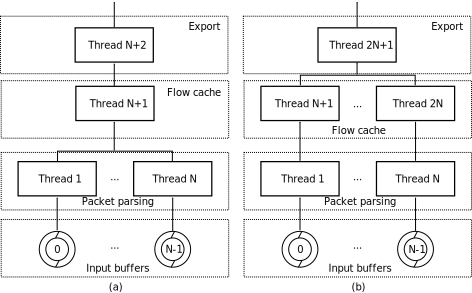
\includegraphics[width=\textwidth]{figures/exporter-thread-schema}
  \end{center}
  \caption{Multithreaded flow measurement with separate flow cache: a) single flow cache; b) multiple flow caches.}
  \label{fig:exporter-thread-schema}
\end{figure}

Separating packet parsing from flow cache management increases performance, however, processing application protocols may require a state of the connection to be kept. In such a case the flow cache record must be made available to the packet processing thread, which results in a use of synchronization primitives and overall performance decrease. One possible solution to this problem is to keep a different, smaller cache for chosen flow records directly in the packet processing thread. The only communication between the packet processing thread and the flow cache thread is a one-way passing of flow records, which can be done very effectively.

When a server with multiple CPUs is used, it is necessary to take care to assign each thread to correct CPU core. When the data is uploaded to RAM physically connected to different CPU than the packet processing core is running on, there is a performance hit for accessing the local memory of that CPU.

It is not effective to try every available application header parser on every packet to see which one is able to process it. When a packet from a flow was already matched by some application parser, it will usually not be matched by others. Therefore, by keeping the information about which flow is to be processed by each parser, most of the unnecessary and possibly expensive calls to application parsers can be eliminated. Moreover, when the flow is yet unmatched by any application parser, it is best to execute the application protocol parsers from the most common to the least common protocol.

One of the most performance critical parts of any flow measurement software is a flow cache. The cache needs to be designed to hold hundreds of thousands of flow records, do fast inserts, updates, and manage record expiration after active and inactive timeouts. It also needs to be robust and resilient enough to handle excessive workloads during DDoS attacks~\cite{Sadre-2012-Effects}. The flow cache design has been studied in the literature, for example in\cite{Wang-2011-Memory, Nassopulos-2014-Flow}. Although authors propose to use various data structures such as linked lists, trees, or multidimensional hashing table, our experience shows that the simplest solution is the best. The flow cache has to maintain data locality to make good use of CPU caches, therefore the dynamic structures do not perform as well as a simple hash table.

Flow cache inactive timeout expiration has a large impact on the performance, as shown in~\cite{Rodriguez-2013-Empirical, Molina-2006-Design}. The flow cache needs to be checked periodically to find and expire inactive records. However, doing the periodic checking in a separate thread requires extensive flow cache locking, which hinders the performance. Therefore, it is more efficient to dedicate part of the processing time of the flow cache thread itself to search for the inactive records. Carefully balancing the flow cache management tasks is a complex problem which offers a considerable potential for further research.

There are many other optimizations that can be performed to increase application flow monitoring performance, such as efficient flow key computation, processing packets in batches, ensuring CPU cache line alignment of flow records and so on. However, they are mostly a code micro-optimization no different from fine-tuning any other high-performance application and are out of the scope of this article.

%TODO split the anove text into the following subsections, or just have it all together
\subsection{Basic Flow Monitoring}

\subsection{Application Flow Monitoring}
\itodo{Speedup by omitting SSL/TLS processing for most application plugins}
\itodo{SW optimization: copy whole packet and parse during flow export in a separate thread - HTTP}




\section{High-Density Flow Monitoring}\label{sec:performance-high-density}
\itodo{TODO: Put in paper from IM2015}
\itodo{Say which throughput measurement method is used (sec 1)}
\itodo{What happens when processing is too slow? Which packets are dropped?}
\itodo{Measurement interference on 10x10G, need to drop on DMA, not input}

\section{Summary}\label{sec:performance-summary}

\chapter{Measurement of Encrypted Traffic} \label{chap:measurement-of-encrypted-traffic}

\begin{chapintro}

The application flow monitoring relies heavily upon the ability to observe and process data from application layer. However, users and companies are becoming more privacy conscious and the use of encryption is steadily increasing. This chapter presents an overview of current approaches for the classification and analysis of encrypted traffic. The contribution of our work is four-fold. First, we describe several of the most widely used encryption protocols to show their packet structure and standard behaviour in a network. This information forms the basis of all classification protocols which use either a specific packet structure or a communication pattern to identify the protocol. Second, we investigate what information is provided by these encryption protocols. Most protocols negotiate encryption algorithms in clear-text, these data can be monitored, e.g., to reveal the use of weak ciphers. Third, we describe how the structure of encryption protocols can be used to detect these protocols in a network. Traffic classification algorithms using such information are presented and we describe several open-source tools which implement these algorithms. Fourth, we provide an extensive survey of behaviour-based methods for encrypted traffic classification. We show that surprisingly detailed information can be obtained using these methods. In specific cases, even the content of the encrypted connection can be established.

The article included in this chapter is~\cite{Velan-2015-Survey}.

The organisation of this chapter is as follows:
\begin{itemize}
  \item Section~\ref{sec:enc-motivation} provides motivation for this chapter and defines its goals.
  \item Section~\ref{sec:traffic-description} explains the principles of several widely used encryption protocols.
  \item Section~\ref{sec:extraction} describes what information can be obtained from encrypted traffic using specific knowledge of the encryption protocols.
  \item Section~\ref{sec:taxonomy} describes the traffic classification taxonomy used in this chapter.
  \item Section~\ref{sec:payload-classification} describes traffic classification methods based on the specific knowledge of encryption protocols.
  \item Section~\ref{sec:detection} surveys papers on the classification of encrypted traffic using statistical and behavioural methods.
  \item Section~\ref{sec:enc-conclusions} concludes the chapter and provides directions for future research.
\end{itemize}

\end{chapintro}

\newpage

\section{Motivation and Goals}\label{sec:enc-motivation}

% Motivation
Network visibility is becoming a necessity in current networks. Security, traffic provisioning, and failure detection are the prime reasons to deploy traffic measurement. Yet, measurement has other uses and new ones are still being discovered. For instance, application performance can be measured using the data from the application layer. Information about certain applications can also be used to detect attacks and intrusions on the application level. In contrast to this, the need for protection of transmitted data and user privacy is rapidly increasing. It is for this reason that, the encryption of transmitted data is increasingly used. The ratio of encrypted traffic has recently been rising steeply as common Internet services become protected~\cite{Sandvine-2014-Global}. This change poses a challenge to currently used methods for traffic measurement, for which the identification and analysis of network traffic becomes more difficult.

Before any further analysis of encrypted network traffic can be done, the traffic needs to be identified. Statistical and behaviour-based application identification methods are less affected by encryption than deep packet inspection methods. Therefore, a lot of attention has been given to these methods, which are also considered to be privacy-conscious. However, information can event be extracted from encrypted connections, mainly from the session's initiation.

% Goal
The goal of this chapter is to provide a comprehensive overview of methods for classifying and analysing encrypted traffic. To the best of our knowledge, this is the first work which comprehensively summarizes available approaches for encrypted traffic classification and analysis. Although there has been a lot of research on traffic classification in the past decade~\cite{Dainotti-2012-Issues, Nguyen-2008-Survey, Zhang-2009-State, Callado-2009-Survey, Finsterbusch-2014-Survey}, most of the existing surveys do not explicitly consider research which targets encrypted traffic. A recent survey by Cao et al.~\cite{Cao-2014-Survey} describes the fundamentals of encrypted traffic classification. It briefly introduces recent advances and challenges in this field. However, the survey covers only a few methods of traffic classification and does not provide any comparison or assessment of these methods. Moreover, while traffic classification is an important part of network monitoring, there are other methods for analysing encrypted traffic which need to be taken into consideration. 

To achieve this goal, we have produced a survey of methods for classifying and analysing encrypted traffic in journals, conference papers, proceedings of specialized workshops and technical reports. We studied works presented in selected computer science journals, mainly the Communications Surveys \& Tutorials, Computer Networks, International Journal of Network Management and Transactions on Network and Service Management. We also surveyed international conferences such as IMC, PAM, CISDA, CNSM, IM and NOMS over the period 2005-2014. Other methods were found in references provided by the surveyed papers and in papers that referenced them.

Over the last decade, many statistical and machine learning algorithms have been applied to the problem of traffic classification. However, authors use different methodological data sets to evaluate their methods and the results are therefore not directly comparable. Most of the methods use supervised or semi-supervised machine learning algorithms to classify flows and even determine the application protocol of the flow. Most methods target encryption protocols such as SSH, SSL/TLS and encrypted BitTorrent. To describe and categorize the classification methods, we use the taxonomy of Khalife et al.~\cite{Khalife-2014-multilevel}. 


%%%%%%%%%%%%%%%%%%%%%%%%%%%%%%%%%%%%%%%% DESCRIPTION OF ENCRYPTION PROTOCOLS %%%%%%%%%%%%%%%%%%%%%%%%%%%%%%%%%%%%%


\section{A Description of Encryption Protocols} \label{sec:traffic-description}

This section provides a description of chosen encryption protocols. We selected the most widely used protocols to demonstrate the basic principles and show different approaches for secure data transport. Our choice of encryption protocols was also influenced by protocols which are the most commonly used in research of encrypted traffic classification. We shall describe IPsec, TLS, SSH, BitTorrent and Skype protocols in this section. All these protocols provide confidentiality using encryption and they usually offer authentication of communication peers, data integrity, replay protection and non-repudiation. We shall describe the use of these protocols, their fundamental properties, the structure of encrypted packets, and the type of exchanged data. The information provided in this section will serve as the basis for rest of this chapter.

Almost all the presented encryption protocols can be divided into two main phases: the initialization of the connection and the transport of encrypted data. The first phase can be further divided to an initial handshake, an authentication and a shared secret establishment. During the first phase, algorithm capabilities are usually exchanged, communication parties are authenticated and secret keys are established. These keys are then used for encrypting transferred data in the second phase. This general protocol scheme is depicted in Figure~\ref{fig:protocols-scheme}, which, with minor modifications, can be applied to almost any protocol providing confidential data transfer.

\begin{figure}[!ht]
	\begin{center}
		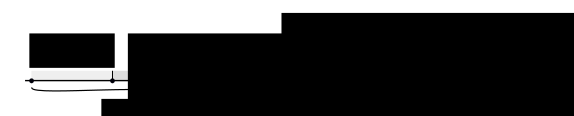
\includegraphics[width=0.9\textwidth]{figures/paper-encrypted/protocols_scheme}
		\caption{A General Scheme of Network Security Protocols.}
		\label{fig:protocols-scheme}
	\end{center}
\end{figure}

The protocols presented in this section are listed in order of their position in the ISO/OSI reference model~\cite{ISO7948-1}. IPsec protocol suite, which operates on the network layer is described first, followed by TLS and SSH protocols on the presentation layer. BitTorrent and Skype protocols represent the application layer and they implement their own protocols for secure data transmission.


%%% IPSec %%%

\subsection{Internet Protocol Security}

Internet Protocol Security (IPsec) is a framework of open standards for ensuring authentication, encryption and data integrity on the network layer. Due to its location on the network layer, IPsec can protect both the data within the packet and also L3 information (e.g., IP addresses) in each packet~\cite{SP-800-77}. The main advantage of using IPsec is securing the network connection without the necessity of modifying any application on the clients or servers. However, it provides less control and flexibility for protecting specific applications.

IPsec follows the general scheme depicted in Figure~\ref{fig:protocols-scheme}. The first phase is represented by the Internet Key Exchange Version 2 (IKEv2) protocol~\cite{rfc5996}. IPsec uses an UDP protocol on the port 500 through which all messages covering the initial handshake, the authentication and the shared secret establishment run. Two protocols could be used in the second phase of IPsec: Authentication Header (AH) and Encapsulating Security Payload (ESP). In the initial version of IPsec, the ESP protocol providing data confidentiality did not include authentication, so ESP and AH were used together. Nowadays, the current version of ESP contains authentication and AH has become less significant, although it is still used to authenticate portions of packets that ESP cannot manage.



\begin{figure}[!ht]
  \centering
  \includegraphics[width=0.9\textwidth]{figures/paper-encrypted/ipsec_transport_mode}
  \caption{The IPsec Packet Structure in the Transport Mode.}
  \label{fig:ipsec-transport-mode}
\end{figure}

\begin{figure}[!ht]
  \centering
  \includegraphics[width=0.9\textwidth]{figures/paper-encrypted/ipsec_tunnel_mode}
  \caption{The IPsec Packet Structure in the Tunnel Mode.}
  \label{fig:ipsec-tunnel-mode}
\end{figure}

The ESP protocol is the main protocol of IPsec. It provides data confidentiality, origin authentication, connectionless integrity, an anti-replay service, and limited traffic flow confidentiality~\cite{rfc4303}. ESP adds a header and a trailer to each transferred packet, see Figures~\ref{fig:ipsec-transport-mode} and~\ref{fig:ipsec-tunnel-mode}, placed according to the transport mode used. The ESP and AH protocols can operate in two modes: \textit{transport} and \textit{tunnel}. In the \textit{tunnel} mode, a new IP header is created for each packet with endpoints of the tunnel as the source and destination addresses; the original IP header is used in the \textit{transport} mode.



%%% TLS %%%

\subsection{Transport Layer Security}
Transport Layer Security (TLS)~\cite{rfc5246} is based on the Secure Sockets Layer version 3 (SSLv3) protocol~\cite{rfc6101} and provides transport level security directly on top of the TCP protocol. Specifically, it provides confidentiality, data integrity, non-repudiation, replay protection and authentication through digital certificates. The TLS is currently one of the most common protocols for securing network communication. It is mainly used for securing HTTP, FTP, SMTP sessions, as well as for Virtual Private Networks or Voice over Internet Protocol (VoIP). The protocol design is layered and consists of different sub-protocols, as well as configurable and replaceable cryptographic algorithms~\cite{tls-thesis}.

The main part of TLS is the Record Protocol~\cite{rfc5246}, which acts as an envelope for application data as well as TLS messages. In the case of the application data, the Record Protocol is responsible for dividing the data into optionally compressed fragments. The addition of fragments to the record is complemented by Message Authentication Code (MAC). For more details, see Figure~\ref{fig:tls-record}. Depending on the selected security algorithms, a fragment and MAC are encrypted together and sent as one TLS record. A packet may contain more than one record to avoid sending multiple short packets.

\begin{figure}[!ht]
	\begin{center}
		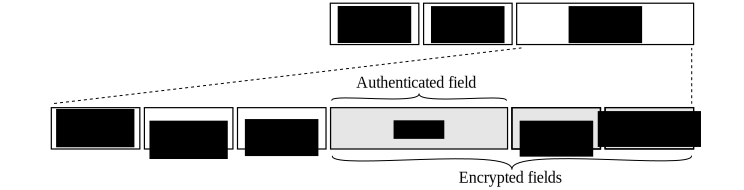
\includegraphics[width=0.9\textwidth]{figures/paper-encrypted/tls_record}
		\caption{The TLS Record Packet Format.} 
		\label{fig:tls-record}
	\end{center}
\end{figure}

During the first phase of a TLS connection, communication parties are usually authenticated (more often we can see only server authentication) using an X.509 certificates chain~\cite{rfc5280}, as shown in the general scheme in Figure~\ref{fig:protocols-scheme}. Alternatively, a previous connection can be resumed without authentication. TLS messages exchanged during this phase are unencrypted and do not contain MAC until the shared keys are established and confirmed. In the second phase, these keys are used directly by the Record Protocol, which is based on the selected algorithms ensuring communication security.

%%% SSH %%%

\subsection{Secure Shell Protocol}
In a similar fashion to the TLS protocol, the Secure Shell (SSH) protocol~\cite{rfc4253} exists as a separate application on top of TCP. This protocol uses a client-server model where the server usually listens to the TCP port 22. SSH was originally designed to provide a remote login access to replace unsecured Telnet connections. Nowadays, it can be used not only for a remote login and a shell, but also to allow file transfers using the associated SSH File Transfer Protocol (SFTP)~\cite{sftp-draft} and a Secure Copy (SCP)~\cite{scp-description} protocol, or by Virtual Private Networks (VPN). The SSH protocol provides user and server authentication, data confidentiality and integrity and, optionally, compression.

\begin{figure}[!ht]
	\begin{center}
		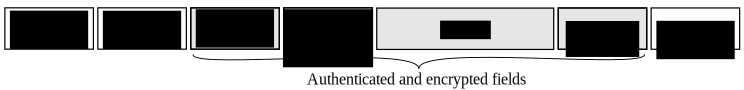
\includegraphics[width=0.9\textwidth]{figures/paper-encrypted/ssh_packet}
		\caption{The SSH protocol packet format.} 
		\label{fig:ssh-packet}
	\end{center}
\end{figure}

SSH consists of three protocols, of which the most important is the Transport Layer Protocol, which provides the establishment of the whole connection and its management. It defines the SSH packet structure, which is depicted in Figure~\ref{fig:ssh-packet}. The MAC code is computed on a plaintext payload together with the packet length, the padding and a continuously incremented sequence number not present in the packet itself. Other SSH protocols are the User Authentication Protocol and the Connection Protocol for multiplexing multiple logical communications channels~\cite{ssh-basics}.

Each SSH connection passes through the same phases which were depicted in Figure~\ref{fig:protocols-scheme}. In the first phase, a TCP connection is established and information about preferred algorithms is exchanged. During authentication, a server sends its public key which must be verified by the client (using a certification authority or manually through a different channel). The shared keys are subsequently established and confirmed. All following packets are then encrypted and authenticated.


%%% Bittorent %%%

\subsection{BitTorrent}
BitTorrent~\cite{bittorrent-specification} is an application protocol based on the principle of peer-to-peer network communication for sharing large amounts of data over the Internet. Originally, the protocol did not ensure any type of network communication security. Once the popularity of this protocol increased, some Internet Service Providers (ISP) started to limit this type of traffic. As a response to this, the Message Stream Encryption (MSE) algorithm~\cite{mse-specification}, also known as Protocol Encryption (PE), was introduced. It serves as an obfuscation algorithm to make BitTorrent traffic identification more difficult. In addition to obfuscation, the mechanism also ensures some level of confidentiality and authentication for communicating peers.

The MSE protocol specification~\cite{mse-specification} describes MSE as a transparent wrapper for bidirectional data streams over TCP which prevents passive eavesdropping and thus protocol content identification. MSE is also designed to provide limited protection against active man-in-the-middle attacks and port scanning by requiring a weak shared secret to complete the handshake. The major design goal was payload and protocol obfuscation, not peer authentication and data integrity. Thus, it does not offer protection against adversaries which already know the necessary data to establish connections (that is the IP/port/shared secret/payload protocol).

The first general phase of the MSE protocol follows a TCP three-way handshake and starts with a newly generated Diffie-Hellman (DH) public key exchange (together with random data padding for better obfuscation). The shared key is computed by the DH key and combined with hashed information about the requested data which acts as a pre-shared secret. The packet's payload is completely encrypted by a RC4 stream cipher after successfully confirming the shared key.

%%% Skype %%%

\subsection{Skype}
Skype~\cite{skype-web} is a peer-to-peer based VoIP application providing not only video chat and voice calls, but also an instant messaging and file exchange service. As the protocol used is not publicly known, it is not possible to accurately describe its specific details. The main reason for this is network data obfuscation to make the detection of Skype traffic more difficult, which is similar to the BitTorrent protocol.

The Skype protocol operates over both UDP and TCP protocols depending on network characteristics. If the network has no restrictions, the application usually sends data traffic over UDP and the signalling traffic over TCP~\cite{skype-hunter}. If UDP cannot be used (for example a firewall prevents users from using such a protocol), Skype sends both the signalling and the data traffic over TCP. When TCP is used, the connection is usually established over port 80 or 443, which masks Skype traffic as standard web traffic.

Skype uses the TLS protocol over the TCP port 443 and a proprietary protocol over port 80~\cite{skype-hunter} for securing and obfuscating generated traffic with each communicating peer. TLS is also used in communication with other Voice over IP solutions, where it is used for protecting Session Initiation Protocol (SIP) messages~\cite{skype-requirements}. Skype uses a proprietary protocol for communication over UDP. To offer a reliable connection, UDP packets contain an unencrypted header with a frame ID number and function mode fields. The encryption in UDP connections is used only for obfuscation and not for confidentiality; therefore, there is no generated shared secret, only a proprietary key expansion algorithm. UDP connections do not follow the general scheme in Figure~\ref{fig:protocols-scheme}, because encrypted data are directly transferred without an initialization phase.

%%%%%%%%%%%%%%%%%%%%%%%%%%%%%%%%%% Information Extraction from Encrypted Traffic %%%%%%%%%%%%%%%%%%%%%%%%%%%%%%%%%


\section{Information Extraction from Encrypted Traffic}\label{sec:extraction}


Network monitoring is one of the main pillars of network security. If the appropriate data is collected, it is possible to detect network attacks and trace attackers, detect security policy violations and monitor network applications performance. If encrypted traffic is used, the possibility of information extraction is significantly limited. Nevertheless, it is possible to obtain some information from this traffic, primarily from the unencrypted initialization phase, but also from the encrypted transport phase. This section begins with a description of the initialization phase, which is then followed by a description of methods which use traffic feature analysis to gain information from the transport phase.


\subsection{The Unencrypted Initialization Phase}

Almost all network protocols ensure secure data transfer by means of encryption containing an unencrypted initialization phase, as depicted in Figure~\ref{fig:protocols-scheme}. Because the data exchanged at this stage are not encrypted, they can be easily extracted and used for monitoring network traffic. Generally, two types of information common to most protocols can be extracted during this phase. The first type covers the connection itself, and its properties exchanged in the initial handshake. The second type covers communicating peers' identifiers which are exchanged in the authentication phase.

During the initial handshake, parameters of a connection are negotiated, such cipher suites and which protocol version is used. This dynamic setting of the connection properties enables backward compatibility for different versions of software or is used to set a different level of security based on established security policies. Some examples of this are data authentication and compression in addition to encryption itself. The list of possible identifications, with references to algorithm specification for IPsec, TLS, SSH and other protocols, can be found in IANA Protocol Registries~\cite{iana-protocol-registries}. All of this information can be used for proper connection characterization and correct parsing of other packets in the rest of the connection.

One interesting use of the information from the initial handshake is presented by client fingerprinting based on the provided cipher-suites. A large amount of cipher-suites types exists, which usually are not all implemented by the client's applications. Therefore, each application specifies the supported cipher-suites and also prefers using them during the initial handshake. This makes it possible to passively distinguish specific operating systems, web browsers and other applications, together with their versions, based only on the cipher-suites which they use. An example of such client fingerprinting, based on the SSL/TLS initial handshake, is presented by applications from SSL Labs~\cite{qualys-ssl-fingerprinting} and p0f module~\cite{p0f-ssl-fingerprint}.

The authentication phase represents the second source of information which can be easily extracted from secured network traffic. Unique identifiers of one or both communicating peers, optionally supplemented by additional data about them, are exchanged during this phase. For example, in the authentication phase of the SSH protocol, the server sends its public key to the user. The user must validate the key and verify that the server knows the appropriate private key~\cite{rfc4253}. Since this information is almost unique for each SSH server, it is possible to detect server changes or man-in-the-middle attacks on them by passive network traffic monitoring. 

A very good example of extracting information from communication peers is demonstrated by monitoring the authentication phase of the SSL/TLS protocol. The server, and optionally even the client, sends their X.509 certificates~\cite{rfc5280} to each other to verify their identities in this phase. This certificate contains a public key signed by the certification authority which is supplemented with information about the peer and issuer. More detailed content of such certificates is shown in Figure~\ref{fig:certificates-contents}.

\begin{figure}[!ht]
	\begin{center}
		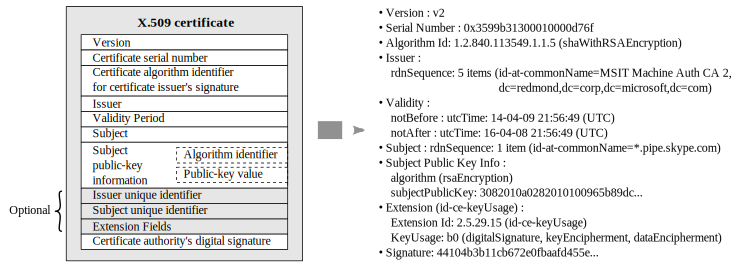
\includegraphics[width=0.9\linewidth]{figures/paper-encrypted/certificate}
		\caption{Example of Skype X.509 Certificate.}
		\label{fig:certificates-contents}
	\end{center}
\end{figure}

Monitoring passive certificates enables not only the identification of communicating peers but also the ability to check whether these certificates are valid and contains proper security algorithms to fulfil local security policies. SSL/TLS certificate properties were studied by Holz et al.~\cite{Holz-2011-SSL} who revealed a great number of invalid certificates and some which were shared between a large number of hosts. Holz et al's work was followed by Durumeric et al.~\cite{Durumeric-2013-Analysis} who mainly focused on assessing certification authorities. Certificate monitoring can also be used to detect malicious software trying to hide its activities by connecting with their command and controls centres using the SSL/TLS protocol~\cite{ssl-certificates-blacklist}.

Even though information extraction from encrypted traffic is not a computationally intensive process, it can provide valuable information. For example, extracting the Server Name Indication (SNI)~\cite{rfc4366} can be used by a home router's firewall to filter traffic. The unencrypted initialization phase is often used to recognize encrypted traffic and, the authentication information might be utilized to detect and prevent man-in-the-middle attacks on a network-wide level.

\subsection{The Encrypted Data Transport Phase}

Information about network traffic can be extracted from encrypted data which is transported between communicating parties. Packets exchanged during the transport phase usually contain only information about the packet itself, such as the length and the authentication field which are not useful for monitoring network traffic. Nevertheless, two methods do exists to obtain more suitable data. 

The first method uses direct traffic decryption, which is possible to perform only if the shared secret of the connection is known. Therefore, decryption can be used in networks on the servers' side where organizations know the private key of the connected server. However, such decryption would be impossible if algorithms wee used which ensure forward secrecy~\cite{Huang-2014-tls-forward-secrecy}. 

The second method is based on the extraction of traffic features. An example of such an analysis is presented by Miller et al.~\cite{Miller-2014-https-decrypt} who monitor the size of TLS encrypted packet sequences. Based on their data, together with various predictive models, they are able to identify a specific web page and deduce its content even though the traffic is encrypted. A similar approach was also used by Koch and Rodosek~\cite{Koch-2010-Command} for analysing SSH traffic. Another example of using traffic features is the work by Hellemons et al.~\cite{hellmons-2012-sshcure}, which focused on intrusion detection in SSH traffic. Encrypted traffic features could also be used for classifying encrypted traffic, which is described in Section~\ref{sec:detection}.


%%%%%%%%%%%%%%%%%%%%%%%%%%%%%%%%%%% Taxonomy for Traffic Classification Methods %%%%%%%%%%%%%%%%%%%%%%%%%%%%%%%%%%


\section{A Taxonomy for Traffic Classification Methods} \label{sec:taxonomy}

The first step in analysing network traffic is identifying the type of traffic measured. Network traffic classification methods are used for this purpose based on the knowledge of the protocol packet structure, communication patterns, or a combination of both.The recognition of the TLS protocol, described in Section~\ref{sec:traffic-description}, may be seen as an example of this. This protocol can be identified based on the knowledge of the packet structure, especially the unencrypted packet parts such as the content type, the version and the length. Similarly, the protocol can be identified by analysing its behaviour, e.g., the knowledge of a number and an approximate size of packets sent during the unencrypted initialization phase.

To present the current state of research on encrypted traffic classification in a comprehensive manner, we use a taxonomy of classification methods. We choose the multilevel taxonomy by Khalife et al.~\cite{Khalife-2014-multilevel}, which provides a detailed categorization of traffic classification methods. This taxonomy is uniquely descriptive and allows us to efficiently categorize all our surveyed classification methods. Figure~\ref{fig:taxonomy} shows an overview of the taxonomy levels. On the topmost level, the authors distinguish between classification input, technique and output. The input determines the traffic's characteristics, which are used for classification (e.g., packets or flows). The technique describes the core of the classification method, which may be, among others, payload inspection, a statistical method or a machine learning method. The output then describes how the traffic objects (packets or flows) map to traffic classes (application types or application protocols). The traffic classes are of a different granularity. Some methods allow identification of application protocols (e.g., HTTP), and some are more fine grained to detect, for example, a Google search or a Facebook chat.

\begin{figure}[!ht]
	\begin{center}
		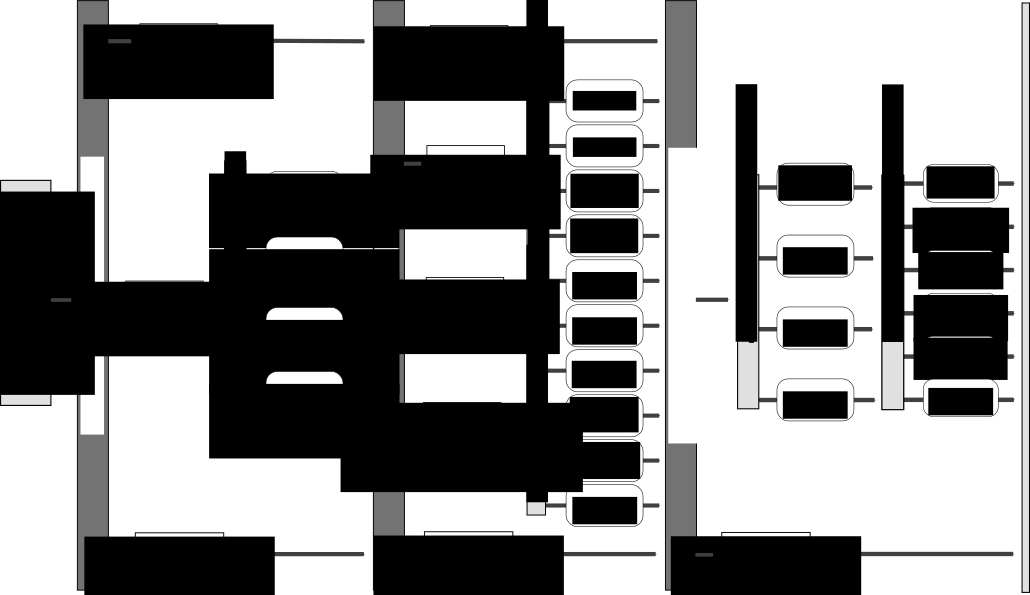
\includegraphics[width=\textwidth]{figures/paper-encrypted/taxonomy}
		\caption{A Multilevel Taxonomy of Traffic Classification Methods~\cite{Khalife-2014-multilevel}.} 
		\label{fig:taxonomy}
	\end{center}
\end{figure}

\begin{table}[!ht]
	\centering
	\small
	\renewcommand{\arraystretch}{1.05}
	\begin{tabularx}{\textwidth}{c|l|X} \hline
		\multicolumn{3}{ c }{\textbf{Classification Input}} \\ \hline \hline
		\multicolumn{2}{ c| }{\textit{Traffic Payload}} & use of application data \\ \hline
		\multirow{3}{*}{\parbox[c]{3.6cm}{\centering\textit{Traffic Properties}\\ (Measurement Level)}} & Host Community & graph metrics (diameter, connection degree) \\
		& Host & number of connections, opened ports \\
		& Flow & flow size, flow duration \\
		& Packet & packet sizes, inter-arrival times \\ \hline
		\multicolumn{2}{ c| }{\textit{Hybrid \& Miscellaneous}} & combination of inputs, external knowledge \\ \hline
	\end{tabularx}
	\smallskip
	\caption{Classification Input Level.}
	\label{tab:classification-input}
\end{table}

\begin{table}[!ht]
	\centering
	\small
	\renewcommand{\arraystretch}{1.05}
	\newcommand{\classificationsize}{2.7cm}
	\begin{tabularx}{\textwidth}{c|l|X} \hline
		\multicolumn{3}{ c }{\textbf{Classification Technique}} \\ \hline \hline
		\multicolumn{2}{ c| }{\textit{Payload Inspection}} & DPI, examination of first N bytes \\ \hline
		\multirow{3}{*}{\parbox[c]{\classificationsize}{\centering\textit{Graphical\\ Techniques}}} & Graphlets & relationship between features (ports, addresses) \\
		& Motifs & patterns of communication \\
		& Social Networks & graph of communication \\ \hline
		\multirow{3}{*}{\parbox[c]{\classificationsize}{\centering\textit{Statistical\\ Method}}} & Basic Statistical & probability density functions of e.g. packet sizes \\
		& Heuristics & port-based classification \\
		& Profiles & host profiling, usage of packet sizes and direction \\ \hline
		\multirow{3}{*}{\parbox[c]{\classificationsize}{\centering\textit{Machine Learning\\ Algorithm}}} & Supervised & Hidden Markov Models, Naive Bayes, $k$-nearest neighbour, support vector machine \\
		& Non-Supervised & clustering of unlabeled traffic, \mbox{$k$-nearest} neighbour \\
		& Semi-Supervised & clustering of mixed traffic, \mbox{$k$-nearest} neighbour  \\
		& \parbox[c]{3.5cm}{Reinforcement Learning} & - \\ \hline
		\multicolumn{2}{ c| }{\textit{Hybrid \& Miscellaneous}} & combination of methods, external knowledge \\ \hline
	\end{tabularx}
	\smallskip
	\caption{Classification Technique Level.}
	\label{tab:classification-technique}
\end{table}

\begin{table}[!ht]
	\centering
	\small
	\renewcommand{\arraystretch}{1.05}
	\begin{tabularx}{\textwidth}{c|X} \hline
		\multicolumn{2}{ c }{\textbf{Classification Output}} \\ \hline \hline
		\multicolumn{2}{ c }{\textbf{Traffic Objects}} \\ \hline
		Host Community & host community is assigned a class, e.g., community of HTTP servers \\
		Host & host is assigned a class \\
		Flow & flow is assigned a class \\
		Packets & packet is assigned a class \\ \hline \hline
		\multicolumn{2}{ c }{\textbf{Traffic Classes}} \\ \hline
		Traffic Cluster &  bulk or small transactions\\
		Application Type & game, browsing, chat \\
		Application Protocol & HTTP, HTTPS, FTP \\
		Application Software & client software such as Mail client, FTP client or web browser \\
		Fine-Grained & Skype voice call, Google search, Facebook chat \\
		Anomaly & port scan, brute-force attack \\ \hline \hline
		Hybrid \& Miscellaneous & combination of outputs or classes, external knowledge \\ \hline
	\end{tabularx}
	\smallskip
	\caption{Classification Output Level.}
	\label{tab:classification-output}
\end{table}

Tables~\ref{tab:classification-input}, \ref{tab:classification-technique} and \ref{tab:classification-output} provide examples for each of the input, technique and output category. The input and technique tables have the most general categories in the left column, some of which are divided into more specific subcategories. The classification output table is divided horizontally into traffic objects and classes. The objects describe what is being classified, in other words, whether it is each packet, whole flow or a host. Traffic classes describe the type of classification being performed by a specific algorithm.


%%%%%%%%%%%%%%%%%%%%%% Payload-Based Traffic Classification Techniques for Encrypted Traffic %%%%%%%%%%%%%%%%%%%%%


\section{Payload-Based Traffic Classification Techniques for Encrypted Traffic}\label{sec:payload-classification}


Almost every network traffic encryption protocol has a specific packet format that differs from others, as was described in Section~\ref{sec:traffic-description}. Thus, with knowledge of these formats it is possible to distinguish and identify individual protocols by inspecting the packet payload. It is for this purpose that, string or regular expression matching algorithms are used witch a specific protocol patterns. Some examples of contemporary classification tools which use payload inspection are discussed in more detail in the first part of this section. The second part presents current research papers which focus on comparing these tools in terms of their performance and success rate.


\subsection{Payload-Based Classification Tools}

Most network traffic classification tools address all network protocols and not only the encrypted ones. The following examples represent the most widely used tools for classifying network traffic. Most of these tools are also able to distinguish specific network applications, mainly in unencrypted traffic. In terms of the taxonomy, these tools mostly use the \textit{Payload Inspection} technique on the \textit{Traffic Payload} classification input to map \textit{Flows} to \textit{Application Protocols}.

\textit{PACE}~\cite{pace} is a commercial classification library written in C, which uses pattern matching augmented by heuristics, behavioural and statistical analysis. In addition to standard protocol and application recognition, it is able to identify obfuscated protocols such as BitTorrent or Skype. According to its website, PACE is able to identify thousands of network applications and protocols.

\textit{Cisco Network Based Application Recognition (NBAR)}~\cite{CiscoSystems--Network} is another example of a commercial tool for classifying network traffic. This tool is primarily used on Cisco routers for quality and security purposes. According to its authors, NBAR is also able to recognize stateful protocols and non-TCP and non-UDP IP protocols.

\textit{nDPI}~\cite{Deri-2014-nDPI} is an open-source classifier forked from the (currently closed) project OpenDPI, which was in turn derived from PACE. nDPI analyzes at most eight packets from each connection for classifying traffic, however each packet is examined separately. If the connection contains multiple matches, then the most detailed match is returned. For encrypted traffic recognition, nDPI contains only a SSL decoder that extracts the host name from the server certificate. Using these names, nDPI is able to identify specific network applications.

\textit{Libprotoident}~\cite{Alcock-2012-libprotoident} is an open-source C library for classifying traffic. In contrast to the previous tools, Libprotoident inspects only the first four bytes of a packet payload for each direction. This makes it much faster but reduces its detection accuracy. The classification uses a combined approach of pattern matching, payload size, port numbers and IP matching.

\textit{L7-filter}~\cite{l7-filter} is an open-source classifier for Linux which is designed to classify traffic on the application layer. The initial phase of classification is based on non-payload data such as port numbers, IP protocol numbers, the number of transferred bytes, and so forth. Payload data are analysed with regular expressions during the second phase. One disadvantage of the l7-filter is that it contains a database with old patterns which was last updated in 2011.


\subsection{A Comparison of Classification Tools}
A comparison of the presented open-source tools was introduced by Finsterbusch et al.~\cite{Finsterbusch-2014-Survey}. They prepared a data set containing the traffic of 14 different network protocols such as DNS, HTTP, BitTorrent, and SMTP(S) to compare the tools. Using this data set, they measured classification accuracy, memory usage, CPU utilization, and the number of packets required for proper classification. The comparison showed, amongst other results, that nDPI is not able to classify the BitTorrent protocol with more than a 43\,\% true positive rate, although it detects SSL/TLS with 100\,\% accuracy. The Libprotoident tool had the highest classification accuracy of the whole analysed traffic, which was able to classify DNS, HTTP, SIP and e-mail protocols with 100\,\% accuracy. Libprotoident also needs the least number of packets on average for classifying real-time traffic. Based on the comparison by Finsterbusch et al., we can say that Libprotoident is the most appropriate tool for classifying payload-based traffic, although it is more CPU intensive than the other tools.

Another comparison of the tools was carried out by Bujlow et al.~\cite{Bujlow-2015-classification}. They compared all of the previously presented tools. They prepared a publicly available data set for the comparison which contained encrypted and unencrypted network traffic from 17 application protocols, 25 network applications and 34 web services. Their results show that PACE and Libprotoident are the most accurate tools. Nevertheless, the Libprotoident tool was the only classifier able to identify all the encrypted protocols which were tested. Their results were generally very similar to those in the comparison by Finsterbusch et al.

In general, the payload-based classification tools use regular expression matching algorithms to identify the encrypted traffic. The main difference between the tools is how much data they need to examine and whether they need both directions of the connection for the classification.


%%%%%%%%%%%%%%%%%%%%%% Feature-Based Traffic Classification Techniques for Encrypted Traffic %%%%%%%%%%%%%%%%%%%%%


\section{Feature-Based Traffic Classification Techniques for Encrypted Traffic}\label{sec:detection}


This section surveys feature-based classification methods which specialize in encrypted traffic. These methods do not require any knowledge of the encryption protocol packet structure. Instead, they use specific protocol communication patterns to classify encrypted traffic. These methods are based on the specific protocol differences described in Section~\ref{sec:traffic-description}, such as packet and flow features of unencrypted initialization or the encrypted data transport phase. This approach provides greater generalization and allows these methods to work with new versions and types of encryption protocols without the modification of underlying algorithms.

The taxonomy specified in Section~\ref{sec:taxonomy} is used to describe the individual methods. Apart from the properties defined by the taxonomy, we also provide information about data sets used for evaluating these methods. This is especially important when additional evaluation is to be performed by other groups to verify the results of the authors. While the taxonomy provides a traffic class for classifying the application protocol, this is sometimes too coarse for our purposes. Most classification methods not only identify the encryption protocol, but also the underlying encrypted application protocol. As both cases belong to the application protocol traffic class, we provide further explanation in the description of each classification method.

A slight drawback of flow-based classifiers is in performing classification often after the flow has expired. This prevents the possibility of a real-time response, which has led several research groups to research real-time classification using flow-features. Their methods are also included with the others in Table~\ref{tab:method_categories} and differentiated by a column describing whether the classification is done in real-time or not.

Almost 250 discriminators (flow or packet features) are identified by Moore et al.~\cite{Moore-2005-Discriminators}, which can be used to classify flow records. The authors do not propose any specific classification method themselves, however, most of the classification algorithms use a subset of these discriminators for identifying traffic. In terms of the taxonomy, the authors provide a list of traffic features which are used to infer the category of the traffic's properties for the classification input.

Most of the feature-based traffic classification methods use statistical or machine learning methods. These methods are comprehensively described in \cite{Alpaydin-2010-Introduction}. Port-based classification was used in the past to associate applications with network connections, but the accuracy of this method is decreasing with the increased use of dynamic ports and applications evading firewalls. Despite the decreased accuracy, port numbers are often utilized as one of the packet features. Furthermore, port-based classification is still quite often used to establish a ground truth for traffic classification experiments.

For easier orientation, we present the surveyed papers grouped by the class of their traffic classification algorithm. Most of the papers employ Supervised Machine Learning Methods (Section~\ref{subsec:supervised}), Semi-Supervised Machine Learning Methods (Section~\ref{subsec:semisupervised}) and Basic Statistical Methods (Section~\ref{subsec:basic-statistical}). The rest combine more than one method and are therefore gathered in a Hybrid Methods category (Section~\ref{subsec:hybrid}). For each surveyed paper, we specify the classification technique, classification output, and the data sets used in the description of the classification process itself. Table~\ref{tab:method_categories} in Section~\ref{subsec:methods-summary} provides a summary of the papers with all of the mentioned properties properly categorized.

\subsection{Supervised Machine Learning Methods}\label{subsec:supervised}

Sun et al.~\cite{Sun-2010-Novel} propose a hybrid method for classifying encrypted traffic. First, the SSL/TLS protocol is recognized using a signature matching method. A Naive Bayes machine learning algorithm is then applied to identify the encrypted application protocol. The authors use a combination of public and private data sets to evaluate their method. Background traffic is taken from a public data set, BitTorrent, eDonkey, HTTP, FTP, Thunder and GRE application protocols. The signature based recognition of SSL/TLS protocols was tested on HTTPS, TOR, ICQ and other protocols. The identification of the underlying protocol was tested only for TOR and HTTPS protocols.
% INPUT: packet payload, flows (8 fetures)
% TECHNIQUE: [payload inspection, supervised] (naive Bayes)
% OUTPUT: flows->application protocol (in SSL/TLS)
% data set: public and private, real
% partial flow: no

Okada et al.~\cite{Okada-2011-Application} analyzed changes in flow features due to encryption. They created a training data set with HTTP, FTP, SSH, and SMTP application protocols encrypted using PPTP and IPsec tunnels. The authors assessed 49 flow features and analyzed which of them are strongly correlated in normal and encrypted traffic. The correlated features were then used to infer functions which transform the features between normal and encrypted traffic. Therefore, standard classifiers can be used to classify the traffic after the transformation. The authors verified their method using several modifications of the Naive Bayesian classifier.
% INPUT: Flow
% TECHNIQUE: MLA->Supervised (Naive Bayes)
% OUTPUT: Flow->Application Protocol
% data set: private, artificial
% partial flow: no

Arndt and Zincir-Heywood~\cite{Arndt-2011-Comparison} also concentrated on the classification of encrypted traffic and compared C4.5, $k$-means and Multi-Objective Genetic Algorithm (MOGA) to this end. The classification of the SSH protocol was used as an example in their study. The authors focused on the accuracy and robustness of the algorithms. Stability was tested using three different public and private data sets for teaching and evaluating the methods. Multiple different flow export settings were tested as well. Altogether, 46 flow features were used in the evaluation, however, a different subset was used by each algorithm. The C4.5 algorithm provided the best robustness, although the MOGA had a very low false positive rate when used on the same data set as it was trained on. The C4.5 was recommended for forensic analysis by law enforcement since it is applicable on a variety of networks.
% INPUT: Flows
% TECHNIQUE: Supervised (C4.5, $k$-means, MOGA)
% OUTPUT: application protocol (SSH, non-SSH)
% data set: private, public, real
% partial flow: no

% Summary of 4 Alshammari works:
Alshammari and Zincir-Heywood have published several papers~\cite{Alshammari-2009-Classifying, Alshammari-2007-flow, Alshammari-2009-Preliminary, Alshammari-2009-Machine, Alshammari-2010-Investigation, Alshammari-2011-Can} on traffic classification using various supervised machine learning methods. They focused on recognising SSH, Skype, and in one case, Gtalk traffic using flow features without port numbers, IP addresses or payloads. A set of 22 flow features was mostly used, although in one case the authors selected the features using genetic programming. Public data sets are used as well as a private data set generated on a test-bed network. The ground truth for public data sets was gained from port numbers, and the private data set includes the payload and was labelled with a commercial packet classification tool. The following algorithms for traffic classification were compared: AdaBoost, RIPPER, Support Vector Machine (SVM), Naive Bayes, C4.5 and Genetic Programming.

Kumano et al.~\cite{Kumano-2014-Towards} investigated real-time application identification in encrypted traffic. IPsec and PPTP encryption were applied to web, interactive and bulk transfer flows to create an evaluation data set. C4.5 and SVM algorithms were utilized to classify the application on these data sets. The authors then tested the accuracy of the classification using a different number of packets from the start of the flows. They measured the impact of using fewer packets on the flow features and proposed using features which show the least change to classify applications at an early stage.
% INPUT: Flows
% TECHNIQUE: Supervised (C4.5, SVM)
% OUTPUT: Flow->application type
% data set: private, artificial
% partial flow: 


\subsection{Semi-Supervised Machine Learning Methods}\label{subsec:semisupervised}

Bernaille and Teixeira~\cite{Bernaille-2007-Early} used traffic clustering to detect applications encrypted by SSL. Their method has three steps. First, they detected SSL connections using a clustering algorithm (Gaussian Mixture Model) on packet sizes and directions of initial packets of a connection. The first three packets and 35 clusters provide good accuracy in detecting SSL traffic. After the SSL traffic is identified, the first data packets of the connections are identified. The sizes of the data packets are used by a clustering algorithm to detect an underlying application in the third step. However, the packet sizes are modified in the last step to allow for encryption overhead. The evaluation of the proposed method is done on traffic traces from live networks and a manually generated packet trace. The data sets contain HTTP, POP3, FTP, BitTorrent and eDonkey application protocols encrypted using SSL. The authors also show that using a combination of clustering and port numbers to differentiate between applications in clusters provides better results than clustering alone.
% INPUT: packet
% TECHNIQUE: non-supervised, clustering (Gaussian Mixture Model)
% OUTPUT: flow->application protocol
% data set: custom, real, published
% partial flow: yes

Maolini et al.~\cite{Maiolini-2009-Real} identify SSH traffic and determine underlying protocols (SCP, SFTP, HTTP) using a $k$-means algorithm. Only three packet features are used: the direction, the number of bytes and the timestamps of each packet. Their private data sets are created from artificial traffic and contain HTTP, FTP, POP3 and SSH protocols. Control packets such as TCP handshake, retransmitted packets and ACK only packets are removed from statistics as they negatively affect the precision. Authors use only first 3-7 packets to achieve a real-time identification.

Backquet et al.~\cite{Bacquet-2009-Investigation, Bacquet-2011-Genetic} use a Multi-Objective Genetic Algorithm to select a flow feature subspace and parameters for a clustering algorithm which detects encrypted traffic. The second work employs a hierarchical $k$-means algorithm to increase the identification's accuracy. The authors evaluate both approaches on a private data set captured at a university campus. SSH is used as a representative of encrypted traffic and the ground truth is gained from the payload of the captured packets. Based on previous works, the authors argue that the feature selection and number of clusters highly affect the overall accuracy. Therefore, the authors selected four objectives for the genetic algorithm: cluster cohesiveness, cluster separation, the number of clusters and the amount of used flow features. The results show (a) that only 14 from a total of 38 flow features were used by the best-performing algorithm and (b) that using a hierarchical $k$-means algorithm increases the identification performance.
% INPUT: Flow (14/38selected by MOGA)
% TECHNIQUE: MLA semi-supervised ($k$-means, 13 clusters)
% OUTPUT: Flow->application protocol (SSH non-SSH)
% data set: private, real
% partial flow: no


Bar-Yanai et al.~\cite{BarYanai-2010-Realtime} combined $k$-means and $k$-nearest neighbour clustering algorithms to construct a new, real-time classifier for encrypted traffic. The resulting classification algorithm has the light weight complexity of the $k$-means algorithm and accuracy of the $k$-nearest neighbour algorithm. They claim the method is fast, accurate and robust in regard to encryption, asymmetric routing and packet ordering. A labelled data set was prepared from generated samples of the traffic and the classification of the data set was done using payloads of the packets. Flows shorter than 15 packets were removed from the data set, since real-time classification for such short flows is not of practical use. If available, the first 100 packets were used for the classification. The authors stress that their method is applicable in a real-time environment and tested their implementation on an ISP link. The application protocols classified are HTTP, SMTP, POP3, Skype, eDonkey, BitTorrent, Encrypted BitTorrent, RTP and ICQ.
% INPUT: Flow (17 features)
% TECHNIQUE: Semi-Supervised (k-NN, $k$-means)
% OUTPUT: flow->application protocol
% data set: private (real)
% partial flow: yes

Zhang et al.~\cite{Zhang-2013-Encrypted} propose an improvement to the $k$-means clustering algorithm. Using harmonic mean to reduce the impact of random initial clustering centres, the authors are able to increase the accuracy of the $k$-means clustering algorithm for classifying encrypted traffic. The authors test their approach on two data sets. The first contains only data labelled SSH and non-SSH, the second contains traffic from Skype, QQ, SSH, SSL and MSN protocols. However, the selection of the data sets and the selection of flow features used for classification were not justified in the paper.
% INPUT: Flow (20 features)
% TECHNIQUE: Semi-Supervised ($k$-means)
% OUTPUT: Application Protocol (SSH, non-SSH; Skype, QQ, SSH, SSL, MSN)
% data set: public, private, real
% partial flow: no

Du and Zhang~\cite{Du-2013-Design} used a $k$-means algorithm to discern traffic of three BitTorrent clients. Flow and packet header features, such as IP addresses, ports, numbers and the length of packets, were taken into consideration. The authors generated the traffic manually and, therefore, their data sample contains only traffic from three clients. The authors highlight that the method is fast and simple and that it can be used to identify the traffic in real-time.
% INPUT: Packet header and Flow
% TECHNIQUE: semi-supervised ($k$-means)
% OUTPUT: flow->application software
% data set: private, artificial
% partial flow: no

\subsection{Basic-Statistical Methods}\label{subsec:basic-statistical}

De Montigny-Leboeuf~\cite{DeMontigny-Leboeuf-2005-Flow} described the process of identifying traffic using flows and flow features. The author showed how to derive the flow features he uses and how to use them to identify the application type (e.g., interactive typing, data transfer) and block ciphers. Moreover, the author provides a list of recognition criteria for HTTP and HTTPS web browsing traffic, IMAP, POP, SMTP, SSH, Telnet, rlogin, FTP command and data, MSN chat and TCP audio streams. A subset of 39 traffic features was used to identify each application.
% INPUT: flow
% # of attributes: 39
% TECHNIQUE: basic statistical
% OUTPUT: flows->[application protocol, application type]
% data set: custom
% partial flow: no

Wang et al.~\cite{Wang-2011-Using} computed entropy from packet payloads and used it for classifying traffic. They differentiate between eight different traffic classes: text, picture, video, audio, Base64 encoded text, Base64 encoded image, compressed and encrypted. The entropy is computed on chunks of different lengths and the authors used a support vector machine algorithm for selecting feature. The computation of the entropy for four different chunk lengths was found to be sufficient for accuracy and performance. The most difficult task was to separate encrypted and compressed traffic. The authors provided an additional heuristic to distinguish these categories using frequencies of four-bit characters. The data sets used are manually obtained from captured network communication and processed to contain traffic from all classes.
% INPUT: Packet payload
% TECHNIQUE: Basic Statistical (entropy)
% OUTPUT: Application type
% data set: private, artificial
% partial flow: yes

Korczynski and Duda~\cite{Korczynski-2012-Classifying} designed a method called Statistical Protocol Identification to identify types of communication (voice call, SkypeOut, video conference, chat, file upload, file download) in Skype traffic. Nine flow features were selected using forward selection which evaluates how a given feature improves the classification performance. A private, artificially created data set with Skype traffic was used. Other traffic with SSL, SSH, HTTP, SCP, SFTP, VoIP, BitTorrent and other services, was used to test the robustness of the method. The authors reported high accuracy in their method, although the distinction between voice and video traffic remains a difficult problem.

Amoli and Hamalainen~\cite{Amoli-2013-real} described a Network Intrusion Detection System (NIDS) capable of detecting attacks in encrypted network traffic in real-time. The NIDS has two engines, the first one uses network change measurement to detect changes in a time-series, such as DoS and DDoS. The first engine clusters the data to lessen the load on the second engine. The goal of the second engine is to detect the bot master behind the attack. The second engine clusters the prepared data to obtain the behaviour of the attackers and compares it with historical data. The authors used the detected anomalies to identify the botnet masters.
% INPUT: Flow, Packet Header
% TECHNIQUE: [Basic statistical (change point detection), unsupervised (clustering)]
% OUTPUT: Flow->Anomaly
% data set: -
% partial flow: no

Korczynski and Duda~\cite{Korczynski-2014-Markov} proposed using stochastic fingerprints based on Markov chains for identifying application traffic in SSL/TLS sessions. The method is payload-based and uses statistical information from SSL/TLS headers. The authors tested their method on twelve representative applications such as Twitter, Skype and Dropbox. The Markov chain fingerprints are based on protocol specific distributions of packets in time. Data sets were captured from real traffic, contain only SSL/TLS traffic and were not published. The ground truth was obtained by inspecting domain names of the SSL/TLS traffic. The authors discovered that many protocol implementations differ from the RFC specification, which required them to adjust the fingerprints.

\subsection{Hybrid Methods}\label{subsec:hybrid}

\begin{figure}[!t]
	\begin{center}
		\includegraphics[width=0.9\linewidth]{figures/paper-encrypted/graphlets}
		\caption{A Visual Representation of Transport-Layer Interactions for Various Applications \cite{Karagiannis-2005-BLINC}.}
		\label{fig:graphlets}
	\end{center}
\end{figure}

Karagiannis et al.~\cite{Karagiannis-2005-BLINC} focused on host-based classification. Their method uses only information from the network level and therefore is not affected by transport layer encryption (e.g. TLS). The authors classified the behaviour of the hosts on social, functional and application levels, without access to packet payloads or headers. Each level was classified independently and a cross-level classification was performed afterwards. Particular applications were represented using graphlets, see Figure~\ref{fig:graphlets}, which are representations of the application’s behaviour. The authors then used heuristics to refine the classification. The ground truth for captured data sets was established by using a signature-based payload classification. Without using transport layer information, only the following traffic classes were identified: web, p2p, data (FTP, database), network management (DNS, SNMP, NTP), mail (SMTP, POP, IMAP), news (NNTP), chat (IRC, AIM, MSN messenger), streaming and gaming.
% INPUT: Host community, Host, Flow (transport protocol, avg packet size)
% TECHNIQUE: basic statistical, graphlets, heuristics
% OUTPUT: host->application type
% data set: custom, real
% partial flow: no

Wright et al.~\cite{Wright-2006-Inferring} worked on a classification of traffic in encrypted tunnels. Multiple flows can be wrapped in a single flow representing the encrypted tunnel. The information from the packet headers was not applicable, therefore the authors used only packet sizes, timing and communication direction. A $k$-nearest neighbour classifier was used for classification when all TCP connections in a set carried the same application protocol. When TCP connections carried different application protocols, the authors used Hidden Markov Models. The authors also demonstrated that it is possible to determine the number of flows in an encrypted tunnel. The port numbers were used to obtain a ground truth for the captured data set. The authors argue that mislabelled data only decreased the efficiency of their classification algorithm and therefore the real accuracy would be even higher than the reported one. The classifiers were able to detect the following application protocols: HTTP, HTTPS, SMTP, AIM, FTP, SSH, Telnet.
% INPUT: flow
% TECHNIQUE: k-NN, HMM
% OUTPUT: flow->application protocol
% data set: custom, real
% partial flow: no

Koch and Rodosek~\cite{Koch-2010-Command} proposed a system for detecting interactive attacks using SSH. Packet sizes, IP addresses and packet inter-arrival times were used to create clusters of packets which were likely to match a SSH command and its corresponding response. The SSH protocol was recognized based on the port number, and individual commands were identified from the clusters. Following this, sequences of commands were evaluated and possible malicious sequences were reported. The system allows for the customization of malicious sequences' definitions using a sub-goals characterization. Each sub-goal maps to a malicious event, such as data gathering or system manipulation. The results from the evaluation of the proposed method show that such identification is possible. 
% INPUT: Packet (packet size, inter-arrival times, IP addresses)
% TECHNIQUE: Statistical Method->[Basic Statical, Heuristics]
% OUTPUT: Fine-Grained (commands on SSH)
% data set: unknown
% partial flow: yes

Khakpour and Liu~\cite{Khakpour-2013-Information} used an entropy of packet payloads for classifying traffic. The authors showed how to compute the entropy of files and how to modify the formula for on-the-fly computation. Several entropy values were computed for each packet. CART and support vector machine (SVM) methods were used for a subsequent classification based on the computed values. Their results demonstrated that SVM methods provide comparable accuracy with less false positives. The authors argue that it is necessary to exclude application layer headers such as HTTP response or picture headers. The reason for this is that computing entropy on the headers leads to a bias and misclassification of a packet. Therefore, a cut-off threshold was used to strip application headers from unknown protocols. The traffic was first classified into three categories: text, encrypted or binary. The authors also postulated that the classification can be more fine-grained and they investigated the classification of application protocols. Then, they demonstrated that it is possible to determine an encryption algorithm with a higher accuracy than random guessing, which they found surprising.
% INPUT: Packet Payload
% TECHNIQUE: [Basic statistical (entropy), SVM, CART]
% OUTPUT: flow -> [application type (text, encrypted, binary), application protocol]
% data set: private, artificial, real
% partial flow: no

\subsection{A Summary of Machine Learning and Statistical Encrypted Traffic Classification}\label{subsec:methods-summary}

We have provided a summarizing overview of the feature-based traffic classification papers and methods they use in Table~\ref{tab:method_categories}. Where a method belongs to multiple categories, it is not marked as a hybrid, but all the categories are listed instead. We find this approach more descriptive than using a hybrid category as defined by the taxonomy.

\newcommand{\legendskip}{1.5cm}
\begin{sidewaystable}
	\centering
	\scriptsize
	\begin{varwidth}{\textheight}
	\renewcommand{\arraystretch}{1.1}
	\setlength{\tabcolsep}{0.6em} % less horizontal padding to fit to page
	\vfuzz=100pt % just get rid of those freaking warnings as an alternative to rewriting the whole table
	\begin{tabu}{c|[1pt] c|[1pt] l|l|l|l|l|[1pt] c|c|[1pt] l|l|l|l|l|l|l|l|[1pt] r @{$~\to~$} l|[1pt] c| c|[1pt] l|l|l|l|c}
		\multicolumn{1}{c|[1pt]}{} & \multicolumn{1}{c|[1pt]}{} & \multicolumn{5}{c|[1pt]}{} & \multicolumn{1}{c|}{} & \multicolumn{1}{c|[1pt]}{} & \multicolumn{8}{c|[1pt]}{} & \multicolumn{2}{c|[1pt]}{} & & \multicolumn{1}{c|[1pt]}{} & \multicolumn{5}{c}{} \\
				
		\multirow{3}{*}{\rotatebox[origin=r]{90}{\textbf{Reference}\hspace{38pt}}} & \multirow{3}{*}{\rotatebox[origin=r]{90}{\centering \textbf{Publication year}\hspace{13pt}}} & \multicolumn{5}{c|[1pt]}{\textbf{Input}} & \multirow{3}{*}{\rotatebox[origin=l]{90}{\textbf{Number of features}\hspace{7pt}}} & \multirow{3}{*}{\rotatebox[origin=l]{90}{\textbf{Feature selection}\hspace{17pt}}} & \multicolumn{8}{c|[1pt]}{\textbf{Technique}} & \multicolumn{2}{c|[1pt]}{\multirow{3}{*}{\textbf{Output}\vspace{23pt}}} & \multirow{3}{*}{\rotatebox[origin=l]{90}{\textbf{Encrypted proto. ident.}\hspace{-5pt}}} & \multirow{3}{*}{\rotatebox[origin=l]{90}{\textbf{Real-time ident.}\hspace{20pt}}} & \multicolumn{5}{c}{\multirow{2}{*}{\textbf{Data set}\vspace{11pt}}}\\[0.10cm]
		
		\cline{3-7} \cline{10-17} \cline{22-26}
		
		\multicolumn{1}{c|[1pt]}{} & \multicolumn{1}{c|[1pt]}{} & \multirow{2}{*}{\rotatebox[origin=l]{90}{\textbf{Traf. Payload}\hspace{15pt}}} & \multicolumn{4}{c|[1pt]}{\textbf{Traf. Properties}\bigstrut} & \multicolumn{1}{c|}{} & \multicolumn{1}{c|[1pt]}{} & \multirow{2}{*}{\rotatebox[origin=r]{90}{\textbf{Payload Ins.}\hspace{14pt}}} &\multirow{2}{*}{\rotatebox[origin=r]{90}{\textbf{Graphlets}\hspace{22pt}}} & \multicolumn{2}{c|}{\textbf{Statis.}} &	\multicolumn{3}{c|}{\textbf{Machine}} & \multicolumn{1}{c|[1pt]}{\multirow{2}{*}{\textbf{Method(s)}\vspace{-33pt}}} & \multicolumn{2}{c|[1pt]}{} & & \multicolumn{1}{c|[1pt]}{} & \multirow{2}{*}{\rotatebox[origin=l]{90}{\textbf{Public}\hspace{40pt}}} & \multirow{2}{*}{\rotatebox[origin=l]{90}{\textbf{Private}\hspace{38pt}}} & \multirow{2}{*}{\rotatebox[origin=l]{90}{\textbf{Real}\hspace{47pt}}} & \multirow{2}{*}{\rotatebox[origin=l]{90}{\textbf{Artificial}\hspace{31pt}}} & \multirow{2}{*}{\parbox[c]{1.4cm}{\textbf{Ground truth}\vspace{-32pt}}} \\
		
		\cline{4-7} \cline{12-16}
		
		\multicolumn{1}{c|[1pt]}{} & \multicolumn{1}{c|[1pt]}{} & \multicolumn{1}{c|}{} & \rotatebox[origin=l]{90}{\textbf{Host Com.}\hspace{7pt}} & \rotatebox[origin=l]{90}{\textbf{Host}\hspace{1pt}} & \rotatebox[origin=l]{90}{\textbf{Flow}\hspace{1pt}} & \rotatebox[origin=l]{90}{\textbf{Packet}\hspace{1pt}} & \multicolumn{1}{c|}{} & \multicolumn{1}{c|[1pt]}{} & \multicolumn{1}{c|}{} & \multicolumn{1}{c|}{} & \rotatebox[origin=l]{90}{\textbf{Basic}} &	\rotatebox[origin=l]{90}{\textbf{Heuristic}} & \rotatebox[origin=l]{90}{\hspace{1pt}\textbf{Sup.}} & \rotatebox[origin=l]{90}{\textbf{Non Sup.}}	& \rotatebox[origin=l]{90}{\textbf{Semi Sup.}} & \multicolumn{1}{c|[1pt]}{} & \multicolumn{2}{c|[1pt]}{} & \multicolumn{1}{c|}{} & \multicolumn{1}{c|[1pt]}{} & \multicolumn{1}{c|}{} & \multicolumn{1}{c|}{} & \multicolumn{1}{c|}{} & \multicolumn{1}{c|}{}  \\
		\hline\hline
		\cite{DeMontigny-Leboeuf-2005-Flow}  & 2005  & & & & \cmark & \cmark         & $\subseteq$ 39 & \xmark  & & & \cmark & & & & &                                                                          & F & AP, AT  & \xmark  &         & & \cmark & \cmark &                        & port              \\ \hline
		\cite{Karagiannis-2005-BLINC}        & 2005  & & \cmark & \cmark & \cmark &  & -- & \xmark              & & \cmark & \cmark & \cmark & & & &                                                            & H & AT      & \cmark  &         & & \cmark & \cmark &                        & signature         \\ \hline
		\cite{Wright-2006-Inferring}         & 2006  & & & & \cmark & \cmark         & 3 & \xmark               & & & & & \cmark & & \cmark & HMM, $k$-nearest neighbor                                         & F & AP      & \cmark  &         & & \cmark & \cmark &                        & port              \\ \hline
		\cite{Bernaille-2007-Early}          & 2007  & & & & & \cmark                & 3 & \xmark               & & & & & & & \cmark & Gaussian Mixture Model                                                   & P & AP      & \cmark  & \cmark  &  & \cmark & \cmark &                       & signature, known  \\ \hline
		\cite{Alshammari-2007-flow}          & 2007  & & & & \cmark &                & 22 & \xmark              & & & & & \cmark & & & AdaBoost, RIPPER                                                         & F & AT      & \cmark  &         & \cmark & \cmark & \multicolumn{2}{c|}{--}  & port, known       \\ \hline
		\cite{Maiolini-2009-Real}            & 2009  & & & & & \cmark                & 3 & \xmark               & & & & & & & \cmark & $k$-means                                                                & F & AP      & \cmark  & \cmark  & & \cmark & & \cmark                        & known             \\ \hline
		\cite{Alshammari-2009-Machine}       & 2009  & & & & \cmark &                & 22 & \xmark              & & & & & \cmark & & & \parbox[c]{2.4cm}{AdaBoost, RIPPER, SVM,\\ Naive Bayes, C4.5}\bigstrut   & F & AP      & \xmark  &         & \cmark & \cmark & \cmark &                 & port, signature   \\ \hline
		\cite{Alshammari-2009-Preliminary}   & 2009  & & & & \cmark & \cmark         & $\subseteq$ 30 & \xmark  & & & & & \cmark & & & RIPPER, C4.5                                                             & F & AT      & \xmark  &         & & \cmark & \cmark & \cmark                 & signature, known  \\ \hline
		\cite{Alshammari-2009-Classifying}   & 2009  & & & & & \cmark                & 39 & \cmark              & & & & & \cmark & & & AdaBoost, C4.5, Genetic Programming        & F & AP      & \xmark  &         & & \cmark & \cmark &                        & signature, port   \\ \hline
		\cite{Bacquet-2009-Investigation}    & 2009  & & & & \cmark &                & 38 & \cmark              & & & & & & & \cmark & $k$-means, Genetic Programming                                           & F & AP      & \xmark  &         & & \cmark & \cmark &                        & signature         \\ \hline
		\cite{Alshammari-2010-Investigation} & 2010  & & & & \cmark & \cmark         & 22 & \xmark              & & & & & \cmark & & & AdaBoost, C4.5, Genetic Programming        & F & AP      & \cmark  &         & & \cmark & \cmark & \cmark                 & signature, known  \\ \hline
		\cite{BarYanai-2010-Realtime}        & 2010  & & & & \cmark &                & 17 & \xmark              & & & & & & & \cmark & $k$-nearest neighbor, $k$-means                                          & F & AP      & \xmark  & \cmark  & & \cmark & \cmark &                        & signature, known  \\ \hline
		\cite{Sun-2010-Novel}                & 2010  & \cmark & & & \cmark &         & 6 & \xmark               & \cmark & & & & \cmark & & & Naive Bayes                                                       & F & AP      & \cmark  &         & \cmark & \cmark & \cmark &                 & known             \\ \hline
		\cite{Koch-2010-Command}             & 2010  & & & & & \cmark                & -- & \xmark              & & & \cmark & \cmark & & & &                                                                   & F & FG      & \xmark  & \cmark  & \multicolumn{4}{c|}{--}                    & --                \\ \hline
		\cite{Bacquet-2011-Genetic}          & 2011  & & & & \cmark &                & 38 & \cmark              & & & & & & & \cmark & (hierarchical) $k$-means                                                 & F & AP      & \xmark  &         & & \cmark & \cmark &                        & signature         \\ \hline
		\cite{Wang-2011-Using}               & 2011  & \cmark & & & &                & 7 & \cmark               & & & \cmark & & & & & Entropy                                                                  & F & AT      & \cmark  & \cmark  & & \cmark & & \cmark                        & known             \\ \hline
		\cite{Okada-2011-Application}        & 2011  & & & & \cmark &                & 49 & \cmark              & & & & & \cmark & & & Naive Bayes                                                              & F & AP      & \cmark  &         & & \cmark & & \cmark                        & known             \\ \hline
		\cite{Arndt-2011-Comparison}         & 2011  & & & & \cmark &                & $\subseteq$ 46 & \cmark  & & & & & \cmark & & & C4.5, $k$-means, MOGA                                                    & F & AP      & \xmark  &         & \cmark & \cmark & \cmark &                 & signature, port   \\ \hline
		\cite{Alshammari-2011-Can}           & 2011  & & & & \cmark & \cmark         & 61 & \cmark              & & & & & \cmark & & & AdaBoost, C4.5, Genetic Programming        & F & TP      & \xmark  &         & \cmark & \cmark & \cmark &                 & signature, port   \\ \hline
		\cite{Korczynski-2012-Classifying}   & 2012  & & & & \cmark &                & 9 & \cmark               & & & \cmark & & & & & Statistical Protocol Identification                                      & F & AP      & \cmark  &         & & \cmark & & \cmark                        & known             \\ \hline
		\cite{Zhang-2013-Encrypted}          & 2013  & & & & \cmark &                & 22 & \xmark              & & & & & & & \cmark & $k$-means                                                                & F & AP      & \xmark  &         & \cmark & \cmark & \cmark &                 & signature         \\ \hline
		\cite{Du-2013-Design}                & 2013  & & & & \cmark & \cmark         & 7 & \xmark               & & & & & & & \cmark & $k$-means                                                                & F & AS      & \xmark  &         & & \cmark & & \cmark                        & known             \\ \hline
		\cite{Khakpour-2013-Information}     & 2013  & \cmark & & & &                & 10 & \cmark              & & & \cmark & & \cmark & & & Entropy, SVM, CART                                                & F & AT, AP  & \cmark  &         & & \cmark & \cmark & \cmark                 & known             \\ \hline
		\cite{Amoli-2013-real}               & 2013  & & & & \cmark & \cmark         & 23 & \xmark              & & & \cmark & & & \cmark & & Change point detection, Clustering  & F & A       & \xmark  &         & \multicolumn{4}{c|}{--}                    & --                \\ \hline
		\cite{Kumano-2014-Towards}           & 2014  & & & & \cmark &                & 29 & \cmark              & & & & & \cmark & & & C4.5, SVM                                                                & F & AT      & \cmark  & \cmark  & & \cmark & & \cmark                        & known             \\ \hline
		\cite{Korczynski-2014-Markov}        & 2014  & \cmark & & & & \cmark         & -- & \xmark              & & & \cmark & & & & & Markov chains                                                            & F & AP      & \cmark  &         & & \cmark & \cmark &                        & signature         \\ \hline
	\end{tabu}
	\renewcommand{\arraystretch}{1.000}
	\begin{center}
	\begin{tabular}{lll@{\hskip \legendskip}ll@{\hskip \legendskip}ll@{\hskip \legendskip}ll}
% 		&&&&&&&& \\
		\multirow{2}{*}{\textbf{Output column legend:}\hspace{20pt}} & A & Anomaly & AP & Application Protocol & AS & Application Software & T & Application Type \\
		& H & Host & F & Flow & FG & Fine-Grained & TP & Traffic Payload \\
% 		&&&&&&&& 
	\end{tabular}
	\end{center}
	\end{varwidth}
	\caption{A summary table of cited papers and methods they use to detect encrypted traffic.}
	\label{tab:method_categories}
\end{sidewaystable}

Most surveyed methods use flow or packet header features as an input for the classification techniques. The authors of~\cite{Alshammari-2009-Preliminary, Alshammari-2011-Can} compare the results gained by utilizing packet header features and flow features. They show that using both sets of features can result in faster and more accurate classification algorithms. Nevertheless, using all the available traffic features does not necessarily lead to the best classification performance as demonstrated by the authors of~\cite{Alshammari-2009-Classifying}.

The column \emph{Number of features} shows how many flow or packet header features were used in each method. Some methods used different subsets of the features for different algorithms, and this is denoted by the $\subseteq$ mark. Moreover, some of the methods used a feature selection algorithm to select the best combination of features from the entire feature set. These methods are marked in the \emph{Feature selection} column. For this case, the \emph{Number of features} column represents the initial number of features.

Most classification algorithms are based on machine learning. The category of supervised machine learning algorithms is represented by Hidden Markov Models, RIPPER, AdaBoost, Support Vector Machines, C4.5 and Naive Bayes. Several works~\cite{Alshammari-2007-flow, Alshammari-2009-Machine, Alshammari-2010-Investigation, Alshammari-2011-Can} compare these algorithms to establish which is the best for the task of classifying traffic. The C4.5 algorithm performs the best in several cases, however, genetic programming is reported to achieve the best results in~\cite{Alshammari-2011-Can}. The second most common algorithm category is the semi-supervised machine learning, which is dominated by clustering algorithms. The $k$-means algorithm is the most frequent in this category, and the $k$-nearest neighbour comes second. The popularity of $k$-means is due to its variability, which allows it to be fine-tuned for various purposes. It is often combined with genetic algorithms to find the best setting. The authors of~\cite{Wang-2011-Using, Khakpour-2013-Information} use the entropy of packet payloads to classify traffic. Using simple statistical properties of the traffic is the third most common classification method. Other methods are rarely used, mainly because they cannot learn from labelled traffic and therefore require too much effort to set up.

The SSH protocol is heavily used as a classification example. The authors of~\cite{Alshammari-2009-Classifying, Alshammari-2007-flow, Alshammari-2009-Preliminary, Alshammari-2009-Machine, Alshammari-2011-Can, Arndt-2011-Comparison, Bacquet-2009-Investigation, Bacquet-2011-Genetic, Zhang-2013-Encrypted} test their methods for recognising SSH and non-SSH traffic. Maiolini et al.~\cite{Maiolini-2009-Real} take the classification one step further and identify the type of traffic encapsulated in a SSH connection. The authors of~\cite{Bernaille-2007-Early, Korczynski-2014-Markov, Sun-2010-Novel} use SSL/TLS traffic and identify underlying application protocols. Since the SSL/TLS protocol is more general and is used to encrypt various types of traffic, the complexity of identification is higher than for SSH. Another very popular protocol for identification is Skype, which is addressed by the authors of~\cite{Alshammari-2009-Machine, Alshammari-2011-Can, Korczynski-2012-Classifying, Korczynski-2014-Markov}.

Some of the methods focus only on identifying encrypted traffic, whereas others try to identify the underlying application protocol. The methods which perform a more thorough analysis to gain information about the application protocol are indicated in the column \emph{Encrypted protocol identification.}

Because all methods, with the exception of~\cite{Karagiannis-2005-BLINC}, classify whole flows and rely mostly on flow features, they are rarely able to classify traffic in real-time. However, the authors of~\cite{BarYanai-2010-Realtime, Bernaille-2007-Early, Kumano-2014-Towards, Maiolini-2009-Real, Wang-2011-Using} achieved near real-time classification by extracting features of only a fixed number of packets in a flow. They argue that the first packets carry enough information for classification. Using a higher number of packets increases accuracy, therefore it is possible to strike a balance between accuracy and early identification.

The \emph{Data set} columns describe whether the data used to evaluate the presented methods was taken from a live network (Real) or generated by a tool (Artificial). We also identify if the data sets were publicly available (Public), were made available by the authors (Published) or kept undisclosed as they contain sensitive information (Private). If more than one data set was used for each evaluation, we simply performed an union of the data set descriptions. The \emph{Ground truth} column indicates how the ground truth was obtained for each data set. Common methods are based on port numbers or signatures, which use the packet payload. When the data sets are generated manually, the ground truth is known in advance.

The classification accuracy reported by authors of the surveyed methods depends heavily on the data sets used. All authors use their own private data sets which are seldom published. Such methods simply cannot be compared without repeating the experiments on a common data set. The authors of~\cite{Alshammari-2007-flow, Alshammari-2009-Machine, Alshammari-2011-Can, Arndt-2011-Comparison, Sun-2010-Novel, Zhang-2013-Encrypted} also used publicly available data sets which were either labelled beforehand, using payload when available, or simply labelled using port numbers. A combination of data sets is often used to test the robustness of the methods. 

The surveyed methods show that a lot of effort was put into classifying encrypted traffic. We believe that there are several points that should be taken into account in any future research in this field. First, identifying encrypted traffic is not enough. The identification of the underlying protocol is the real challenge. Second, a SSL/TLS protocol should be used as the reference protocol, as it can contain much more complex traffic than the SSH protocol. Finally, the traces used should be labelled and made available to other researchers. Following these points does not limit the scope of future research, however, it simplifies the comparison of the presented approaches and allows others to verify the results more easily.


%%%%%%%%%%%%%%%%%%%%%%%%%%%%%%%%%%%%%%%% CONCLUSIONS %%%%%%%%%%%%%%%%%%%%%%%%%%%%%%%%%%%%%%%%%%%%%%%%%%%%%%%%%%%%%


\section{Conclusions} \label{sec:enc-conclusions}

In this chapter we presented an overview of current approaches for the classification and analysis of encrypted traffic. First, we selected a number of the most widely used encryption protocols and described their packet structure and standard behaviour in a network. Second, we focused on information which is provided by encryption protocols themselves. We found that the initiation phase often provides information about the protocol version, ciphers used, and the identity of at least one communicating party. Such information can be used to monitor and enforce security policies in an organization. We also discovered that the use of information from the unencrypted parts of an encrypted connection for a network anomaly detection is only briefly investigated by researchers. Information about communicating parties can be leveraged to discern the type of encrypted traffic. For example, the list of supported cipher suites provided by a client when establishing a secure connection can help to identify the client. We believe that the use of unencrypted parts from the initiation of an encrypted connection should be explored in more detail.

Before starting the analysis of the encrypted network traffic, it is necessary to identify it. Thus, we surveyed approaches to classifying network traffic. These, were, first payload-based methods which use knowledge of a packets' structure and feature-based methods which use characteristics specific to the protocol flow. For the payload-based classification, there are several open-source traffic classifiers which can identify encrypted traffic using pattern matching. The initiation of a communication often has a strictly defined structure, therefore, the patterns can be constructed for specific protocols. The main difference between various classifiers is that some of them require traffic from both directions of the communication to correctly classify the flows.

Feature-based traffic classifiers have been intensively researched over the last decade. Many statistical and machine-based learning methods have been applied to the task of traffic classification. Despite this, there are no conclusive results to show which method has the best properties. The main reason is that the results depend heavily on the data sets used and the configuration of the methods. We have applied the multilevel taxonomy of Khalife et al.~\cite{Khalife-2014-multilevel} and categorized existing methods. Our results show that most of the authors use private data sets, sometimes in combination with public ones. For this reason, the individual results are not directly comparable. Most of the methods use supervised or semi-supervised machine learning algorithms to classify flows and even determine the application protocol of a given flow. Most methods target encryption protocols, such as SSH, SSL/TLS and encrypted BitTorrent, and use similar methods. However, there are also some novel works which apply innovative approaches to refine the classification up to deriving the content of the encrypted connections.

Most authors of feature-based classification methods claim that their approach is privacy sensitive as it does not require the traffic payload. However, privacy issues are much wider. In 2013, the Cyber-security Research Ethics Dialog \& Strategy Workshop~\cite{CAIDA-2013-Cyber} started a discussion about the influence of cyber-security research on the privacy of Internet users. Researchers need to keep in mind that their research activities have a significant impact on infrastructure security, network neutrality and privacy of end users. 

In the past, internet protocols were not designed with security considerations in mind. The recent interest in privacy has motivated the IETF to reconsider this approach and discuss the privacy aspects of the protocols. Discussions held in~\cite{IETF-2014-IETF} revealed that monitoring privacy issues are of great concern. This discussion resulted in a new RFC~\cite{rfc7258}, where the IETF clearly states that pervasive monitoring is considered to be an attack. The document suggests that the IETF's protocols should be hardened against such monitoring. It is clear that the struggle between the demand for privacy and the need for security is still beginning.



\chapter{Next Generation Flow Monitoring}\label{chap:next-generation-flow}

\begin{chapintro}



% cca 250 words

The paper included in this chapter is~\cite{Velan-2016-EventFlow}.

The organisation of this chapter is as follows:
\begin{itemize}
  \item Section~\ref{sec:ng-background}
  \item Section~\ref{sec:eventflow} 
  \item Section~\ref{sec:metaflow} 
  \item Section~\ref{sec:app-events} 
  \item Section~\ref{sec:ng-summary} summarizes the chapter.
\end{itemize}

\end{chapintro}

\newpage


\section{Background}\label{sec:ng-background}
% TODO mozna nebude potreba, ale bude se hodit v intru, pripadne v zaveru
\itodo{Popsat milniky flow monitoringu - pocatky, security, application visibility, high-speed, ...\\
Ukazat, kam se muze flow dostat dal - eventflow, metaflow, application event\\
timeline obrazek}

\section{EventFlow}\label{sec:eventflow}

%% motivation
Application flow monitoring parses data from application headers and adds application specific elements to flow records. This way the information from application level can be easily transferred to flow collectors, stored, and utilised together with the information about the network communication. Current approach is to treat separate application protocols individually, e.g., develop an application processing module for each monitored protocol, as shown in Chapter~\ref{chap:application-flow-monitoring}. However, connections between different protocols are lost in this scenario. For example, when a~user wants to access a~web page, several different flows records are created. The DNS server must be contacted to resolve the hostname of the web page to an IP address. After the basic document is loaded, the user's browser automatically loads linked content, such as images, cascading style sheets, and java script libraries. The generated requests are recorded as flows, however, little relation between the flows is preserved.

Information about relations between individual flows can be useful in several scenarios. First, when an advertisement on a web page contains malware, the page can be traced using the relation and notified of the malicious content. Second, aggregates of the related flows can be created to simplify behavioural analysis of network traffic. Moreover, the analysis can use the additional information to improve its accuracy. Last, traffic classification engines can also benefit from having access to information about flow relations~\cite{Wang-2014-Internet}.

%% goals
In this section we present a~flow monitoring extension, called EventFlow, which allows to keep track of relations between HTTP and DNS application flows. Information about flow relation is inserted to flow records to keep track of individual user actions, i.e., events. We develop a~prototype of the EventFlow extension and evaluate its properties on network traffic trace from an ISP network. Results show that at least 10\,\% of HTTP and DNS flow records form more complex events. We believe, that this is only a~lower bound and that further improvements can be made to relate even more flows into events.

The rest of the section is structured as follows. Related work is surveyed in Subsection~\ref{subsec:eventflow-related_work}. We propose the architecture of EventFlow measurement in Section~\ref{subsec:eventflow-architecture}. Subsection~\ref{subsec:eventflow-prototype} describes the implementation of the EventFlow prototype. Experimental evaluation of the EventFlow prototype is performed in Subsection~\ref{subsec:eventflow-evaluation}. The section is concluded in Subsection~\ref{subsec:eventflow-conclusions}.


\subsection{Related Work} \label{subsec:eventflow-related_work}

Madhyastha and Krishnamurthy~\cite{Madhyastha-2008-Generic} propose a~generic language for application-specific flow sampling. Their language allows applications to select flows with special properties so that the negative impact of sampling on these applications is minimised. This can be useful for intrusion detection systems or traffic classification applications. Although the goal of this work is different from ours, it also aims to improve the collected data, so that traffic analysis applications can achieve higher accuracy.
% language for app-specific flow sampling
% better flow sampling, applications can say what they need
% allows to select flows with special properties -> ease of processing for end applications such as IDS or traffic classification applications.

The authors of~\cite{Lee-2015-Flow} also focus on improving quality of sampled flow data. They show that the traffic classification accuracy can be increased using related sampling, which assigns higher probability to connections that are part of the same application. The authors propose to use a~source IP address as a~measure of relation between connection sessions.
% sampling based on flow relation - same IP address
% more flow per application session 
% better classification accuracy

Hu et al.~\cite{Hu-2009-Entropy} propose an entropy based aggregation system to mitigate an impact of DoS attacks and worm spreads on a~network monitoring system. The main contribution of their approach is a~flow key attribute selection algorithm that chooses key attributes by which the flows are aggregated. Two dimensional hash table is used to implement their approach. The aggregated flows are called metaflows. The main difference from EventFlow is that we label existing flows belonging to same user action, while the metaflow is a~substitute flow for many flows created during a malicious network activity.
% aggregation to metaflows in case of DoS or worm spread
% the most important part is selection of flows to aggregate and appropriate key attributes for the aggregation
% two dimensional hash table

Dolberg et al.~\cite{Dolberg-2012-Efficient} introduce a~multidimensional flow aggregation aimed to reduce the volume of collected data. The authors use tree structures for storing the data by chosen dimension such as IP addresses or ports. EventFlow proposed in our work might be used in this scenario to aggregate flows by the same events.
% multi-dimensional aggregation of stored information
% reducing the amount of data
% using tree structures
% has a few relevant aggregation citations

% Removed for the lack of space
The usual approach to reduce the volume of collected data is to use sampling. Estan et al.~\cite{Estan-2004-Building} propose to use adaptive sampling rate to achieve highest possible accuracy within given data collection constrains. Their main contribution is a system for renormalisation of flow entries after the sampling rate was changed. The authors propose an extension to standard flow counting that increases the accuracy of the counters for sampled flow.
% adaptive sampling rate
% renormalization of flow entries after sampling rate change by manipulating packet and byte counters in existing entries


\subsection{EventFlow Architecture} \label{subsec:eventflow-architecture}

This section describes the architecture of the EventFlow monitoring. The goal is to label all flows that are the results of a~single user action with the same event identifier (EID). For example, accessing \url{http://www.w3.org/} creates 1 DNS request, 37 HTTP requests, and 8 HTTPS requests. We aim to assign a~single unique EID to the flows generated for all these DNS and HTTP requests.

\begin{figure}[!tb]
    \centering 
    \includegraphics{figures/paper-eventflow/dependencies}
    \caption{Relations between HTTP and DNS Requests and Responses.}
    \label{fig:eventflow-relations}
\end{figure}

Four basic types of flows are recognised by the EventFlow: HTTP requests, HTTP responses, DNS requests and DNS responses. There are relations between these types of flows in network traffic, as shown in Figure~\ref{fig:eventflow-relations}. When HTTP request to a~new site is performed, the IP address of the site must be resolved first. Therefore, a~DNS request is created. After the request is observed, a~reply usually follows, which results in the relation 1). After the DNS reply arrives, the client knows the IP address of the server and makes the HTTP request, which creates the relation 2). An HTTP response follows the request, as indicated by the relation 3). The HTTP response can contain an HTML page which links to several additional resources such as external style sheets or images. The loading of these resources triggers more HTTP requests, resulting in relation 4). When these requests point to previously unresolved domains, new DNS requests are created, which introduces the relation 5).

We base the EventFlow architecture on the relations between the requests and responses. When an HTTP or a~DNS flow is encountered, we must make sure that it is assigned the same EID as the related flows. Therefore, we create four sets of records: expected HTTP requests, expected HTTP responses, expected DNS requests and expected DNS responses. When processing an HTTP or a~DNS flow, we add new record to the set or sets it relates to. Then, when a~next flow is processed, it is matched against appropriate expected set to see whether it is a~part of existing event. If it is, an EID of the event is assigned to the flow record. For example, when a~DNS response is encountered, a~new record is put into the expected HTTP requests set (because of relation 2), see Figure~\ref{fig:eventflow-relations}). Then, when an HTTP request is processed, we check the expected HTTP requests set to see whether we are expecting this request based on a~previous DNS response. If the request is matched, it is assigned the same EID as the DNS response. 

\begin{table}[!t]
        \caption{Matched Flow Properties.}
        \centering
        \renewcommand{\arraystretch}{1.1}
        \begin{tabular}{l|c|c|c|c|c|c}
                         & \rotatebox[origin=r]{90}{\centering \textbf{Source IP}\hspace{33pt}} 
                         & \rotatebox[origin=r]{90}{\centering \textbf{Destination IP}\hspace{19pt}} 
                         & \rotatebox[origin=r]{90}{\centering \textbf{Destination Port}\hspace{9pt}} 
                         & \rotatebox[origin=r]{90}{\centering \textbf{URL}\hspace{48pt}} 
                         & \rotatebox[origin=r]{90}{\centering \textbf{Domain}\hspace{39pt}} 
                         & \rotatebox[origin=r]{90}{\centering \hspace{3pt}\textbf{DNS Transaction ID}} \\ \toprule
                        Expected HTTP Request  & \cmark &  &  & \cmark & \cmark &  \\ \hline
                        Expected HTTP Reply    & \cmark & \cmark & \cmark &  &  &  \\ \hline
                        Expected DNS Request   & \cmark &  &  &  & \cmark &  \\ \hline
                        Expected DNS Reply     & \cmark & \cmark & \cmark &  &  & \cmark \\ \bottomrule
        \end{tabular}
        \label{tab:eventflow-matched-properties}
\end{table}

Each of the sets of expected records uses different flow properties to match a~flow record. When matching an HTTP request flow against the expected HTTP requests set, the source IP address of the flow must match as well as the requested domain or the URL, if available. Checking the source IP address ensures that flows from different hosts are not combined into a~single event. A~domain name is checked for the records that were inserted in the set when DNS reply was encountered. In case an HTTP response caused the record to be inserted, the full URL is available, not only the domain name. Replies are checked based on IP addresses and destination port. Source port is not checked since  the services are expected to run on standard, well-known ports. The DNS reply is also checked for transaction ID, which is a unique identifier tying the request and response. However, the DNSSEC extension is ignored and does not affect the EventFlow. Therefore, any malicious responses would still be part of an event. List of the used properties is provided in Table~\ref{tab:eventflow-matched-properties}.

An expiration of the records from the expected sets must be ensured. When a~record from any of the expected sets is matched, it is removed. However, many inserted records will never be matched. For example, when a~DNS request is made to accommodate a~different service than HTTP, the expected HTTP request might never appear. We need to free such records from the sets eventually. A~timeout is used to keep the expected sets from being congested by redundant records. A~timestamp is assigned to each record upon insertion to a~set. Then, each time the set is searched, records older than the timeout are removed. The timeout should be as short as possible to avoid blending of several events. However, it should be at least as long as it takes to process the longest user action, which might be up to a~couple of seconds in case of complicated queries to slow sites.

There are several caveats to our approach and some limitations of the architecture that should be addressed in the future. Our approach does not handle HTTP redirection codes, therefore the first request and the HTTP 3xx redirection response are assigned different EID than the subsequent request to the resource. This problem can be rectified simply by adding a~handler for the HTTP 3xx redirection responses that will put a~new record with the redirect URL to the expected HTTP requests set.

Another limitation of our approach is that the URLs are only extracted from HTML documents. However, modern web sites often use a~JavaScript code to request additional resources through the Ajax technique. Such requests cannot be easily matched to an event, since it would require to reconstruct the complete web page and process the included JavaScript code, which is infeasible for the flow monitoring system.

There are also several caveats that cannot be avoided. Some of the requested documents might be cached by clients which would cause EventFlow to lose track of related URLs. However, cached DNS queries are of no consequence to the EventFlow since no traffic is generated for them and no information about a~flow relation is lost. Actions of different users can be mingled when Network Address Translation is used. And finally, the growing deployment of HTTPS reduces the usefulness of the EventFlow for the HTTP protocol. Nevertheless, it can always be used in environments utilising an HTTPS proxy such as data centres or enterprise networks.



\subsection{EventFlow Prototype} \label{subsec:eventflow-prototype}

We build the EventFlow prototype as a~plugin for the FlowMon~\cite{FlowmonNetworks--Flowmon} flow monitoring software. The FlowMon exporter is a~flexible flow exporter that provides support for various extensions. These extensions are used to implement a support for additional packet inputs, application protocol processing and different export protocols. We utilise the capabilities of the exporter to create an EventFlow extension plugin. The prototype can either be deployed to process data on live network or to analyse captured samples.

\begin{figure}[!tb]
    \centering 
    \includegraphics{figures/paper-eventflow/prototype-schema}
    \caption{EventFlow Prototype Schema.}
    \label{fig:eventflow-prototype-schema}
\end{figure}


% how flowmon works
The FlowMon exporter consists of three main components as shown in Figure~\ref{fig:eventflow-prototype-schema}. The first component is a~packet parser. It receives packets from the network and extracts information from network to application layer of each packet. The extracted information is used to create a~partial flow record, which contains all necessary information about the parsed packet such as IP addresses, ports, timestamps, byte counter, etc. It also contains application layer information when an application parsing is performed. The partial flow record is passed to the second component of the exporter which is a flow cache. The partial record is either inserted as a~new flow record or it is used to update an existing flow record, which is an aggregation of previous partial flow records. When a~flow record expires, it is released from the flow cache to an export component. The purpose of the export component is to convert raw flow records to a flow export protocol format such as NetFlow~\cite{rfc3954} or IPFIX~\cite{rfc7011} and pass the flow records over the network for further processing.

Plugins, that extend the FlowMon exporter to process specific application layer protocols, such as DNS or HTTP, have access to several parts of the flow creation and export process. Each plugin can request to see the raw packet payload, process it, and add its own information to flow records, such as HTTP Host, Content-Type, or Response Code. Furthermore, the plugins are allowed to provide their own functionality for insert, update, and release methods of the flow cache. And last, each plugin defines how the information inserted into flow records is processed by the export component.

The EventFlow prototype is implemented as an application protocol extension. However, it also utilises the data provided by other application plugins. The EventFlow combines information from the DNS and HTTP protocols to detect relations between flows, therefore it requires the DNS and HTTP application plugins to be deployed as well. The prototype extends the packet parser to extract URLs from HTML pages. These URLs are sent together with partial flow record to the flow cache, however, they are used only internally and they are newer exported in the flow records. When a~new flow record is created in the flow cache, the expected sets (see Section~\ref{sec:architecture}) are searched for a~match to the new record using DNS, HTTP, and URL information provided in the partial record. If a~match is found, the new flow records is assigned an Event ID (8 byte unsigned integer) of the matched record from the expected sets. Otherwise, if no match is found, a new EID is incrementally assigned to the new flow record. After the flow is expired from the cache, the EID is a~part of the record and is sent by the export component along with the rest of the flow record.

Using an 8 byte integer for EID and assigning it incrementally to individual events ensures that there are no collisions due to EID overflow in practice. However, an assignment that is individual for each flow probe and persistent over the reboots of the system would be required for a~real-world deployment. The EID is assigned only to flows of the HTTP and DNS traffic, since it would provide no benefit to other flows as event relation tracking is not implemented for other protocols yet. Moreover, the size of the flows grows only by 8 bytes at maximum, which has negligible impact on the flow collector disk space requirements.


\subsection{Experimental Evaluation} \label{subsec:eventflow-evaluation}

We evaluate the prototype in two scenarios. First, we assess the functionality of the prototype on a~simple example web site. Once we have verified the functionality, we run EventFlow on a~packet trace from live network to determine how many flows can be joined to events in real traffic. The IPFIXcol~\cite{Velan-2012-Flow} flow collector is used to collect and process the generated flows. The main advantage of the collector is that it can be easily configured to work with the Event ID element.

We do not evaluate the performance of the prototype in this phase. We are aware of several performance inefficiencies that need to be solved before any valuable results can be measured. For example, one of the most expensive parts of the prototype is the management of sets of expected records. We expect that changing the underlying data structures will significantly improve the performance.

\subsubsection{Functional Evaluation}
For the first scenario, we create a~simple website with two pages, each linking the other page, displaying an image, and referencing a~different JavaScript library. The evaluation proceeds as follows. We request the first page in a~browser and few seconds after it loads we follow the link to the other page. The packet trace of these actions is recorded and processed by the EventFlow prototype, and the resulting flows are collected by the IPFIXcol.

We expect to see a~flow record for each of the requests and responses. However, due to the HTTP pipelining the whole communication with the web server hosting the test pages is done using a single connection. Therefore, there is a~pair of flows for the accessing the two web pages with the linked images (which were on the same server), two pairs of flows for each off-site JavaScript library, and three pairs of DNS flows for IP address resolution. There are 12 flows created in this test scenario in total. The 12 flows are divided in two events by the EventFlow prototype. The first event contains flows for the two DNS requests, HTTP communication with the web server and download of the first JavaScript library. The second event does not contain an HTTP flow due to the HTTP pipelining but contains the DNS request and the subsequent download of the second JavaScript library.

The functional evaluation shows that the prototype correctly recognises related flows and labels them as a~part of the same event. The flow exporter can be extended to handle HTTP pipelining by creating new flow record for each pipelined request. Such extension would make the measurement more accurate and we plan to deploy it in the future.

\subsubsection{Real Traffic Evaluation}

\begin{table}[!tb]
	\caption{Real Traffic Evaluation Statistics.}
	\centering
	\renewcommand{\arraystretch}{1.1}
	\begin{tabular}{|l|r|} \hline
		\textit{Total Flows} & 613953 \\ \hline
		\textit{HTTP Requests} & 33294  \\  \hline
		\textit{HTTP Responses} & 49753  \\  \hline
		\textit{DNS Requests} & 197926  \\  \hline
		\textit{DNS Responses} & 224588  \\  \hline
		\textit{Events with $>$ 1 Flow} & 28064  \\  \hline
		\textit{Flows in Events with $>$ 1 Flow} & 55881  \\  \hline
		\textit{All Events} & 388749 \\  \hline
		\textit{Flows in All Events} & 418671 \\  \hline
	\end{tabular}
	\label{tab:eventflow-stats}
\end{table}

The purpose of the real traffic test is to determine how many flows can be joined into events. We collect a~short (approximately one minute) trace of 10 million packets from an ISP network on ports 53 and 80 which are likely to be DNS and HTTP packets. Table~\ref{tab:eventflow-stats} shows statistics that describe the packet trace as well as the results of the evaluation. We can see that from the total number of more than 600 thousand flows more than 400 thousand are part of events. Furthermore, over 55 thousand flows are part of events which contain more than one flow. Therefore, we can conclude that more than 10\,\% of observed HTTP and DNS flows are recognised as a~part of more complex events by the EventFlow prototype.

The number of flows in complex events is not as high as might be expected given the large number of HTTP and DNS requests and responses. We believe that this is caused by a~quite short time window of our trace, which is likely to have captured large number of separate responses and requests. Moreover, we believe that better results can be achieved by fine-tuning the timeout of the records in the expected sets of the EventFlow prototype.


\subsection{Conclusions} \label{subsec:eventflow-conclusions}

We have presented an EventFlow monitoring architecture that allows to keep track of relations between HTTP and DNS application flows, which can be used to simplify behavioural analysis of network traffic, improve network threat detection and network traffic classification. The changes to existing flow monitoring architecture are negligible, which facilitates wide deployment. The relation between flows is encoded as an 8 byte unsigned integer called Event ID which is shared by the related flows. The proposed architecture can be further extended to handle more complex HTTP communication, such as redirection return codes.

A~prototype of EventFlow plugin for the FlowMon flow exporter has been evaluated on a~trace of 10 million packets. We showed that more than 10\,\% of observed HTTP and DNS flows are recognised as a~part of more complex events by our prototype. We believe that this result will improve on longer packet trace as well as with more accurate settings of the prototype. Prospective improvements to the prototype as well as its more detailed evaluation, including a~performance evaluation, are left for a~future work.

We believe that the network analysis will benefit from the supplemental information about flow relations. Our work has shown that it is possible to acquire such information without a significant impact on an existing monitoring architecture and that it is possible extend the flow monitoring to trace relations of other application protocols.

%% shortcommings
% browser caching
% dns caching -> no request, no problem
% dns might be elsewhere (but should not if it is not cached)
% urls created by javascript
% redirections HTTP codes 3xx
% https

%% results
% prototype implementation for flow exporter
% evaluation on real ISP network

%% privacy issues
% asi do nejake sekce
% strojove zpracovani HTML stranek dela dneska kazdy
% k analytikum se dostane pouze informace o souvislostech toku

% future work: addressing the javascript shortcoming, VoIP, FTP



\section{MetaFlow}\label{sec:metaflow}
% zobecneni eventflow, vice urovni toku (zanorene protokoly), i aplikacni protokoly by mohly mit svoje specificke toky (kazdy Lx protokol svuj tok, vsecko provazane)
% PAM 2018

\section{Application Events and Flow}\label{sec:app-events}
% dalsi moznosti se jevi exportovat toky a vedle nich aplikacni udalosti. nervat to primo do toku, protoze to cele ty toky rozbiji a neni to moc elegantni na zpracovani

% application events jsou hezky obecny veci, dobre by to umoznovalo kombinovat i data z logu a podobne.


\section{Summary}\label{sec:ng-summary}

% EventFlow
Network flow monitoring is being supplemented with an application flow visibility to provide more detailed information about network traffic. However, the current concept of flows does not provide a~mechanism to keep track of semantic relations between individual flows that are created as a~part of a~single user action. We propose an extension to the flow measurement, called EventFlow, which allows to preserve relations between HTTP and DNS application flows that are a~part of single user action, most typically browsing a~web page. We describe an architecture of the EventFlow extension and its limitations. A~prototype implementation of the EventFlow is introduced and evaluated on a~packet trace from an ISP network. We show that a~significant number of flow records can be recognised as a~part of a~single user action.

\chapter{Conclusion}\label{chap:conclusions}

The flow monitoring has evolved significantly in the past several years. The most substantial progress has been made in the performance  area of flow monitoring, which needed to match the development of networking toward 100\,Gbps technologies, and in processing of application layer information. This thesis has presented our contributions in both of these areas. 

\section{Research Goals}

We have established the following three research goals in the introduction of this thesis:
\begin{itemize}
  \item Propose application flow monitoring which utilizes application layer information to facilitate flow analysis and threat detection.
  \item Evaluate performance of flow monitoring and propose optimisations to facilitate monitoring of high-speed networks.
  \item Analyse options of monitoring of encrypted traffic, survey encryption protocols and methods for encrypted traffic classification.
\end{itemize}

To address the first goal, we have proposed and defined application-aware flow monitoring (i.e. application flow monitoring). We started by analysing the current definition of flow, provided an improved alternative, and formalized our definition. Based on the definition of flow, we have proposed a definition of application flow. Since the use of the terms flow, IP flow, and application flow differs in the literature, we have introduced a consistent terminology to deal with the potentially confusing differences. After that, we have described the application-aware flow monitoring system and pointed out the important differences to the basic flow. 

To show the value of application flow monitoring for traffic analysis, we have analysed four different use cases. The first, most common use case, has utilized extended information from HTTP headers to detect new classes of attack on the application layer. The second use case has shown how IPv6 tunnelled traffic can be observed and analysed with application flow monitoring. We have demonstrated that the newly acquired information helps us to better understand the network traffic. The third use case has added geolocation information to flow records to aid traffic analysis and the fourth discussed how different samples of network traffic might be compared and experiments repeated on a live networks.

Our work on the second research goal has included both application and basic flow monitoring. We have designed and implemented application flow monitoring for HTTP protocol and evaluated its performance. Multiple approaches to design of HTTP application parser were taken into consideration and utilized. By comparing results of different parser implementations, we have shown that the performance of application flow monitoring system is significantly affected by the design of application parsers. Moreover the composition of the traffic matters even more than for the basic flow as the percentage of the given application in the traffic affects the performance substantially.

We have discussed how the design of the flow monitoring process affects the performance. Performing application analysis for multiple protocols at speeds of and beyond 100\,Gbps is not possible without heavy acceleration using specialized NICs~\cite{Kekely-2016-Software} and even then depends on the traffic composition. We have build a high-density flow monitoring system, which could process traffic from sixteen 10\,Gbps links and analysed its performance. We compared settings with and without hardware acceleration for different packet sizes and different number of simultaneous flows. Our results have shown that full line rate can be achieved on real networks. We believe, that the results could be improved by applying more optimizations.

% TODO encryption

% \section{Summary of Contributions}

\section{Further Research}

\begin{itemize}
  \item 400\,Gbps and more, hardware acceleration, commodity systems
  \item Encryption - application of machine learning to flow monitoring
  \item Cloud - host based monitoring + logs
  \item Virtual environment - Open Flow - current hot topic
  \item React to demands of detection methods (flow processing systems) - study interactions between the systems
  \item ? Slim down the amount of information to a minimum, only a part of information is ever processed.
\end{itemize}

Concepts provided in the last chapter can help with the items above.

Traffic generation - we need synthetic and real-like traffic for testing of monitoring equipment. Synthetic is easy with Spirent and similar products, real-like not so much.



%------------------------------------------------------------------------------
% Bibliography

% Allow more breaks in URLs in bibliography
\setcounter{biburlnumpenalty}{6000}
\setcounter{biburllcpenalty}{7000}
\setcounter{biburlucpenalty}{8000}
% Allow more white space per line
\emergencystretch=1em

% Custom bibheading with unnumbered section
\defbibheading{simplebibheading}{\section*{#1}}

% Print bibliography heading and include it in ToC
\printbibheading[heading=bibintoc]

% Print authored publications
\newrefcontext[labelprefix={A}]
\printbibliography[keyword=velan,heading=simplebibheading,title={Authored publications referenced in the thesis}]
\endrefcontext

% Print the rest of the publications
\begin{otherlanguage}{british}
\printbibliography[notkeyword=velan,heading=simplebibheading,title={Other publications referenced in the thesis},resetnumbers=true]
\end{otherlanguage}

% Print bibliography in british format, it is nicer than american
% \begin{otherlanguage}{british}
% \printbibliography[heading=bibintoc] %% Print the bibliography.
% \end{otherlanguage}

%------------------------------------------------------------------------------

% Print index
% \makeatletter\thesis@blocks@clear\makeatother
% \phantomsection %% Print the index and insert it into the
% \addcontentsline{toc}{chapter}{\indexname} %% table of contents.
% \printindex

%------------------------------------------------------------------------------

\appendix %% Start the appendices.
% List of authored publications

% Redefine fullcite to print all names, not just maxcitenames
\preto\fullcite{\AtNextCite{\defcounter{maxnames}{99}}}
\chapter{List of Authored Publications}

\section{Impacted Journals}
  
\begin{enumerate}
  \item \fullcite{my-Velan-2015-Survey} \\
  \textbullet\enspace Impact Factor: \textbf{0.681}, Contribution: \textbf{50\%}
\end{enumerate}

\section{Conference Proceedings}

\begin{enumerate}
  \item \fullcite{my-Velan-2018-Rapid} \\
  \textbullet\enspace CORE Ranking: \textbf{B}, Demo paper, Contribution: \textbf{50\%}

  \item \fullcite{my-Velan-2018-Improving} \\
  \textbullet\enspace CORE Ranking: \textbf{B}, Contribution: \textbf{100\%}

  \item \fullcite{my-Hendriks-2017-Threats} \\
  \textbullet\enspace CORE Ranking: --, Contribution: \textbf{10\%}
  
  \item \fullcite{my-Hendriks-2017-Flow} \\
  \textbullet\enspace CORE Ranking: --, Contribution: \textbf{10\%}
  
  \item \fullcite{my-Velan-2016-Network} \\
  \textbullet\enspace CORE Ranking: \textbf{B}, Contribution: \textbf{40\%}
  
  \item \fullcite{my-Velan-2016-EventFlow} \\
  \textbullet\enspace CORE Ranking: \textbf{B}, Contribution: \textbf{100\%}
  
  \item \fullcite{my-Velan-2015-High} \\
  \textbullet\enspace CORE Ranking: \textbf{A}, Contribution: \textbf{70\%}
  
  \item \fullcite{my-Pus-2015-Hardware} \\
  \textbullet\enspace CORE Ranking: \textbf{A}, Demo paper, Contribution: \textbf{50\%}
  
  \item \fullcite{my-Husak-2015-Security} \\
  \textbullet\enspace CORE Ranking: --, FARES Workshop, Contribution: \textbf{20\%} % Workshop of the conference
  
  \item \fullcite{my-Velan-2014-Next} \\
  \textbullet\enspace CORE Ranking: --, Contribution: \textbf{90\%}
  
  \item \fullcite{my-Velan-2013-Design} \\
  \textbullet\enspace CORE Ranking: --, Contribution: \textbf{50\%}
  
  \item \fullcite{my-Velan-2013-Practical} \\
  \textbullet\enspace CORE Ranking: \textbf{A}, Contribution: \textbf{100\%}
  
  \item \fullcite{my-Elich-2013-Investigation} \\
  \textbullet\enspace CORE Ranking: --, WNM Workshop, Contribution: \textbf{25\%} % Workshop of the conference
  
  \item \fullcite{my-Celeda-2013-Large} \\
  \textbullet\enspace CORE Ranking: \textbf{A}, Contribution: \textbf{20\%}
  
  \item \fullcite{my-Velan-2012-Flow} \\
  \textbullet\enspace CORE Ranking: --, Contribution: \textbf{70\%}
\end{enumerate}

% \section{Other Publications}

\end{document}
